
% KNOWN ISSUES:
%
%   Currently only the 12pt size conforms to the UCSD requirements.
%   The 10pt and 11pt options make the footnote fonts too small.
%
% More control of the formatting of your thesis can be achieved through
% modifications of the included LaTeX class files:
%
%   * ucsd.cls    -- Class file
%   * uct10.clo   -- Configuration files for font sizes 10pt, 11pt, 12pt
%     uct11.clo                            
%     uct12.clo
%
% ----------------------------------------------------------------------



% Setup the documentclass 
% default options: 12pt, oneside, final
%
% fonts: 10pt, 11pt, 12pt -- are valid for UCSD dissertations.
% sides: oneside, twoside -- note that two-sided theses are not accepted 
%                            by OGS.
% mode: draft, final      -- draft mode switches to single spacing, 
%                            removes hyperlinks, and places a black box
%                            at every overfull hbox (check these before
%                            submission).
% chapterheads            -- Include this if you want your chapters to read:
%                              Chapter 1
%                              Title of Chapter
%
%                            instead of
%                              1 Title of Chapter
\documentclass[12pt,chapterheads, dvipsnames]{ucsd}

\usepackage{graphicx}
\usepackage{amssymb}
\usepackage{amsmath} %Needed for certain math formulas
\usepackage{amsthm}
\usepackage{amscd}
\usepackage{textcomp} %Allowing old-style figures in native font
%\usepackage{geometry}% Will make the margins wider
\usepackage{float}
\usepackage{wrapfig} %for wrapping main text around figures.
\usepackage{sidecap} %for side captions
\usepackage{epstopdf}
\usepackage{authblk}
\usepackage{memhfixc}

\usepackage{eso-pic} % Needed for full page images, like the cover and chapter covers
\usepackage{tabularx} % Needed for tabularx, which provides a number of additional options for creating tables, like fixed-width columns
\newcolumntype{Y}{>{\centering\arraybackslash}X} % Defining a new column type for tabularx.  Y is needed for centered columns instead of ragged right.
\usepackage{placeins} % Needed for float barrier (e.g., between sections to keep figures from jumping across sections)
\usepackage[scaled=0.87]{luximono} %Makes \texttt the Luximono font.  Requires installation of getnonfreefonts.
%\usepackage[scaled = 1.03]{inconsolata} %Makes \texttt the Inconsolata font
%\usepackage{courier} %Automatically makes \texttt the Courier font
\usepackage{textgreek} %Allows Greek symbols in normal mode
%\usepackage{tocloft} % Needed for creating separate list in ToC
\usepackage{etoolbox} % Also needed for creating list in ToC, also needed to form minipages in sequence environment to prevent page-breaking
\usepackage{xcolor} % Needed for some additional colors and to allow tables with different colors
\usepackage{calc} %Needed for addition and subtraction of variables (e.g., indentation values)
\usepackage{multirow} %Needed for columns spanning multiple rows
\usepackage[export]{adjustbox} %Needed to align multiple pictures within the same figure.
\usepackage{wrapfig} %Needed to wrap text around figures
\usepackage{subfig}
\usepackage[font = sf, labelfont = {sc,bf}]{caption} %Needed to modify caption font etc.
%\usepackage{bm} %Needed for bold math text
\usepackage[]{mathpazo} %Use option osf for old-style figures and small-caps; use sc for small-caps only.
\usepackage{sansmath} % Needed for sans-serif mathematics packages
\usepackage[final, babel]{microtype}% Needed for micro typographical issues, like spacing small caps
%\DisableLigatures[]{encoding = *, family = * } % Needed to disable ligatures for -, --, and ---
% Add algorithms package
% Reference: http://en.wikibooks.org/wiki/LaTeX/Algorithms#Typesetting_using_the_algorithmicx_package
\usepackage[plain]{algorithm}
%\usepackage{algpseudocode}
\usepackage{algorithmicx}
% In order to draw dashed boxes, we need the following packages:
\usepackage{environ}
\usepackage{tikz}
%\usepackage{tgpagella} %Gives us better Palatino fonts (e.g., small caps)
%\linespread{1.1538}         % Palatino needs more leading space (space between lines), and this produces a 15/11 ratio between leading space and font size.  This helps with giving inline math equations more room to breathe, and it balances out the relatively wide lines on the page.
\usepackage[T1]{fontenc}
 \usepackage[colorlinks=true, pdfstartview=FitV, 
             linkcolor=black, citecolor=black, 
             urlcolor=black, plainpages=false,
             pdfpagelabels]{hyperref}
 \hypersetup{ pdfauthor = {Phillip E.\,C. Compeau III}, 
              pdftitle = {DCJ-Indel Sorting}, 
              pdfkeywords = {Genome rearrangements, combinatorics}, 
              pdfcreator = {pdfLaTeX with hyperref package}, 
              pdfproducer = {pdfLaTeX} }

\def\mySfFamily{\sffamily\sansmath} %Needed to turn on sans-serif math fonts locally
\renewcommand{\textsf}[1]{{\sffamily\sansmath#1}} %And a command for sans-serif text

%mathpazo somehow disables the \textsc command, so we need to bring it back.
\renewcommand{\textsc}[1]{\text{\scshape #1}}
\renewcommand{\sc}[1]{\text{\scshape #1}}

%Defining a spaced small caps font.  Needed for the running header, etc.
\newcommand{\textssc}[1]{\text{\scshape \fontfamily{ppl}\selectfont \textls[100]{\MakeLowercase{#1}}}}

%Getting old-style numerals
\newcommand{\oldstyle}[1]{\lowercase{\fontfamily{pplj}\selectfont #1}}

% Adding a command to add vertical space in a tricky place.
\newcommand{\fudgespace}[0]{\vspace{0.5\baselineskip}}

%\usepackage[scaled=0.86]{berasans} %Changes sans-serif font to Berasans
\renewcommand{\sfdefault}{uop} %Uses Optima for the sans-serif font

%Changing caption fonts and other properties
%\captionnamefont{\small\sffamily\scshape\bfseries} % Small figure names
%\captiontitlefont{\small\mySfFamily} % Small captions
%\captiondelim{\hspace{0.5em}} % Adding space instead of colon after Figure name and number
%\changecaptionwidth %Setting caption width on next two lines
%\captionwidth{0.856\textwidth} %Setting max caption width so that it matches the indentation of other environments.
%\captionstyle[\centering]{} % If captions are one line, then center them.  Otherwise, ragged right.
%\hangcaption % Hanging indent of the caption name after the first line of multiline caption.

% And their CMYK equivalents
\definecolor{lovelylightgray}{cmyk}{0, 0, 0, 0.098}
\definecolor{palepink}{cmyk}{0.01, 0.17, 0.06, 0}
\definecolor{paleblue}{cmyk}{0.2, 0.05, 0, 0}
\definecolor{palegreen}{cmyk}{0.15, 0, 0.15, 0}
\definecolor{darkgray}{cmyk}{0, 0, 0, 0.5}


% Patch needed to fix hypertarget being too low.  We need to use \nop instead of \hypertarget.
\makeatletter
 \newcommand{\nop}[1]{\Hy@raisedlink{\hypertarget{#1}{}}}
\makeatother

%Font color macros.  Lower case is plain font, upper case is boldface (preferable)
\newcommand{\gray}[1]{\textcolor{Gray}{#1}}
\newcommand{\Gray}[1]{\textcolor{Gray}{\textbf{#1}}}
\newcommand{\darkgray}[1]{\textcolor{darkgray}{#1}}
\newcommand{\DarkGray}[1]{\textcolor{darkgray}{\textbf{#1}}}
\newcommand{\red}[1]{\textcolor{Red}{#1}}
\newcommand{\Red}[1]{\textcolor{Red}{\textbf{#1}}}
\newcommand{\blue}[1]{\textcolor{RoyalBlue}{#1}}
\newcommand{\Blue}[1]{\textcolor{RoyalBlue}{\textbf{#1}}}
\newcommand{\lightblue}[1]{\textcolor{Cerulean}{#1}}
\newcommand{\LightBlue}[1]{\textcolor{Cerulean}{\textbf{#1}}}
\newcommand{\green}[1]{\textcolor{ForestGreen}{#1}}
\newcommand{\Green}[1]{\textcolor{ForestGreen}{\textbf{#1}}}
\newcommand{\lightgreen}[1]{\textcolor{JungleGreen}{#1}}
\newcommand{\LightGreen}[1]{\textcolor{JungleGreen}{\textbf{#1}}}
\newcommand{\orange}[1]{\textcolor{Orange}{#1}}
\newcommand{\Orange}[1]{\textcolor{Orange}{\textbf{#1}}}
\newcommand{\pink}[1]{\textcolor{Rhodamine}{#1}}
\newcommand{\Pink}[1]{\textcolor{Rhodamine}{\textbf{#1}}}
\newcommand{\purple}[1]{\textcolor{Purple}{#1}}
\newcommand{\Purple}[1]{\textcolor{Purple}{\textbf{#1}}}
\newcommand{\brown}[1]{\textcolor{Brown}{#1}}
\newcommand{\Brown}[1]{\textcolor{Brown}{\textbf{#1}}}
\newcommand{\Black}[1]{\textbf{\textcolor{Black}{#1}}}
\newcommand{\black}[1]{\textcolor{Black}{#1}}
\newcommand{\emerald}[1]{\textcolor{Emerald}{#1}}
\newcommand{\Emerald}[1]{\textcolor{Emerald}{\textbf{#1}}}
\newcommand{\orangered}[1]{\textcolor{OrangeRed}{#1}}
\newcommand{\OrangeRed}[1]{\textcolor{OrangeRed}{\textbf{#1}}}
\newcommand{\olivegreen}[1]{\textcolor{OliveGreen}{#1}}
\newcommand{\OliveGreen}[1]{\textcolor{OliveGreen}{\textbf{#1}}}
\newcommand{\rawsienna}[1]{\textcolor{RawSienna}{#1}}
\newcommand{\RawSienna}[1]{\textcolor{RawSienna}{\textbf{#1}}}
\newcommand{\blueviolet}[1]{\textcolor{BlueViolet}{#1}}
\newcommand{\BlueViolet}[1]{\textcolor{BlueViolet}{\textbf{#1}}}

%Math Font color macros required for math + bold + color
\newcommand{\MathGray}[1]{\textcolor{Gray}{\boldsymbol{#1}}}
\newcommand{\MathRed}[1]{\textcolor{Red}{\boldsymbol{#1}}}
\newcommand{\MathBlue}[1]{\textcolor{RoyalBlue}{\boldsymbol{#1}}}
\newcommand{\MathLightBlue}[1]{\textcolor{Cerulean}{\boldsymbol{#1}}}
\newcommand{\MathGreen}[1]{\textcolor{ForestGreen}{\boldsymbol{#1}}}
\newcommand{\MathLightGreen}[1]{\textcolor{JungleGreen}{\boldsymbol{#1}}}
\newcommand{\MathOrange}[1]{\Orange{\boldsymbol{#1}}}
\newcommand{\MathPink}[1]{\textcolor{Rhodamine}{\boldsymbol{#1}}}
\newcommand{\MathPurple}[1]{\textcolor{Purple}{\boldsymbol{#1}}}
\newcommand{\MathBrown}[1]{\textcolor{Brown}{\boldsymbol{#1}}}
\newcommand{\MathBlack}[1]{\textcolor{Black}{\boldsymbol{#1}}}

%Transparent colors.  Lower case is plain font, upper case is boldface.
%\newcommand{\fadedblue}[1]{\blue{\transparent{0.5} #1}}
%\newcommand{\FadedBlue}[1]{\Blue{\transparent{0.2} #1}}

% need a light gray box for problem statements and pseudocode
\newcommand*{\graybox}[1]{\colorbox{lovelylightgray}{\parbox{0.9825\textwidth}{#1}}}
\newcommand*{\pinkbox}[1]{\colorbox{palepink}{\parbox{0.9825\textwidth}{#1}}}
\newcommand*{\bluebox}[1]{\colorbox{paleblue}{\parbox{0.9825\textwidth}{#1}}}
\newcommand*{\greenbox}[1]{\colorbox{palegreen}{\parbox{0.9825\textwidth}{#1}}}


%% Environ for creating dashed boxes around text.
%\NewEnviron{elaboration}{
%\par\noindent
%\begin{tikzpicture}
%\node[rectangle, minimum width=\textwidth, fill=lovelylightgray] (m) {\begin{minipage}{\textwidth}\BODY\end{minipage}};
%%\draw[white, fill=lightgray] (m.south west) rectangle (m.north east); 
%\end{tikzpicture}
%}

%Counting the Computational Problems that we encounter
\newcounter{problem}[chapter]

\newtheorem*{theorem}{Theorem} %Theorem environment, the star turns off automatic numbering

% Need theorem environment in order to name theorems and properties
\newtheoremstyle{named}{}{}{\itshape}{}{\bfseries}{:}{.5em}{\thmnote{#3 }#1}
\theoremstyle{named}
\newtheorem*{namedtheorem}{Theorem}
\newtheorem*{namedproperty}{Property}

\newtheorem{proposition}{Proposition} % Needed for technical papers.
\newtheorem{lemma}{Lemma} % Needed for technical papers.
\newtheorem{corollary}{Corollary} % Needed for technical papers.


% Environ for creating boxes around text.
% Note: it automatically calles \mySfFamily to use the sans-serif font; could use \ttfamily to use fixed-width font but it looks stupid.
\NewEnviron{elaboration}{\mySfFamily
\noindent\graybox{\BODY}
\vspace{0.5\baselineskip}
}

%Environment for representing Biological Sequences (font: Courier).  Takes 1 parameter, which is the font size.  Default is 1.04 em.  Leading space is set to font size.
\newenvironment{sequence}[1][1.04]{\hyphenpenalty 10000
\exhyphenpenalty 10000
\centering\noindent\fontfamily{pcr}\selectfont\fontsize{#1 em}{#1 em}\selectfont}{\par\noindent}

%Environment for representing biological sequences (font: Courier) WITHOUT centering, for embedding within tables, etc..  Takes 1 parameter, which is the font size.  Default is 1.04 em.  Leading space is set to font size.
\newenvironment{tablesequence}[1][1.04]{\hyphenpenalty 10000
\exhyphenpenalty 10000
\raggedright\noindent\fontfamily{pcr}\selectfont\fontsize{#1 em}{#1 em}\selectfont}{\par\noindent}

%Environment for representing fixed width fonts (font: texttt).  Takes 1 parameter, which is the font size.  Default is 1.15em.  Leading space is set to font size.
\newenvironment{ttsequence}[1][1.15]{\centering\noindent\ttfamily\fontsize{#1em}{#1em}\selectfont}{\par\noindent}

%Prevent different environments from spreading across page
\AtBeginEnvironment{sequence}{\centering\begin{minipage}{\textwidth}}
\AtEndEnvironment{sequence}{\end{minipage}}
\AtBeginEnvironment{ttsequence}{\centering\begin{minipage}{\textwidth}}
\AtEndEnvironment{ttsequence}{\end{minipage}}

% Environment for representing computational problems.  Takes four parameters: #1 = name of problem, #2 = brief synopsis, #3 = input, #4 = output.
% Usually need \\ before the problem to make the spacing work out.
\newenvironment{problem}[4][WARNING: No Problem Given]{\parbox{0.928\textwidth}{\vspace{0.35ex}\noindent\gray{\rule{0.928\textwidth}{0.21ex}}\vspace{0.89ex}\par\textbf{#1}:\par
\textit{#2} \vspace{1.42ex} \par\setlength{\leftskip}{2em}\noindent \textbf{Input}: #3\\* \textbf{Output}: #4\par\setlength{\leftskip}{0em}\noindent \gray{\rule{0.928\textwidth}{0.21ex}}}}{\vspace{0.5\baselineskip}\par\noindent}%environment for stating computational problems.

% Environment for Q-BOXES, which I call "STOP and think".  Takes no arguments.
%\newenvironment{qbox}[0]{\par\noindent\marginpar{\centering\vskip-25pt
\includegraphics[width = 3.6em]{images/logos/stop_sign_no_border}}\Red{STOP and Think:}}{\par\noindent}
\newenvironment{qbox}[1][WARNING: QBOX EMPTY]{\noindent\marginpar{\centering\vskip-4.4ex
\includegraphics[width = 3.6em]{images/logos/stop_sign_no_border}}\centering\pinkbox{\centering\parbox{0.928\textwidth}{\Red{STOP and Think: }{#1}}}}{\vspace{0.5\baselineskip}\par\noindent}

% Environment for exercises, which I call "EXERCISE Breaks".  Takes no arguments.
%\newenvironment{exercise}[0]{\par\noindent\marginpar{\centering\vskip-25pt
\includegraphics[width = 3.6em]{images/logos/exercise}}{\color{BlueViolet}\textbf{EXERCISE BREAK: }}}{\par\noindent}
\newenvironment{exercise}[1][WARNING: EXERCISE EMPTY]{\noindent\marginpar{\centering\vskip-4.8ex
\includegraphics[width = 3.6em]{images/logos/exercise}}\centering\bluebox{\centering\parbox{0.928\textwidth}{{\color{BlueViolet}\textbf{EXERCISE BREAK: }} #1}}}{\vspace{0.5\baselineskip}\par\noindent}

%Environment for final challenges.  Takes one parameter. #1 = description of challenge.
%\newenvironment{finalchallenge}[1][NO NAME]{\noindent{\Green{CHALLENGE PROBLEM: }}
%{\par\noindent}
\newenvironment{finalchallenge}[2][WARNING: CHALLENGE EMPTY]{\noindent\centering\greenbox{\centering\parbox{0.928\textwidth}{\Green{CHALLENGE PROBLEM: } #2}}}{\par\noindent}

%\marginpar{\centering\vskip-25pt\href{http://research.stepic.org}{
\includegraphics[width = 3.6em]{images/logos/stepic_logo_dark}}}

%Command for Central Question of chapter.  Takes the text in the central question as the lone argument.
\newcommand{\centralquestion}[1][\textbf{WARNING: NO QUESTION SPECIFIED}]{\par\noindent\textbf{CENTRAL QUESTION}: {#1}\\}

%Command for creating DETOUR reference.  Takes two parameters.  The first is the name of the DETOUR; the second is a short ID for the DETOUR to create hyper targets.
\newcommand{\takedetour}[2][Probabilities of Patterns in a String]{\nop{return:#2}\marginpar{\centering\vskip-3.1ex\hyperlink{detour:#2}{
\includegraphics[width = 6em]{images/logos/detour_blank_no_bg_outline}}\hskip-7em\vskip-4.9ex\parbox{7em}{\small\Black{~~~~\textsc{PAGE}~{\pageref{subsec:#2}}}}}\hyperlink{detour:#2}{\Orange{\textbf{DETOUR: #1}}}}

%Command with background on detour signs
%\newcommand{\takedetour}[2][Probabilities of Patterns in a String]{\nop{return:#2}\marginpar{\centering\vskip-2.67ex\hyperlink{detour:#2}{
\includegraphics[width = 4.8em]{images/logos/detour_blank_no_bg_outline}}\hskip-7em\vskip-4.4ex\parbox{7em}{\footnotesize\Black{~~~~~~~\textsc{PAGE}~{\pageref{subsec:#2}}}}}\hyperlink{detour:#2}{\Orange{\textbf{DETOUR: #1}}}}

%Same as the previous command, but doesn't create reverse hyperlinks; in the case that we cite the same detour more than once
\newcommand{\takedetouragain}[2][Probabilities of Patterns in a String]{\marginpar{\centering\vskip-3.1ex\hyperlink{detour:#2}{
\includegraphics[width = 6em]{images/logos/detour_blank_no_bg_outline}}\hskip-7em\vskip-4.9ex\parbox{7em}{\small\Black{~~~~\textsc{PAGE}~{\pageref{subsec:#2}}}}}\hyperlink{detour:#2}{\Orange{\textbf{DETOUR: #1}}}}

%Command with background on detour signs
%\newcommand{\takedetouragain}[2][Probabilities of Patterns in a String]{\marginpar{\centering\vskip-2.67ex\hyperlink{detour:#2}{
\includegraphics[width = 4.8em]{images/logos/detour_blank}}\hskip-7em\vskip-4.4ex\parbox{7em}{\footnotesize\Black{~~~~~~~\textsc{PAGE}~{\pageref{subsec:#2}}}}}\hyperlink{detour:#2}{\Orange{\textbf{DETOUR: #1}}}}

%When we call a DETOUR, we need to create a return hyperlink to go back to the text.  The problem is this needs to go at the end of the DETOUR, but LaTeX doesn't allow you to call a parameter at the end of an environment.  Instead, we create \detourID, which is initially set to null and is updated with the problem ID every time a detour is created.
\newcommand{\detourID}{}

%Environment for creating DETOUR text.  Before the detour, it creates a new section with appropriate labeling.  After the detour, it adds a link back in the text. Takes two parameters.  The first is the name of the DETOUR; the second is a short ID for the DETOUR to create hypertargets.  The second parmaeter must exactly match the second parameter in the related \takedetour command from the main text.
\newenvironment{detour}[2][Probabilities of Patterns in a String]{\nop{detour:#2}{}\renewcommand{\detourID}{#2}\phantomsection\subsection{#1}\label{subsec:#2}}{}

%\phantomsection\subsection{#1}\label{subsec:#2}}{\marginpar{\hyperlink{return:#2}{
\includegraphics[width=10mm]{images/logos/uturn_icon}}}}

%Command for linking to a Rosalind Problem.  Takes 2 parameters. #1 = Website address of problem. #2 = Name of problem.  #3 = Amount of vertical space (Default is -42)
\newcommand{\computationalproblem}[2][WARNING: Empty Problem]{%
\refstepcounter{problem}
\marginpar{\centering{\vskip#2ex}\href{http://rosalind.info/problems/\thechapter\alph{problem}}{\phantomsection
\includegraphics[width = 3.6em]{images/logos/rosalind_no_interior}} \vskip-5.95ex{\Large\thechapter\Alph{problem}}} \par}

%Command for big-O notation.  Takes one argument, which is what is inside the parentheses.
\newcommand{\bigO}[1]{\ensuremath{\mathop{}\mathopen{}\mathcal{O}\mathopen{}\left(#1\right)}}

%Command for correctly typesetting differential operators
\newcommand*\diff{\mathop{}\!\mathrm{d}}

%Textvar is an environment for making variable text.  It is currently set simply to the italic font.
\newcommand{\textvar}[1]{\textit{#1}}

%Textarray is an environment for making text represented by an array.  It is currently set simply to the italic  + bold font.
\newcommand{\textarray}[1]{\textsc{#1}}

%Textdef is needed to define a new term.  It currently is just bold.
\newcommand{\textdef}[1]{\textbf{#1}}

% Roman number
\makeatletter
\newcommand{\rmnum}[1]{\romannumeral #1}
\newcommand{\Rmnum}[1]{\expandafter\@slowromancap\romannumeral #1@}
\makeatother
% nucleotide
\newcommand{\textnucl}[1]{{\fontfamily{pcr}\fontsize{1.04em}{1.04em}\selectfont \text{#1}}}
\newcommand{\textnuclbf}[1]{\textnucl{\textbf{#1}}}

\newcommand{\textttbf}[1]{\texttt{\textbf{#1}}}

%Following macro is needed to write a nucleotide with a subscript.  It takes two arguments; 1. the nucleotide and 2. the subscript.
\newcommand{\nuclsubs}[2]{$\textnucl{#1}_{\textnucl{#2}}$}
\newcommand{\nuclsubsbf}[2]{$\textnuclbf{#1}_{\textnuclbf{#2}}$}

\newcommand{\ttsubs}[2]{$\texttt{#1}_{\texttt{#2}}$}
\newcommand{\ttsubsbf}[2]{$\texttt{\textbf{#1}}_{\texttt{\textbf{#2}}}$}

%To indent algorithms so that the first line matches text indentation, we need to use a leftskip that is equal to the paragraph indent minus the algorithmic indent, so this must be defined as \algindent
\newlength{\algindent}
\setlength{\algindent}{\parindent-\algorithmicindent}

% We must also rewrite the commands to make them match the desired pseudocode.  We only use "if", "else if", "for", "while", "output", and "return" in addition to the commands beginning and ending the algorithm.
\algblockdefx[Algorithm]{Algorithm}{EndAlgorithm}[2]{\textalg{#1}(#2)}{}
\algblockdefx[For]{For}{EndFor}[1]{\textbf{for} #1}{}
\algblockdefx[If]{If}{EndIf}[1]{\textbf{if} #1}{}
\algcblockdefx[If]{If}{ElsIf}{EndIf}[1]{\textbf{else if} #1}{}
\algcblockdefx[If]{If}{ElsIf}{Else}[1]{\textbf{else if} #1}{\textbf{else}\vspace{-0.35ex}} %This form of "If" ends with "Else" instead of "EndIf"
\algcblockdefx[If]{If}{Els}{EndIf}[1]{\textbf{else} #1}{} %This form of "If" ends with "Else" with no "EndIf".  NOTE that we need "Els" instead of "Else" for this command in order to prevent a bug caused by having multiple forms of If
\algblockdefx[While]{While}{EndWhile}[1]{\textbf{while} #1}{}
\renewcommand{\output}[1]{\textbf{output} #1}
\newcommand{\return}{\textbf{return}}

% These commands prevent an extra line of text from being added at the end of "endif" statements, etc.
\algtext*{EndAlgorithm}
\algtext*{EndIf}
\algtext*{EndWhile}
\algtext*{EndFor}

%% within the algorithm, make it easy to call the output function. Have to add a dumb space with \; afterwards
\renewcommand{\output}{\textbf{output}\;}

%% Add text macro for algorithm names
\newcommand{\textfunc}[1]{\textsc{#1}}
\newcommand{\textalg}[1]{\textbf{\textsc{#1}}}


%% TIMES FONT - replacements for Computer Modern
%%   This package will replace the default font with a
%%   Times-Roman font with math support.
% \usepackage{mathptmx}

%% INDEX
%   Uncomment the following two lines to create an index: 
% \usepackage{makeidx}
% \makeindex
%   You will need to uncomment the \printindex line near the
%   bibliography to display the index.  Use the command
% \index{keyword} 
%   within the text to create an entry in the index for keyword.
%   To compile a LaTeX document with an index the 'makeindex'
%   command will need to be run.  See the wiki for more details.

%% HYPERLINKS
%   To create a PDF with hyperlinks, you need to include the hyperref package.
%   THIS HAS TO BE THE LAST PACKAGE INCLUDED!
%   Note that the options plainpages=false and pdfpagelabels exist
%   to fix indexing associated with having both (ii) and (2) as pages.
%   Also, all links must be black according to OGS.
%   See: http://www.tex.ac.uk/cgi-bin/texfaq2html?label=hyperdupdest
%   Note: This may not work correctly with all DVI viewers (i.e. Yap breaks).
%   NOTE: hyperref will NOT work in draft mode, as noted above.
% \usepackage[colorlinks=true, pdfstartview=FitV, 
%             linkcolor=black, citecolor=black, 
%             urlcolor=black, plainpages=false,
%             pdfpagelabels]{hyperref}
% \hypersetup{ pdfauthor = {Your Name Here}, 
%              pdftitle = {The Title of The Dissertation}, 
%              pdfkeywords = {Keywords for Searching}, 
%              pdfcreator = {pdfLaTeX with hyperref package}, 
%              pdfproducer = {pdfLaTeX} }


\begin{document}

%% FRONT MATTER
%
%  All of the front matter.
%  This includes the title, degree, dedication, vita, abstract, etc..
%  Modify the file template_frontmatter.tex to change these pages.
%
%
% UCSD Doctoral Dissertation Template
% -----------------------------------
% http://ucsd-thesis.googlecode.com
%
%


%% REQUIRED FIELDS -- Replace with the values appropriate to you

\title{DCJ-Indel Sorting}

\author{Phillip E.\,C. Compeau III}
\degreeyear{2014}

% Master's Degree theses will NOT be formatted properly with this file.
\degreetitle{Doctor of Philosophy} 

\field{Mathematics}
\chair{Pavel A. Pevzner}


%  The rest of the committee members  must be alphabetized by last name.
\othermembers{
Professor Vineet Bafna\\
Professor Guershon Harel\\
Professor Sergei Kosakovsky Pond\\
Professor Glenn Tesler\\ 
}
\numberofmembers{5} % |chair| + |cochair| + |othermembers|


%% START THE FRONTMATTER
%
\begin{frontmatter}

%% TITLE PAGES
%
%  This command generates the title, copyright, and signature pages.
%
\makefrontmatter 

%% DEDICATION
%
%  You have three choices here:
%    1. Use the ``dedication'' environment. 
%       Put in the text you want, and everything will be formated for 
%       you. You'll get a perfectly respectable dedication page.
%   
%
%    2. Use the ``mydedication'' environment.  If you don't like the
%       formatting of option 1, use this environment and format things
%       however you wish.
%
%    3. If you don't want a dedication, it's not required.
%
%

%\begin{dedication} 
%  To all the haters.
%\end{dedication}


% \begin{mydedication} % You are responsible for formatting here.
%   \vspace{1in}
%   \begin{flushleft}
% 	To me.
%   \end{flushleft}
%   
%   \vspace{2in}
%   \begin{center}
% 	And you.
%   \end{center}
% 
%   \vspace{2in}
%   \begin{flushright}
% 	Which equals us.
%   \end{flushright}
% \end{mydedication}



%% EPIGRAPH
%
%  The same choices that applied to the dedication apply here.
%
%\begin{epigraph} % The style file will position the text for you.
%  \emph{A careful quotation\\
%  conveys brilliance.}\\
%  ---Smarty Pants
%\end{epigraph}

% \begin{myepigraph} % You position the text yourself.
%   \vfil
%   \begin{center}
%     {\bf Think! It ain't illegal yet.}
% 
% 	\emph{---George Clinton}
%   \end{center}
% \end{myepigraph}


%% SETUP THE TABLE OF CONTENTS
%
\tableofcontents
 \listoffigures  % Uncomment if you have any figures
 \listoftables   % Uncomment if you have any tables



%% ACKNOWLEDGEMENTS
%
%  While technically optional, you probably have someone to thank.
%  Also, a paragraph acknowledging all coauthors and publishers (if
%  you have any) is required in the acknowledgements page and as the
%  last paragraph of text at the end of each respective chapter. See
%  the OGS Formatting Manual for more information.
%
\begin{acknowledgements} 
 Thank you to Pavel Pevzner for serving as my advisor and to the other members of my thesis committee for helpful comments.
\end{acknowledgements}


%% VITA
%
%  A brief vita is required in a doctoral thesis. See the OGS
%  Formatting Manual for more information.
%
\begin{vitapage}
\begin{vita}
  \item[2008] B.\,S. \emph{magna cum laude} with High Honors in Mathematics, Davidson College
  \item[2009] Master of Advanced Study in Mathematics, Cambridge University
  \item[2010] M.\,A. in Pure Mathematics, University of California, San Diego
  \item[2009-2014] Graduate Teaching Assistant, Research Assistant, Associate Instructor, University of California, San Diego
  \item[2014] Ph.\,D. in Mathematics, University of California, San Diego
\end{vita}
\begin{publications}
  \item Phillip E.\,C. Compeau, ``A Generalized View of DCJ-Indel Sorting'', \emph{Lecture Notes in Computer Science}, 2014.
  \item Phillip Compeau and Pavel Pevzner, \emph{Bioinformatics Algorithms: An Active Learning Approach}, Active Learning Publishers, 2014.
  \item Phillip E.\,C. Compeau, ``DCJ-Indel Sorting Revisited'', \emph{Algorithms for Molecular Biology}, 8, 2013.
  \item Phillip E.\,C. Compeau, ``A Simplified View of DCJ-Indel Distance, \emph{Lecture Notes in Computer Science}, 7534, 2012.
  \item Phillip E.\,C. Compeau, Pavel A. Pevzner, and Glenn Tesler, ``How to apply de Bruijn graphs to genome assembly'', \emph{Nature Biotechnology}, 29, 2011.
  \item Phillip Compeau and Pavel A. Pevzner, ``Genome Reconstruction: A Puzzle with a Billion Pieces'', \emph{Bioinformatics for Biologists}, Cambridge University Press, 2011.
  \item Phillip Compeau, ``Girth of Pancake Graphs'', \emph{Discrete Applied Mathematics}, 159, 2011.
  \item Phillip Compeau, ``Cycles in Pancake Graphs''.  Undergraduate Honors Thesis, Davidson College. 2008.
\end{publications}
\end{vitapage}


%% ABSTRACT
%
%  Doctoral dissertation abstracts should not exceed 350 words. 
%   The abstract may continue to a second page if necessary.
%
\begin{abstract}
  \texttt{Fill in abstract later.}
\end{abstract}


\end{frontmatter}







%% DISSERTATION

\phantomsection
\chapter{Are There Fragile Regions in the Human Genome?}

\phantomsection
\section{Of Mice and Men}
\label{sec:of_mice_and_men}

\begin{quote}
\textit{``I have further been told,'' said the cat, ``that you can also transform yourself into the smallest of animals, for example, a rat or a mouse. But I can scarcely believe that. I must admit to you that I think it would be quite impossible.''}

\textit{``Impossible!'' cried the ogre. ``You shall see!''}

\textit{He immediately changed himself into a mouse and began to run about the floor. As soon as the cat saw this, he fell upon him and ate him up.}
\end{quote}

\phantomsection
\subsection{How different are the human and mouse genomes?}
\label{subsec:how_different_are_the_human_and_mouse_genomes}

When Charles Perrault described the transformation of an ogre into a mouse in ``Puss in Boots'', he could hardly have anticipated that three centuries later, research would show that the human and mouse genomes are surprisingly similar.  Nearly every human gene has a mouse counterpart, although mice greatly outperform us when it comes to the olfactory genes responsible for smell. We are essentially mice without tails --- we even have the genes needed to make a tail, but these genes have been ``silenced'' during our evolution. We started with a fairy tale question: ``How can an ogre transform into a mouse?'' Since we share most of the same genes with mice, we now ask a question about mammalian evolution: ``What evolutionary forces have transformed the genome of the human-mouse ancestor into the present-day human and mouse genomes?''

If a precocious child had grown out of reading fairy tales and wanted to learn about how the human and mouse genomes differ, then here is what we would tell her. You can cut the 23 human chromosomes into 280 pieces, shuffle these DNA fragments, and then glue the pieces together in a new order to form the 20 mouse chromosomes. The truth, however, is that evolution has not employed a single dramatic cut-and-paste operation; instead, it applies smaller changes known as \textdef{genome rearrangements}, which will be our focus in this chapter.

Unfortunately, our bioinformatics time machine won't take us more than a few centuries into the past.  If it did, we could travel 75 million years back in time, watching humans slowly change into a small, furry animal that lived with dinosaurs.  Then, we could travel back to the present, watching how this animal evolved into the mouse. In this chapter, we hope to understand the genome rearrangements that have separated the human and mouse genomes without having to revamp our time machine.

\phantomsection
\subsection{Synteny blocks}
\label{subsec:synteny_blocks}

To simplify genome comparison, we will first focus on the X chromosome, which is one of the two sex-determining chromosomes in mammals and has retained nearly all its genes throughout mammalian evolution (see \takedetour[Why is the Gene Content of Mammalian X Chromosomes So Conserved?]{why_is_the_gene_content_of_mammalian_x_chromosomes_so_conserved}). We can therefore view the X chromosome as a ``mini-genome'' when comparing mice to humans, since this chromosome's genes have not jumped around onto different chromosomes (and vice-versa). \autoref{fig:mouse_and_human_synteny_blocks} illustrates that the mouse and human X chromosomes can be divided into only 11 segments that are arranged differently in the two species.\\

\begin{figure}[h]
\mySfFamily
\centering
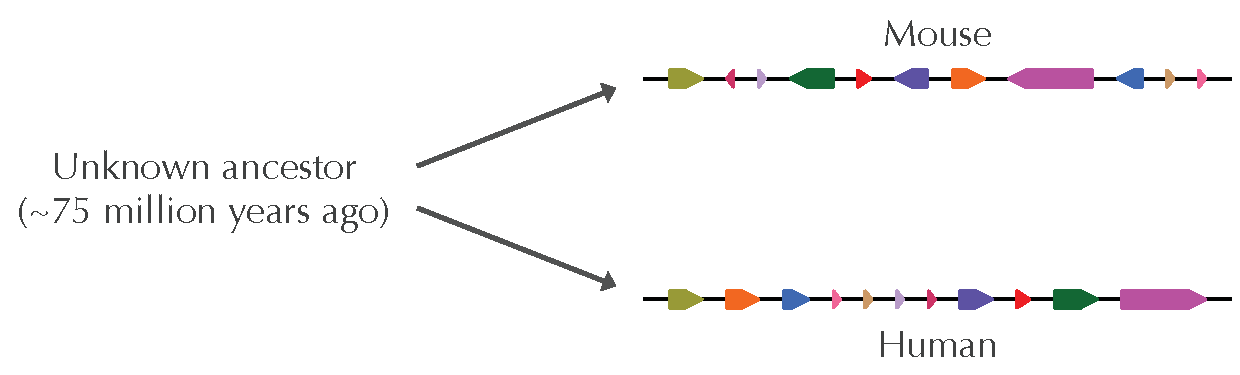
\includegraphics[width=0.88\textwidth]{images/rearrangements/mouse_and_human_synteny_blocks}
\caption{Mouse and human X chromosomes represented as 11 colored, directed segments (synteny blocks).}
\label{fig:mouse_and_human_synteny_blocks}
\end{figure}

\autoref{fig:mouse_and_human_synteny_blocks} offers a compact representation of how the human and mouse X chromosomes differ, but what does it really mean?  It turns out not only that most human genes have mouse counterparts, but also that hundreds of similar genes often line up one after another in the same order in the two species genomes. Each of the 11 colored segments in \autoref{fig:mouse_and_human_synteny_blocks} represents such a procession of similar genes and is called a \textdef{synteny block}. Later, we will explain how to construct synteny blocks and what the left and right \textdef{directions} of the blocks signify.

Synteny blocks simplify the comparison of the mouse and human X chromosomes from 150 million base pairs to only 11 units. This simplification is analogous to comparing two similar photographs. If we compare the images one pixel at a time, we may be overwhelmed by the scale of the problem; instead, we need to zoom out in order to notice higher-level patterns.  It is no accident that biologists use the term ``resolution'' to discuss the level at which genomes are analyzed.

\phantomsection
\subsection{Reversals}
\label{subsec:reversals}

You have probably been wondering how the genome changes when it undergoes a genome rearrangement. Genome rearrangements were discovered 90 years ago when Alfred Sturtevant was studying fruit fly mutants with scarlet- and peach-colored eyes as well as abnormally shaped deltoid wings. Sturtevant determined the genes coding for these traits, called \Red{scarlet}, \Orange{peach}, and \Blue{delta}, and he was amazed to find that the arrangement of these genes in \textit{Drosophila melanogaster} (\Red{scarlet}, \Orange{peach}, \Blue{delta}) differed from their arrangement in \textit{Drosophila simulans} (\Red{scarlet}, \Blue{delta}, \Orange{peach}). He immediately conjectured that the chromosomal segment containing \Orange{peach} and \Blue{delta} must have been flipped around (see \takedetour[Discovery of Genome Rearrangements]{discovery_of_genome_rearrangements}). Sturtevant had witnessed the most common form of genome rearrangement, called a \textdef{reversal}, which flips around an interval of a chromosome and inverts the directions of any synteny blocks within the interval.

\autoref{fig:transforming_mouse_into_human_7_reversals} shows a series of 7 reversals transforming the mouse X chromosome into the human X chromosome.  If this scenario is correct, then the X chromosome of the ancestor of humans and mice must be represented by one of the intermediate synteny block orderings.  Unfortunately, this series of 7 reversals offers only one of 1070 different 7-step scenarios transforming the mouse X chromosome into the human X chromosome. We have no clue which scenario is correct, or even whether the correct scenario had exactly 7 reversals.\\

\begin{qbox}[
Can you convert the mouse X chromosome into the human X chromosome using only 6 reversals?
]\end{qbox}

\begin{figure}[h]
\mySfFamily
\centering
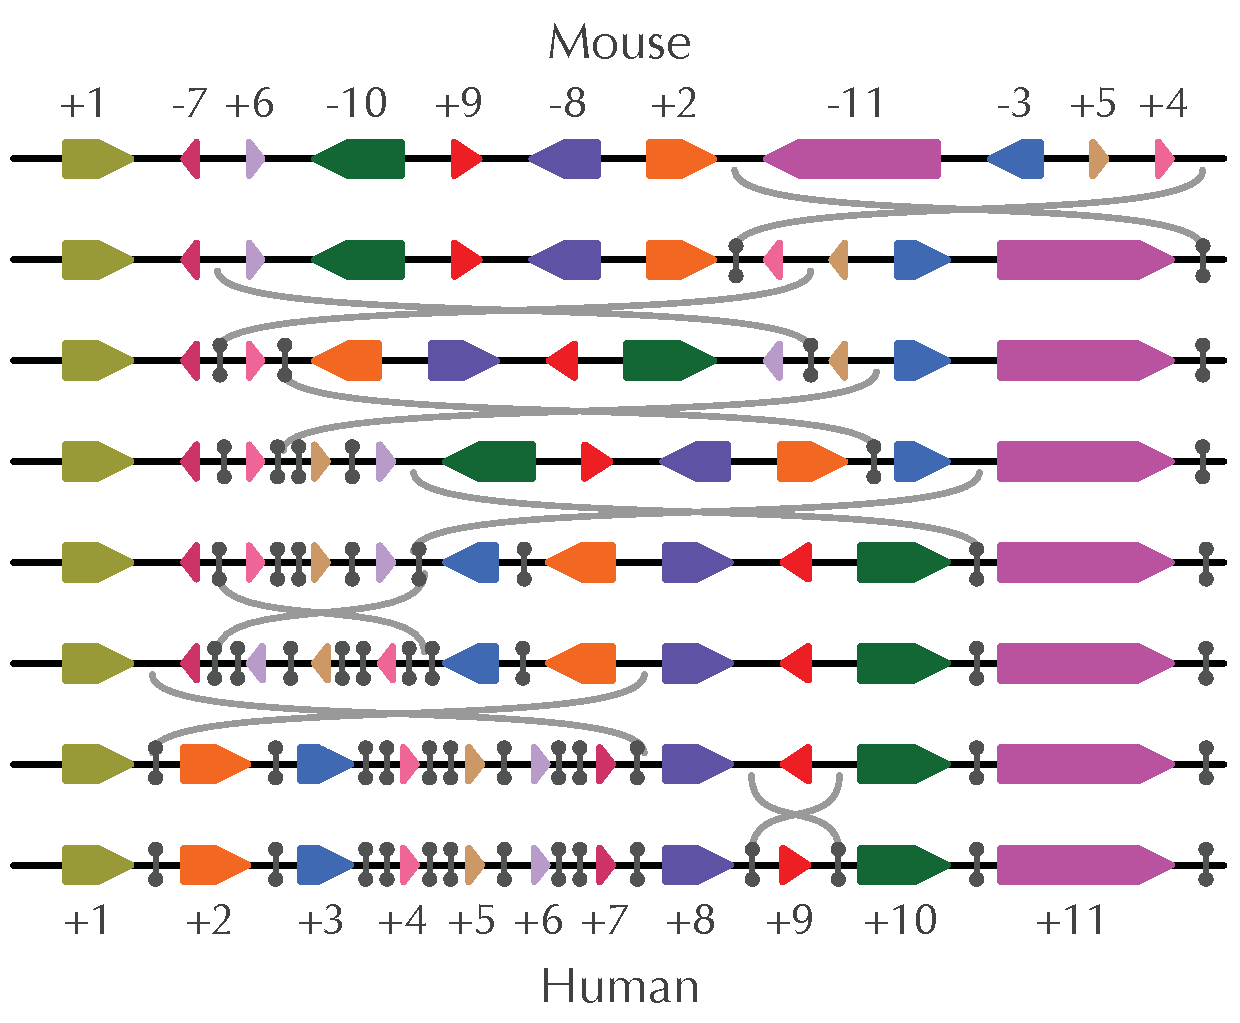
\includegraphics[width=0.8\textwidth]{images/rearrangements/transforming_mouse_into_human_7_reversals}
\caption{Transforming the mouse X chromosome into the human X chromosome with 7 reversals. Each synteny block is uniquely colored and labeled with an integer between 1 and 11; the positive or negative sign of each integer indicates the synteny block's direction (pointing right or left, respectively). Two short vertical segments delineate the endpoints of the inverted interval in each reversal. Suppose that this evolutionary scenario is correct and that, say, the 5th synteny block arrangement from the top presents the true ancestral arrangement. Then the first 4 reversals happened on the evolutionary path from mice to the human-mouse common ancestor (traveling backward in time), and the final 3 reversals happened on the evolutionary path from the common ancestor
to humans (traveling forward in time).  In this chapter, we are not interested in reconstructing the ancestral genome and thus are not concerned with whether a certain reversal travels backward or forward in time.}
\label{fig:transforming_mouse_into_human_7_reversals}
\end{figure}

\noindent Regardless of how many reversals separate the human and mouse X chromosomes, you can see that reversals must be rare genomic events.  Indeed, genome rearrangements typically cause the death or sterility of the mutated organism, thus preventing it from passing the rearrangement on to the next generation.  However, a tiny fraction of genome rearrangements may have a positive effect on survival and propagate through a species as the result of natural selection.  When a population becomes isolated from the rest of its species for long enough, the work of rearrangements can even create a new species.

\phantomsection
\subsection{Rearrangement hotspots}
\label{subsec:rearrangement_hotspots}

Geology provides a thought-provoking analogy for thinking about genome evolution.  You might like to think of genome rearrangements as ``genomic earthquakes'' that dramatically change the chromosomal architecture of an organism.  Genome rearrangements contrast with much more frequent point mutations, which work slowly and are analogous to ``genomic erosion''.

You can visualize a reversal as breaking the genome on both sides of a chromosomal interval, flipping the interval, and then gluing the resulting segments in a new order. Keeping in mind that earthquakes occur more frequently in specific locations on Earth, we wonder if a similar principle holds for reversals --- are they happening over and over again in specific genomic regions?  A fundamental question in chromosome evolution studies is whether the \textdef{breakpoints} of reversals (i.e., the the ends of the inverted intervals) occur along ``fault lines'' called \textdef{rearrangement hotspots}. If such hotspots exist in the human genome, we want to locate them and determine how they might relate to genetic disorders, which are often attributable to rearrangements.

Of course, we should rigorously define what we mean by a ``rearrangement hotspot''. Re-examining the 7-reversal scenario changing the mouse X chromosome into the human X chromosome in \autoref{fig:transforming_mouse_into_human_7_reversals}, we record the endpoints of each reversal using vertical segments. Regions affected by multiple reversals are indicated by multiple vertical segments in the human X chromosome. For example, the region adjacent to the pointed side of block 3 in \autoref{fig:transforming_mouse_into_human_7_reversals} is used as an endpoint of both the 4th and 5th reversals. As a result, we have placed two vertical lines between blocks 3 and 4 in the human X chromosome. However, just because we showed two breakpoints in this region does not imply that this region is a rearrangement hotspot, since the reversals in \autoref{fig:transforming_mouse_into_human_7_reversals} represent just one possible evolutionary scenario. Because the true rearrangement scenario is unknown, it is not immediately clear how we could determine whether rearrangement hotspots exist.\\

\phantomsection
\FloatBarrier
\section{The Random Breakage Model of Chromosome Evolution}
\label{sec:the_random_breakage_model_of_chromosome_evolution}

In 1973, Susumu Ohno proposed the \textdef{Random Breakage Model} of chromosome evolution.  This hypothesis states that the breakpoints of rearrangements are selected randomly, implying that rearrangement hotspots in mammalian genomes do not exist.  Yet this model lacked supporting evidence when it was introduced.  After all, how could we possibly determine whether rearrangement hotspots exist without knowing the exact sequence of rearrangements separating two species?\\

\begin{qbox}[
Consider the following questions.
\vspace{-1ex}
\begin{enumerate}
\item Say that a series of random reversals result in one huge synteny block covering 90\% of the genome in addition to 99 tiny synteny blocks covering the remaining 10\% of the genome.  Should we be surprised?
\vspace{-1ex}
\item What if random reversals result in 100 synteny blocks of roughly the same length? Should we be surprised?
\end{enumerate}
\vspace{-1ex}
]\end{qbox}

\noindent The idea that we wish to impress on you in the preceding questions is that we can test the Random Breakage Model by analyzing the distribution of synteny block lengths. For example, the lengths of the human-mouse synteny blocks on the X chromosome vary widely, with the largest block (block 11 in \autoref{fig:transforming_mouse_into_human_7_reversals}) taking up nearly 25\% of the entire length of the X chromosome. Is this variation in synteny block length consistent with the Random Breakage Model?\\

\begin{figure}[h]
\centering
\begin{tabular}{c}
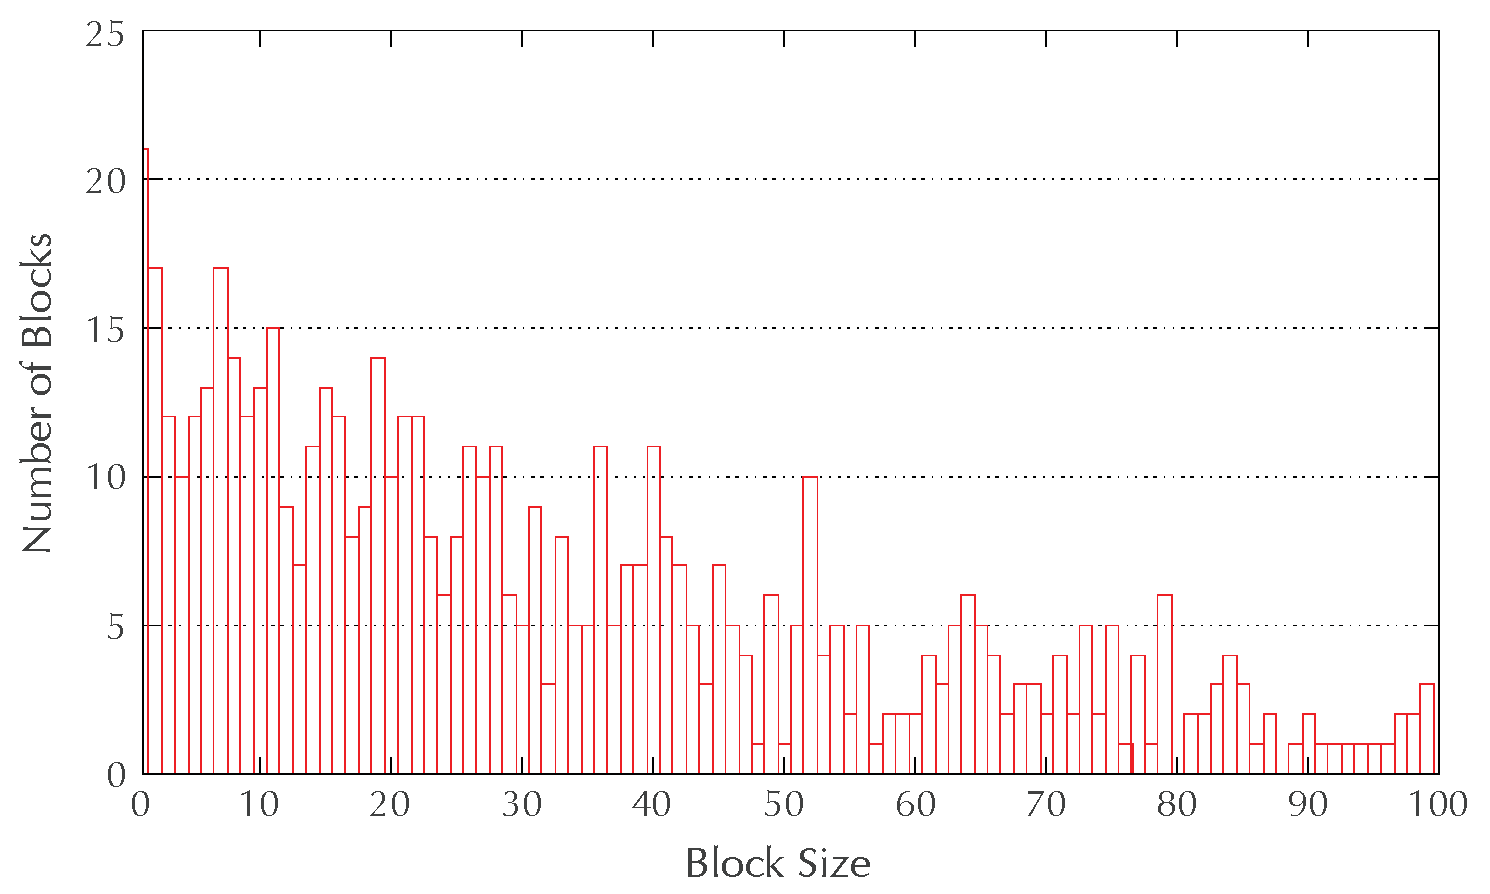
\includegraphics[width = 0.65\textwidth]{images/rearrangements/histogram_exponential_distribution_one_run}\\[2ex]
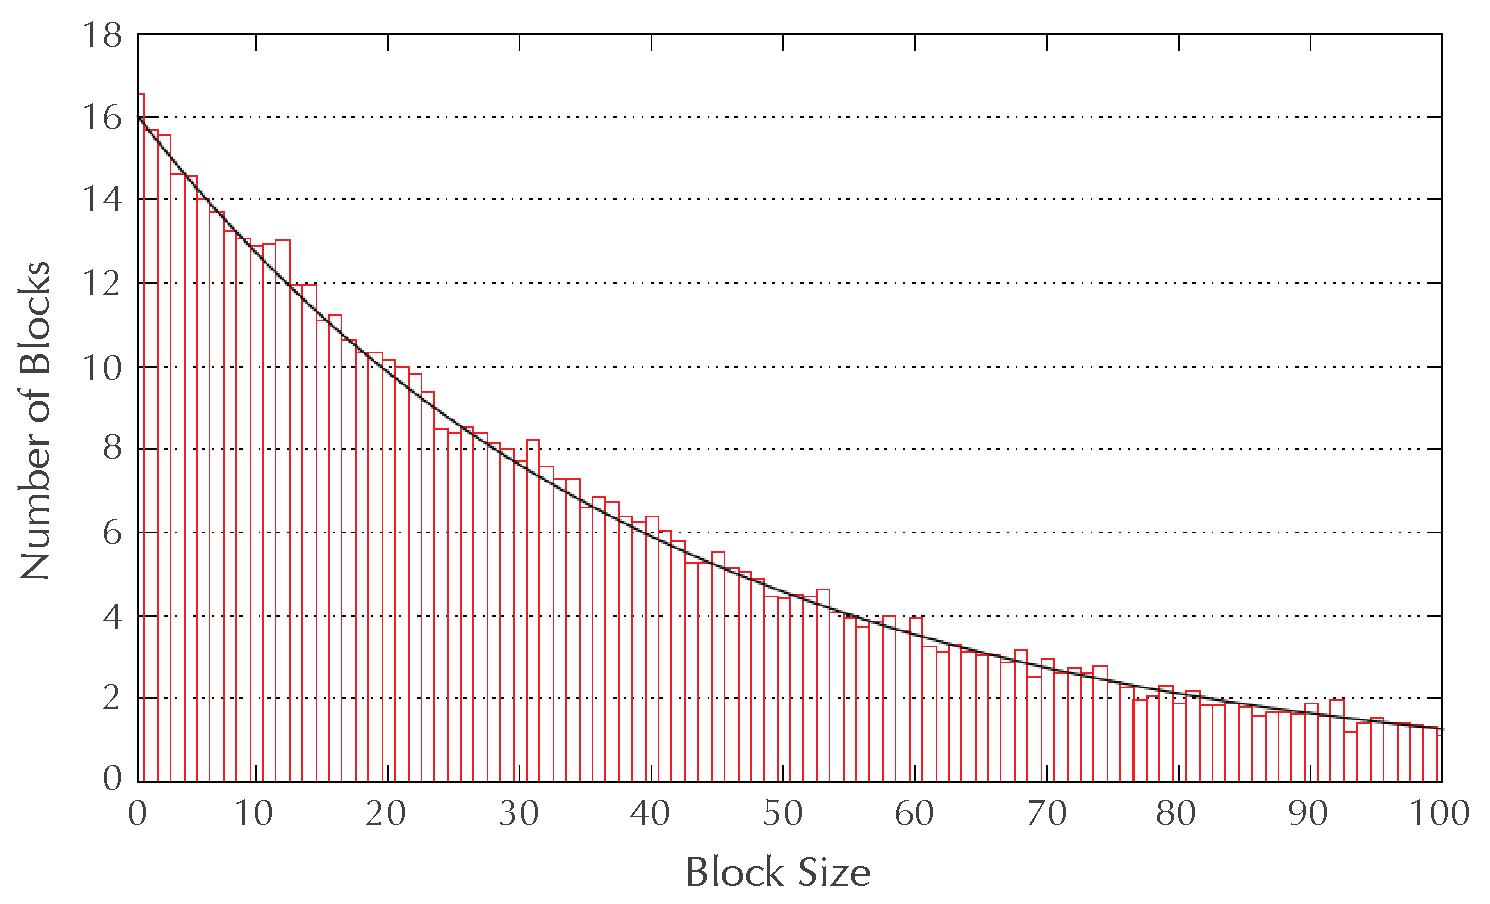
\includegraphics[width = 0.65\textwidth]{images/rearrangements/histogram_exponential_distribution_many_runs}
\end{tabular}
\caption{(Top) A histogram showing the number of blocks of each size (for a simulated genome with 25,000 genes after 320 randomly chosen reversals). Blocks having more than 100 genes are not shown. (Bottom) An average histogram of synteny block lengths for 100 simulations, fitted by the exponential distribution.}
\label{fig:histogram_exponential_distribution}
\end{figure}

In 1984, Joseph Nadeau and Benjamin Taylor asked what the expected lengths of synteny blocks should be after $N$ reversals occurring at random locations in the genome.  If we rule out the unlikely event that two random reversals cut the chromosome in exactly the same position, then $N$ random reversals cut the chromosome in $2N$ locations and produce $2N + 1$ synteny blocks. \autoref{fig:histogram_exponential_distribution} (top) depicts the result of a computational experiment in which 320 random reversals are applied to a simulated chromosome consisting of 25,000 genes, producing $2 \cdot 320+1 = 641$ synteny blocks. The average synteny block size is 25,000$/641 \approx 34$ genes, but this does not mean that all synteny blocks should have approximately 34 genes. If we select random locations for breakpoints, then some blocks may have only a few genes, whereas other blocks may contain over a hundred.  The point is that regardless of how many times we run this simulation, the resulting distributions of synteny block lengths will be similar. \autoref{fig:histogram_exponential_distribution} (bottom) averages the results of 100 such simulations and illustrates that the distribution of synteny block lengths can be approximated by a curve corresponding to an \textdef{exponential distribution} (see \takedetour[The Exponential Distribution]{the_exponential_distribution}).  The exponential distribution predicts that we should observe about seven blocks having 34 genes and one or two much larger blocks having 100 genes.

What happens when we look at the histogram for the real human and mouse synteny blocks? When Nadeau and Taylor constructed this histogram for the limited genetic data available in 1984, they observed that the lengths of blocks fit the exponential distribution well.  In the 1990s, more accurate synteny block data fit the exponential distribution even better (\autoref{fig:histogram_human_mouse_synteny_blocks}). Case closed --- even though we don't know the exact rearrangements causing our genome to evolve over the last 75 million years, these rearrangements must have followed the Random Breakage Model!\\

\begin{figure}[h]
\mySfFamily
\centering
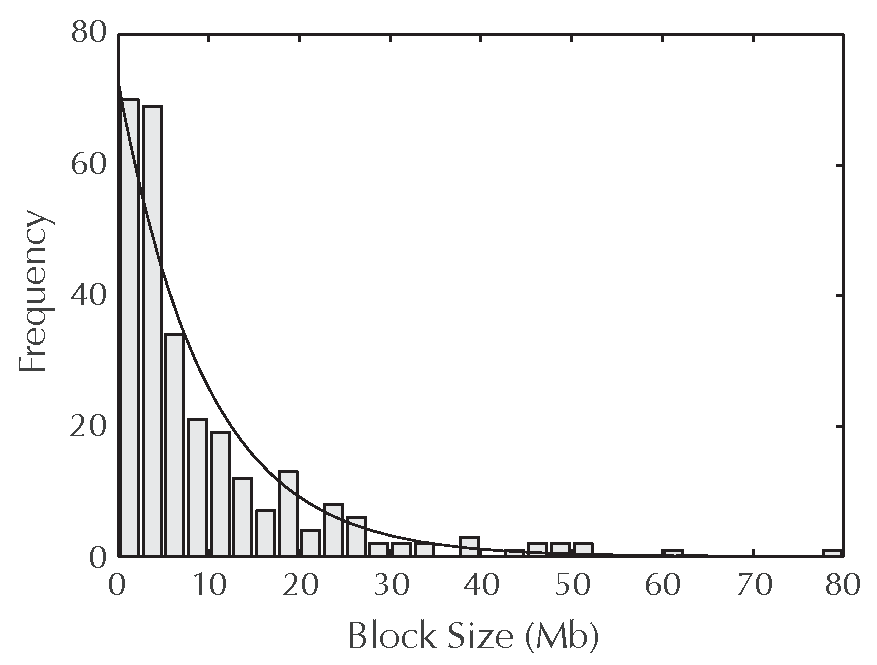
\includegraphics[width=0.45\textwidth]{images/rearrangements/histogram_human_mouse_synteny_blocks}
\caption{Histogram of human-mouse synteny block lengths (only synteny blocks longer than 1 million nucleotides are shown). The histogram is fitted by an exponential distribution.}
\label{fig:histogram_human_mouse_synteny_blocks}
\end{figure}

\begin{qbox}[
Do you agree with the logic behind this argument?
]\end{qbox}

\vspace{-2\baselineskip}

\phantomsection
\FloatBarrier
\section{Sorting by Reversals}
\label{sec:sorting_by_reversals}

We now have evidence in favor of the Random Breakage Model, but this evidence is far from conclusive.  To test this model, let's start building a mathematical model for rearrangement analysis.  We will therefore return to a problem that we hinted at the introduction, which is finding the minimum number of reversals that could transform the mouse X chromosome into the human X chromosome.\\

\begin{qbox}[
From a biological perspective, why do you think we want to find the minimum possible number of reversals?
]\end{qbox}

\noindent We ask for the minimum number of reversals in accordance with the principle of \textdef{Occam's razor}. This maxim states that when presented with some quandary, we should explain it using the simplest hypothesis that is consistent with what we already know. In this case, it seems most reasonable that evolution would take the ``shortest path'' connecting two species, i.e., the most \textdef{parsimonious} evolutionary scenario. Evolution may not always take the shortest path, but even when it does not, the number of steps in the true evolutionary scenario often comes close to the number of steps in the most parsimonious scenario.  How, then, can we find the length of this shortest path?

Genome rearrangement studies typically ignore the lengths of synteny blocks and represent chromosomes by \textdef{signed permutations}. Each block is labeled by a number, which is assigned a positive/negative sign depending on the block's direction.  The number of elements in a signed permutation is its \textdef{length}. As you can see from \autoref{fig:transforming_mouse_into_human_7_reversals}, the human and mouse X chromosomes can be represented by the following signed permutations of length 11:

\begin{center}
\tabcolsep = 0.3em
\begin{tabular}{rr @{\hskip 0em} rrrrrrrrrrrl}
\textbf{Mouse:} & ( & $+1$ & $-7$ & $+6$ & $-10$ & $+9$ & $-8$ & $+2$ & $-11$ & $-3$ & $+5$ & $+4)$\\
\textbf{Human:} & ( & $+1$ & $+2$ & $+3$ & $+4$ & $+5$ & $+6$ & $+7$ & $+8$ & $+9$ & $+10$ & $+11)$
\end{tabular}
\end{center}

\noindent In the rest of the chapter, we will refer to signed permutations as \textdef{permutations} for short. Because we assume that each synteny block is unique, we do not allow repeated numbers in permutations (e.g., $(+1$ $-2$ $+3$ $+2)$ is not a permutation).\\

\begin{exercise}[
How many permutations of length $n$ are there?
]\end{exercise}

\vspace{-0.5\baselineskip}

\noindent We can model reversals by inverting the elements within an interval of a permutation, then switching the signs of any elements within the inverted interval. For example, the cartoon in \autoref{fig:reversal_cartoon} illustrates how a reversal changes the permutation $(+1$ $+2$ $+3$ $\MathRed{+4}$ $\MathRed{+5}$ $\MathRed{+6}$ $\MathRed{+7}$ $\MathRed{+8}$ $+9$ $+10)$ into $(+1$ $+2$ $+3$ $\MathRed{-8}$ $\MathRed{-7}$ $\MathRed{-6}$ $\MathRed{-5}$ $\MathRed{-4}$ $+9$ $+10)$.  This reversal can be viewed as first breaking the permutation between +3 and +4 as well as between +8 and +9:

\begin{center}
$(+1$ $+2$ $+3)$$(\MathRed{+4}$ $\MathRed{+5}$ $\MathRed{+6}$ $\MathRed{+7}$ $\MathRed{+8})$$(+9$ $+10)$
\end{center}

\begin{figure}[t]
\centering
\begin{tabular}{c @{\hskip 2.5em} c}
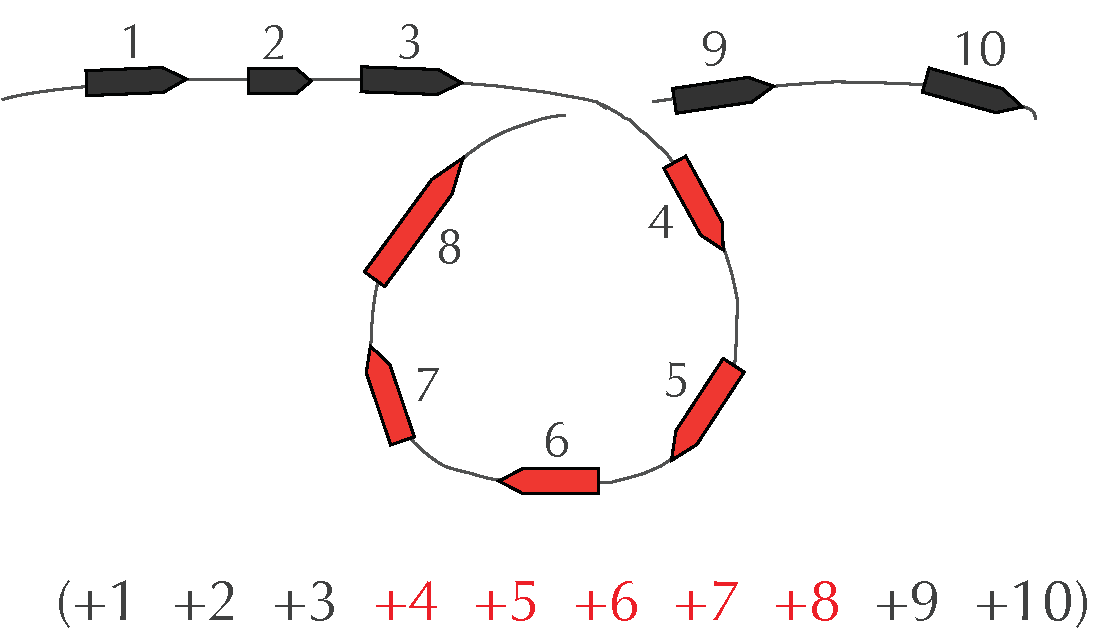
\includegraphics[width = 0.4\textwidth]{images/rearrangements/reversal_cartoon-1} & 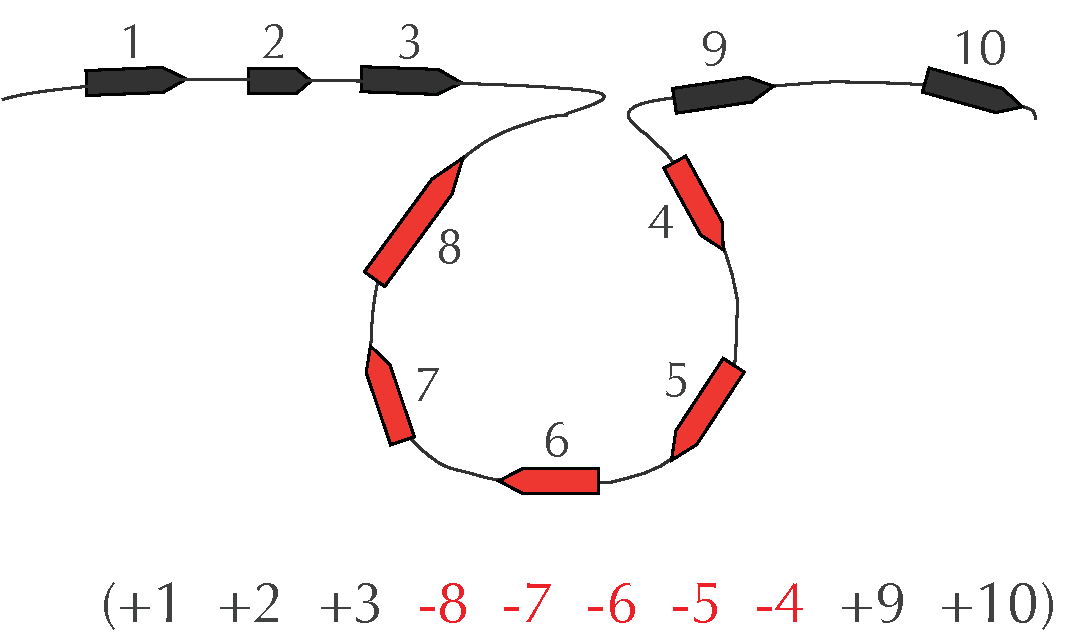
\includegraphics[width = 0.4\textwidth]{images/rearrangements/reversal_cartoon-2}
\end{tabular}
\caption{A cartoon illustrating how a reversal breaks a chromosome in two places and inverts the segment between the two breakpoints. Note that the reversal changes the sign of each element within the permutation's inverted segment.}
\label{fig:reversal_cartoon}
\end{figure}

\noindent It then inverts this middle segment:

\begin{center}
$(+1$ $+2$ $+3)$$(\MathRed{-8}$ $\MathRed{-7}$ $\MathRed{-6}$ $\MathRed{-5}$ $\MathRed{-4})$$(+9$ $+10)$
\end{center}

\noindent and finally glues the three segments back together to form a new permutation:

\begin{center}
$(+1$ $+2$ $+3$ $\MathRed{-8}$ $\MathRed{-7}$ $\MathRed{-6}$ $\MathRed{-5}$ $\MathRed{-4}$ $+9$ $+10)$
\end{center}

\fudgespace

\begin{exercise}[
How many different reversals can be applied to a permutation of length $n$?
]\end{exercise}

\noindent We define the \textdef{reversal distance} between permutations $P$ and $Q$, denoted $d_{\text{rev}}(P, Q)$, as the minimum number of reversals required to transform $P$ into $Q$.\\

\begin{problem}[Reversal Distance Problem]{Calculate the reversal distance between two permutations.}{Two permutations of equal length.}{The reversal distance between these permutations.}
\end{problem}

\vspace{-\baselineskip}

\noindent We represented the human X chromosome by $(+1$ $+2$ $+3$ $+4$ $+5$ $+6$ $+7$ $+8$ $+9$ $+10$ $+11)$; this permutation, in which blocks are ordered from smallest to largest with positive directions, is called the \textdef{identity permutation}. The reason why we used the identity permutation of length 11 to represent the human X chromosome is that when comparing two genomes, we can label the synteny blocks in one of the genomes however we like. The block labeling for which the human X chromosome is the identity permutation automatically induces the representation of the mouse chromosome as $(+1$ $-7$ $+6$ $-10$ $+9$ $-8$ $+2$ $-11$ $-3$ $+5$ $+4)$.   Of course, we could have instead encoded the mouse X chromosome as the identity permutation, which would have induced the encoding of the human X chromosome as $(+1$ $+7$ $-9$ $+11$ $+10$ $+3$ $-2$ $-6$ $+5$ $-4$ $-8)$ (\autoref{fig:x_chromosomes_different_encoding}).\\

\begin{figure}[h]
\centering
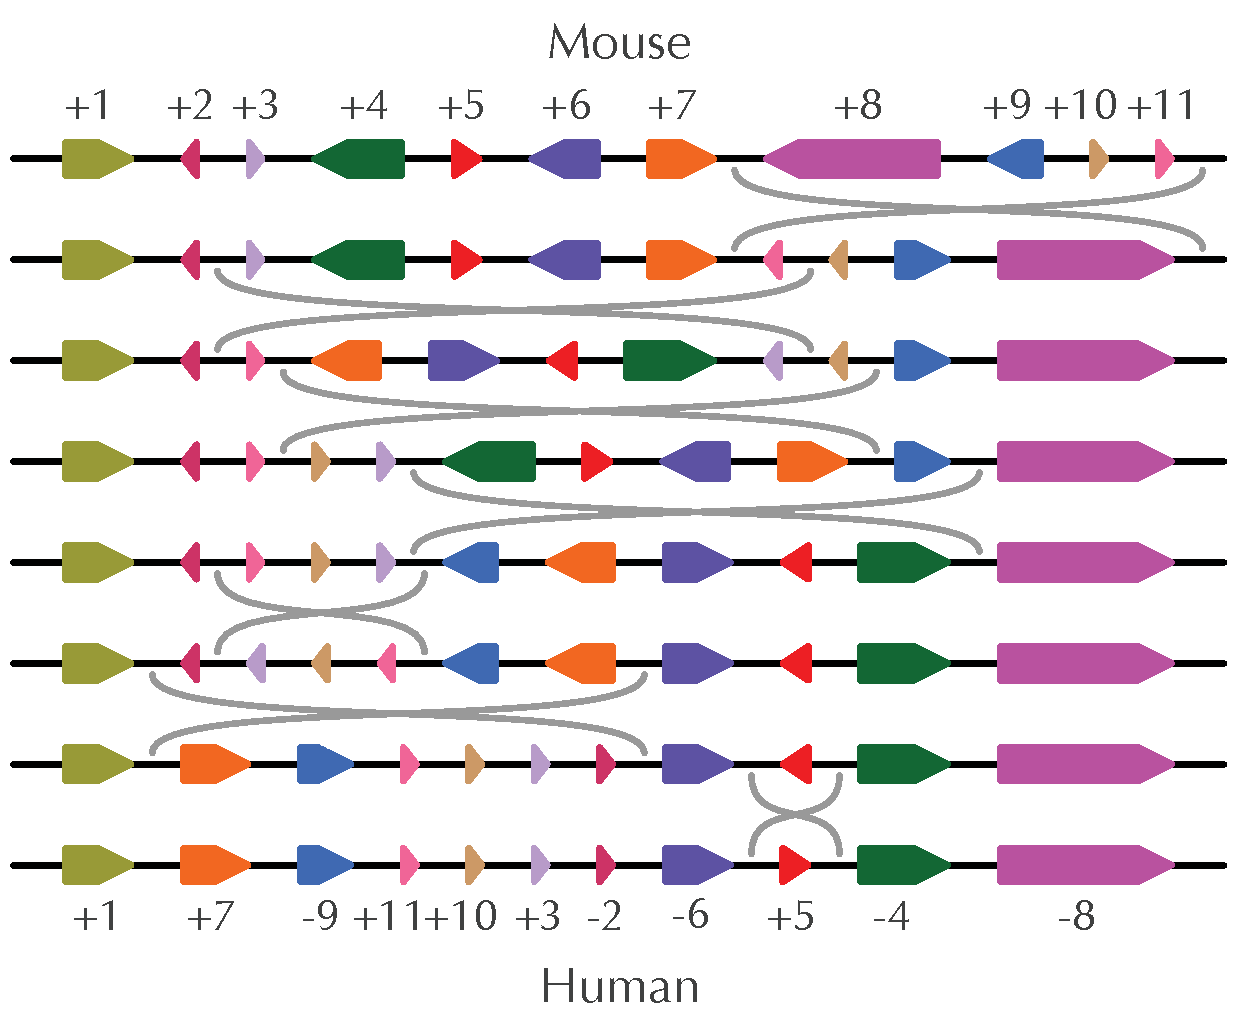
\includegraphics[width = 0.8\textwidth]{images/rearrangements/x_chromosomes_different_encoding}
\caption{Encoding the mouse X chromosome as the identity permutation implies encoding the human X chromosome as $(+1$ $+7$ $-9$ $+11$ $+10$ $+3$ $-2$ $-6$ $+5$ $-4$ $-8)$.}
\label{fig:x_chromosomes_different_encoding}
\end{figure}

\begin{qbox}[
Is the reversal distance between $(+1$ $+2$ $+3$ $+4$ $+5$ $+6$ $+7$ $+8$ $+9$ $+10$ $+11)$ and $(+1$ $-7$ $+6$ $-10$ $+9$ $-8$ $+2$ $-11$ $-3$ $+5$ $+4)$ equal to the reversal distance between $(+1$ $+2$ $+3$ $+4$ $+5$ $+6$ $+7$ $+8$ $+9$ $+10$ $+11)$ and $(+1$ $+7$ $-9$ $+11$ $+10$ $+3$ $-2$ $-6$ $+5$ $-4$ $-8)$?  In other words, does the specific labeling of synteny blocks affect the reversal distance between the two chromosomes?
]\end{qbox}

\noindent Because we have the freedom to label synteny blocks however we like, we will consider an offshoot of the Reversal Distance Problem in which permutation $Q$ is the identity permutation  $(+1$ $+2$ \ldots $+n)$. This computational problem is called \textdef{sorting by reversals}, and we denote the minimum number of reversals required to sort $P$ into the identity permutation as $d_{\text{rev}}(P)$.  The history of sorting by reversals is founded in a culinary application and involves two celebrities (see \takedetour[Bill Gates and David X. Cohen Flip Pancakes]{bill_gates_and_david_x_cohen_flip_pancakes}).\\

\begin{problem}[Sorting by Reversals Problem]{Compute the reversal distance between a permutation and the identity permutation.}{A permutation $P$.}{The reversal distance $d_{\text{rev}}(P)$.}
\end{problem}

\noindent Here is a sorting of $(+2$ $-4$ $-3$ $+5$ $-8$ $-7$ $-6$ $+1)$ using five reversals, with the inverted interval at each step shown in red:

\begin{center}
\begin{math}
\arraycolsep = 0.3em
\begin{array}{r @{\hskip 0em} r r r r r r r r @{\hskip 0em} l}
( & +2 & \MathRed{-4} & \MathRed{-3} & +5 & -8 & -7 & -6 & +1 &)\\[-0.25ex]
( & +2 & +3 & +4 & +5 & \MathRed{-8} & \MathRed{-7} & \MathRed{-6} & +1 &)\\[-0.25ex]
( & +2 & +3 & +4 & +5 & +6 & +7 & +8 & \MathRed{+1} &)\\[-0.25ex]
( & \MathRed{+2} & \MathRed{+3} & \MathRed{+4} & \MathRed{+5} & \MathRed{+6} & \MathRed{+7} & \MathRed{+8} & -1 &)\\[-0.25ex]
( & \MathRed{-8} & \MathRed{-7} & \MathRed{-6} & \MathRed{-5} & \MathRed{-4} & \MathRed{-3} & \MathRed{-2} & \MathRed{-1} &)\\[-0.25ex]
( & +1 & +2 & +3 & +4 & +5 & +6 & +7 & +8 &)
\end{array}
\end{math}
\end{center}

\begin{qbox}[
Can you sort this permutation using fewer reversals?
]\end{qbox}

\vspace{-0.5\baselineskip}

\noindent Here is a faster sorting:

\begin{center}
\begin{math}
\arraycolsep = 0.3em
\begin{array}{r @{\hskip 0em} r r r r r r r r @{\hskip 0em} l}
( & +2 & \MathRed{-4} & \MathRed{-3} & +5 & -8 & -7 & -6 & +1 &)\\[-0.25ex]
( & \MathRed{+2} & \MathRed{+3} & \MathRed{+4} & \MathRed{+5} & -8 & -7 & -6 & +1 &)\\[-0.25ex]
( & -5 & -4 & -3 & -2 & \MathRed{-8} & \MathRed{-7} & \MathRed{-6} & \MathRed{+1} &)\\[-0.25ex]
( & \MathRed{-5} & \MathRed{-4} & \MathRed{-3} & \MathRed{-2} & \MathRed{-1} & +6 & +7 & +8 &)\\[-0.25ex]
( & +1 & +2 & +3 & +4 & +5 & +6 & +7 & +8 &)
\end{array}
\end{math}
\end{center}

\begin{qbox}[
Consider the following questions.
\vspace{-1ex}
\begin{enumerate}
\item Is it possible to sort this permutation even faster?
\vspace{-1ex}
\item During sorting by reversals, the intermediate permutations in the example above are getting more and more ``ordered''. Can you come up with a quantitative measure of how ordered a permutation is?
\vspace{-1ex}
\end{enumerate}
]\end{qbox}

%\vspace{-2\baselineskip}

\phantomsection
\FloatBarrier
\section{A Greedy Algorithm for Sorting by Reversals}
\label{sec:a_greedy_algorithm_for_sorting_by_reversals}

Let's see if we can design a greedy heuristic to approximate $d_{\text{rev}}(P)$. The simplest idea is to first fix $+1$ in the first position, then fix $+2$ in the second position, and so on.  For example, element 1 is already in the correct position and has the correct sign in the mouse X chromosome, but element 2 is not in the correct position. We can keep element 1 fixed and move element 2 to the correct position by applying a single reversal.

\begin{center}
\begin{math}
\arraycolsep = 0.3em
\begin{array}{r @{\hskip 0em} r r r r r r r r r r r @{\hskip 0em} l}
( & \MathBlue{+1} & \MathRed{-7} & \MathRed{+6} & \MathRed{-10} & \MathRed{+9} & \MathRed{-8} & \MathRed{+2} & -11 & -3 & +5 & +4 &)\\[-0.25ex]
( & \MathBlue{+1} & -2 & +8 & -9 & +10 & -6 & +7 & -11 & -3 & +5 & +4 &)\\
\end{array}
\end{math}
\end{center}

\noindent One more reversal flips element 2 around so that it has the correct sign:

\begin{center}
\begin{math}
\centering
\arraycolsep = 0.3em
\begin{array}{r @{\hskip 0em} r r r r r r r r r r r  @{\hskip 0em} l}
( & \MathBlue{+1} & \MathRed{-2} & +8 & -9 & +10 & -6 & +7 & -11 & -3 & +5 & +4 &)\\[-0.25ex]
( & \MathBlue{+1} & \MathBlue{+2} & +8 & -9 & +10 & -6 & +7 & -11 & -3 & +5 & +4 &)
\end{array}
\end{math}
\end{center}

\noindent By iterating, we can successively move larger and larger elements to their correct positions in the identity permutation by following the reversals below.  The inverted interval of each reversal is still shown in red, and elements that have been placed in the correct position are shown in blue.

\begin{center}
\begin{math}
\arraycolsep = 0.2em
\begin{array}{r @{\hskip 0em} r r r r r r r r r r r @{\hskip 0em} l}
( & \MathBlue{+1} & \MathRed{-7} & \MathRed{+6} & \MathRed{-10} & \MathRed{+9} & \MathRed{-8} & \MathRed{+2} & -11 & -3 & +5 & +4 &)\\[-0.25ex]
( & \MathBlue{+1} & \MathRed{-2} & +8 & -9 & +10 & -6 & +7 & -11 & -3 & +5 & +4 &)\\[-0.25ex]
( & \MathBlue{+1} & \MathBlue{+2} & \MathRed{+8} & \MathRed{-9} & \MathRed{+10} & \MathRed{-6} & \MathRed{+7} & \MathRed{-11} & \MathRed{-3} & +5 & +4 &)\\[-0.25ex]
( & \MathBlue{+1} & \MathBlue{+2} & \MathBlue{+3} & \MathRed{+11} & \MathRed{-7} & \MathRed{+6} & \MathRed{-10} & \MathRed{+9} & \MathRed{-8} & \MathRed{+5} & \MathRed{+4} &)\\[-0.25ex]
( & \MathBlue{+1} & \MathBlue{+2} & \MathBlue{+3} & \MathRed{-4} & -5 & +8 & -9 & +10 & -6 & +7 & -11 &)\\[-0.25ex]
( & \MathBlue{+1} & \MathBlue{+2} & \MathBlue{+3} & \MathBlue{+4} & \MathRed{-5} & +8 & -9 & +10 & -6 & +7 & -11 &)\\[-0.25ex]
( & \MathBlue{+1} & \MathBlue{+2} & \MathBlue{+3} & \MathBlue{+4} & \MathBlue{+5} & \MathRed{+8} & \MathRed{-9} & \MathRed{+10} & \MathRed{-6} & +7 & -11 &)\\[-0.25ex]
( & \MathBlue{+1} & \MathBlue{+2} & \MathBlue{+3} & \MathBlue{+4} & \MathBlue{+5} & \MathBlue{+6} & \MathRed{-10} & \MathRed{+9} & \MathRed{-8} & \MathRed{+7} & -11 &)\\[-0.25ex]
( & \MathBlue{+1} & \MathBlue{+2} & \MathBlue{+3} & \MathBlue{+4} & \MathBlue{+5} & \MathBlue{+6} & \MathRed{-7} & +8 & -9 & +10 & -11 &)\\[-0.25ex]
( & \MathBlue{+1} & \MathBlue{+2} & \MathBlue{+3} & \MathBlue{+4} & \MathBlue{+5} & \MathBlue{+6} & \MathBlue{+7} & \MathBlue{+8} & \MathRed{-9} & +10 & -11 &)\\[-0.25ex]
( & \MathBlue{+1} & \MathBlue{+2} & \MathBlue{+3} & \MathBlue{+4} & \MathBlue{+5} & \MathBlue{+6} & \MathBlue{+7} & \MathBlue{+8} & \MathBlue{+9} & \MathBlue{+10} & \MathRed{-11} &)\\[-0.25ex]
( & \MathBlue{+1} & \MathBlue{+2} & \MathBlue{+3} & \MathBlue{+4} & \MathBlue{+5} & \MathBlue{+6} & \MathBlue{+7} & \MathBlue{+8} & \MathBlue{+9} & \MathBlue{+10} & \MathBlue{+11} &)\\[-0.25ex]
\end{array}
\end{math}
\end{center}

This example motivates a greedy heuristic called \textalg{GreedySorting}.  We say that element $k$ in permutation $P = (p_1 \ldots p_n)$ is \textdef{sorted} if $p_k = +k$ and \textdef{unsorted} otherwise.  For every unsorted element $k$ that is located outside the first $k$ positions in $P$, there exists a single reversal, called the \textdef{\textit{k}-sorting reversal}, which fixes the first $k - 1$ elements of $P$ and moves element $k$ to the $k$-th position.  For example, in the sorting of the mouse X chromosome shown above, the 2-sorting reversal transforms $(\MathBlue{+1}$ $\MathRed{-7}$ $\MathRed{+6}$ $\MathRed{-10}$ $\MathRed{+9}$ $\MathRed{-8}$ $\MathRed{+2}$ $-11$ $-3$ $+5$ $+4)$ into $(\MathBlue{+1}$ $-2$ $+8$ $-9$ $+10$ $-6$ $+7$ $-11$ $-3$ $+5$ $+4)$.  In this case, one additional reversal flipping $-2$ around was needed to sort element 2.

We now give the pseudocode for \textalg{GreedySorting}, which applies $k$-sorting reversals for increasing values of $k$.  Here, $|P|$ refers to the length of permutation $P$.\\

\begin{elaboration}
\begin{algorithmic}
\leftskip = \algindent %Needed to match the indentation of the text.
\Algorithm{GreedySorting}{\textvar{P}}
	\State $\textvar{approxReversalDistance} \gets 0$
	\For {$k \gets 1$ to $|P|$}
		\If {element $k$ is not sorted}
			\State apply the $k$-sorting reversal to $P$
			\State $\textvar{approxReversalDistance} \gets \textvar{approxReversalDistance} + 1$
			\If {$k$-th element of $P$ is $-k$}
				\State apply the reversal flipping the $k$-th element of $P$
				\State $\textvar{approxReversalDistance} \gets \textvar{approxReversalDistance} + 1$
			\EndIf
		\EndIf
	\EndFor
	\State \return{~\textvar{approxReversalDistance}}
\EndAlgorithm
\end{algorithmic}
\end{elaboration}
\protect\computationalproblem[Implement \textalg{GreedySorting}]{-21.68}

\noindent In the case of the mouse X chromosome, \textalg{GreedySorting} requires 11 reversals, but we already know that this permutation can be sorted with 7 reversals, which causes us to wonder: how good of a heuristic is \textalg{GreedySorting}?\\

\begin{exercise}[
What is the largest number of reversals \textalg{GreedySorting} could ever require to sort a permutation of length $n$?
]\end{exercise}

\noindent Consider the permutation $(-6$ $+1$ $+2$ $+3$ $+4$ $+5)$.  You can verify that the greedy heuristic requires ten steps to sort this permutation, and yet it can be sorted using just two reversals!

\begin{center}
\begin{math}
\arraycolsep = 0.3em
\begin{array}{r @{\hskip 0em} r r r r r r @{\hskip 0em} l}
( & \MathRed{-6} & \MathRed{+1} & \MathRed{+2} & \MathRed{+3} & \MathRed{+4} & \MathRed{+5} &)\\[-0.25ex]
( & \MathRed{-5} & \MathRed{-4} & \MathRed{-3} & \MathRed{-2} & \MathRed{-1} & +6 &)\\[-0.25ex]
( & +1 & +2 & +3 & +4 & +5 & +6 &)
\end{array}
\end{math}
\end{center}

\noindent This example demonstrates that \textalg{GreedySorting} provides a poor approximation for the reversal distance.\\

\begin{qbox}[
Can you find a \textit{lower} bound on $d_{\text{rev}}(P)$?  For example, can you show that the mouse permutation $(+1$ $-7$ $+6$ $-10$ $+9$ $-8$ $+2$ $-11$ $-3$ $+5$ $+4)$ cannot be sorted with fewer than 7 reversals?
]\end{qbox}

\phantomsection
\FloatBarrier
\section{Breakpoints}
\label{sec:breakpoints}

\phantomsection
\subsection{What are breakpoints?}
\label{subsec:what_are_breakpoints}

%\begin{center}
%\begin{math}
%\arraycolsep = 0.3em
%\begin{array}{r @{\hskip 0em} r r r r r r r r r r r r r r @{\hskip 0em} l}
%( & +3 & +4 & +5 & \MathRed{-12} & \MathRed{-8} & \MathRed{-7} & \MathRed{-6} & \MathRed{+1} & \MathRed{+2} & \MathRed{+10} & \MathRed{+9} & \MathRed{-11} & +13 & +14 &)\\
%( & \MathRed{+3} & \MathRed{+4} & \MathRed{+5} & \MathRed{+11} & \MathRed{-9} & \MathRed{-10} & \MathRed{-2} & \MathRed{-1} & +6 & +7 & +8 & +12 & +13 & +14 &)\\
%( & +1 & +2 & \MathRed{+10} & \MathRed{+9} & \MathRed{-11} & \MathRed{-5} & \MathRed{-4} & \MathRed{-3} & +6 & +7 & +8 & +12 & +13 & +14 &)\\
%( & +1 & +2 & +3 & +4 & +5 & \MathRed{+11} & \MathRed{-9} & -10 & +6 & +7 & +8 & +12 & +13 & +14 &)\\
%( & +1 & +2 & +3 & +4 & +5 & +9 & \MathRed{-11} & \MathRed{-10} & \MathRed{+6} & \MathRed{+7} & \MathRed{+8} & +12 & +13 & +14 &)\\
%( & +1 & +2 & +3 & +4 & +5 & \MathRed{+9} & \MathRed{-8} & \MathRed{-7} & \MathRed{-6} & +10 & +11 & +12 & +13 & +14 &)\\
%( & +1 & +2 & +3 & +4 & +5 & +6 & +7 & +8 & \MathRed{-9} & +10 & +11 & +12 & +13 & +14 &)\\
%( & +1 & +2 & +3 & +4 & +5 & +6 & +7 & +8 & +9 & +10 & +11 & +12 & +13 & +14 &)\\
%\end{array}
%\end{math}
%\end{center}

Consider the sorting by reversals shown in \autoref{fig:sorting_by_reversals}. We would like to quantify how each subsequent permutation is moving closer to the identity as we apply subsequent reversals. Consider the first reversal; at the right endpoint of the inverted interval, it changes the consecutive elements $(-11$ $+13)$ into the much more desirable $(+12$ $+13)$.  Less obvious is the work of the fourth reversal, which places $-11$ immediately left of $-10$ so that in the next step, the consecutive elements $(-11$ $-10)$ can be part of an inverted interval, creating the desirable consecutive elements  $(+10$ $+11)$.\\

\begin{figure}[h]
\mySfFamily
\centering
\begin{math}
\small
\arraycolsep = 0em
\begin{array}{r @{\hskip 0em} r @{\hskip0.2em} c r @{\hskip0.2em}  c r@{\hskip0.2em} c r @{\hskip0.2em} c r @{\hskip0.2em} c r @{\hskip0.2em} c r @{\hskip0.2em} c r @{\hskip0.2em} c r @{\hskip0.2em} c r @{\hskip0.2em} c r @{\hskip0.2em} c r @{\hskip0.2em} c r @{\hskip0.2em} c r @{\hskip 0.5em} c}
&&&&&&&&&&&&&&&&&&&&&&&&&&&&\textfunc{Breakpoints}(P)\\
\Black{|} & +3 & & +4 & & +5 & \Black{|} & \MathRed{-12} & \Black{|} & \MathRed{-8} & & \MathRed{-7} & & \MathRed{-6} & \Black{|} & \MathRed{+1} & & \MathRed{+2} & \Black{|} & \MathRed{+10} & \Black{|} & \MathRed{+9} & \Black{|} & \MathRed{-11} & \Black{|} & +13 & \phantom{\Black{|}}  & & 8\\
\Black{|} & \MathRed{+3} & & \MathRed{+4} & & \MathRed{+5} & \Black{|} & \MathRed{+11} & \Black{|} & \MathRed{-9} & \Black{|} & \MathRed{-10} & \Black{|} & \MathRed{-2} & & \MathRed{-1} & \Black{|} & +6 & & +7 & & +8 & \Black{|} & +12 & & +13 &  & & 7\\
 & +1 & & +2 & \Black{|} & \MathRed{+10} & \Black{|} & \MathRed{+9} & \Black{|} & \MathRed{-11} & \Black{|} & \MathRed{-5} & & \MathRed{-4} & & \MathRed{-3} & \Black{|} & +6 & & +7 & & +8 & \Black{|} & +12 & & +13 &  & & 6\\
 & +1 & & +2 & & +3 & & +4 & & +5 & \Black{|} & \MathRed{+11} & \Black{|} & \MathRed{-9} & \Black{|} & -10 & \Black{|} & +6 & & +7 & & +8 & \Black{|} & +12 & & +13 &  & & 5\\
 & +1 & & +2 & & +3 & & +4 & & +5 & \Black{|} & +9 & \Black{|} & \MathRed{-11} & & \MathRed{-10} & \Black{|} & \MathRed{+6} & & \MathRed{+7} & & \MathRed{+8} & \Black{|} & +12 & & +13 &  & & 4\\
 & +1 & & +2 & & +3 & & +4 & & +5 & \Black{|} & \MathRed{+9} & \Black{|} & \MathRed{-8} & & \MathRed{-7} & & \MathRed{-6} & \Black{|} & +10 & & +11 & & +12 & & +13 &  & & 3 \\
 & +1 & & +2 & & +3 & & +4 & & +5 & & +6 & & +7 & & +8 & \Black{|} & \MathRed{-9} & \Black{|} & +10 & & +11 & & +12 & & +13 &  & & 2\\
 & +1 & & +2 & & +3 & & +4 & & +5 & & +6 & & +7 & & +8 & & +9 & & +10 & & +11 & & +12 & & +13 &  & & 0
\end{array}
\end{math}
\caption{A sorting by reversals. The inverted interval of each reversal is shown in red, while breakpoints in each permutation are marked by vertical segments.}
\label{fig:sorting_by_reversals}
\end{figure}

The intuition that we are trying to build is that consecutive elements like $(+12$ $+13)$ are desirable because they appear in the same order as in the identity permutation.  However, consecutive elements like $(-11$ $-10)$ are also desirable, since these elements can be later inverted into the correct order.  The pairs $(+12$ $+13)$  and $(-11$ $-10)$ have something in common; the second element is equal to one more than the first element. We therefore say that consecutive elements $(p_i$ $p_{i+1})$ in permutation $P = (p_1 \ldots p_n)$ form an \textdef{adjacency} if $p_{i+1} - p_i$  is equal to 1.  By definition, for any positive element $k < n$, both $(k$~\,$k+1)$ and $(-(k+1)$ $-k)$ are adjacencies. If $p_{i+1} - p_i$  is not equal to 1, then we say that $(p_i$ $p_{i+1})$ is a \textdef{breakpoint}.

We can think about a breakpoint intuitively as a pair of consecutive elements that are ``out of order'' compared to the identity permutation $(+1$ $+2$ \ldots $+n)$.  For example, the pair $(+5$ $-12)$ is a breakpoint because +5 and -12 are not neighbors in the identity permutation. Similarly, $(-12$ $-8)$, $(-6$ $+1)$, $(+2$ $+10)$, $(+9$ $-11)$, and $(-11$ $+13)$ are clearly out of order. But $(+10$ $+9)$ is also a breakpoint (even though it is formed by consecutive integers) since its signs are out of order compared to the identity permutation (and $9-10 \neq 1)$.

We will further represent the beginning and end of permutation $P$ by adding 0 to the left of the first element and $n+1$ to the right of the last element:

\begin{center}
$(\boldsymbol{0}$ $p_1$ \ldots $p_n$ $\boldsymbol{(n+1)})$
\end{center}

\noindent As a result, there are $n+1$ pairs of consecutive elements:

\begin{center}
$(\boldsymbol{0}$ $p_1)$, $(p_1$ $p_2)$, $(p_2$ $p_3)$, \ldots, $(p_{n-1}$ $p_{n})$, $(p_n$ $\boldsymbol{(n+1)})$
\end{center}

\noindent We use $\textfunc{Adjacencies}(P)$ and $\textfunc{Breakpoints}(P)$ to denote the number of adjacencies and breakpoints of permutation $P$, respectively.  \autoref{fig:sorting_by_reversals} illustrates how the number of breakpoints changes during sorting by reversals (note that 0 and $n+1$ are placeholders and cannot be affected by a reversal).

\phantomsection
\subsection{Counting breakpoints}
\label{subsec:counting_breakpoints}

Because any pair of consecutive elements of a permutation form either a breakpoint or adjacency, we have the following identity for any permutation $P$ of length $n$:

\begin{center}
$\textfunc{Adjacencies}(P) + \textfunc{Breakpoints}(P) = n+1$.
\end{center}

\noindent This formula implies that a permutation on $n$ elements may have up to $n+1$ adjacencies.\\

\begin{qbox}[
How many permutations on $n$ elements have $n+1$ adjacencies?
]\end{qbox}

\noindent You can verify that the identity permutation $(+1$ $+2$ \ldots $+n)$ is the only permutation for which all consecutive elements are adjacencies, meaning that it has no breakpoints. Note also that the permutation $(-n$  $-(n-1)$ \ldots $-2$ $-1)$ has adjacencies for every consecutive pair of elements except for the two breakpoints $(0$ $-n)$ and $(-1$ $(n+1))$ at the ends of the permutation.\\

\begin{exercise}[
How many permutations of length $n$ have exactly $n-1$ adjacencies?
]\end{exercise}

\fudgespace

\begin{problem}[Number of Breakpoints Problem]{Find the number of breakpoints in a permutation.}{A permutation $P$.}{The number of breakpoints in $P$.}
\protect\computationalproblem[Number of Breakpoints Problem]{-4.89}
\end{problem}

\fudgespace

\begin{qbox}[
We defined a breakpoint between an arbitrary permutation and the identity permutation. Generalize the notion of a breakpoint between two arbitrary permutations, and design a linear-time algorithm for computing this number.
]\end{qbox}

\vspace{-0.5\baselineskip}

\phantomsection
\subsection{Sorting by reversals as breakpoint elimination}
\label{subsec:sorting_by_reversals_as_breakpoint_elimination}

The reversals in \autoref{fig:sorting_by_reversals} reduce the number of breakpoints from 8 to 0.  Note that the permutation becomes more and more ``ordered'' after every reversal as the number of breakpoints reduces at each step. You can therefore think of sorting by reversals as the process of breakpoint elimination --- reducing the number of breakpoints in a permutation $P$ from $\textfunc{Breakpoints}(P)$ to 0.\\

\begin{qbox}[
What is the maximum number of breakpoints that can be eliminated by a single reversal?
]\end{qbox}

\noindent Consider the first reversal in \autoref{fig:sorting_by_reversals}, which reduces the number of breakpoints from 8 to 7. On either side of the inverted interval, breakpoints and adjacencies certainly do not change; for example, the breakpoint $(0$ $+3)$ and the adjacency $(+13$ $+14)$ remain the same.  Also note that every breakpoint within the inverted interval of a reversal remains a breakpoint after the reversal. In other words, if $(p_i$  $p_{i+1})$ formed a breakpoint within the span of a reversal, i.e.,

\begin{center}
$p_{i+1} - p_i \neq 1$,
\end{center}

\noindent then these consecutive elements will remain a breakpoint after the reversal changes them into $(-p_{i+1}$ $-p_i)$:

\begin{center}
$-p_i - (-p_{i+1}) = p_{i+1} - p_i \neq 1$.
\end{center}

For example, there are five breakpoints within the span of the following reversal on the permutation $(0$ $+3$ $+4$ $+5$ $\MathRed{-12}$ $\MathRed{-8}$ $\MathRed{-7}$ $\MathRed{-6}$ $\MathRed{+1}$ $\MathRed{+2}$ $\MathRed{+10}$ $\MathRed{+9}$ $\MathRed{-11}$ $+13$ $+14$ 15):

\begin{center}
$(\MathRed{-12}$ $\MathRed{-8})$ \hspace{2em} $(\MathRed{-6}$ $\MathRed{+1})$ \hspace{2em} $(\MathRed{+2}$ $\MathRed{+10})$ \hspace{2em} $(\MathRed{+10}$ $\MathRed{+9})$ \hspace{2em} $(\MathRed{+9}$ $\MathRed{-11})$ 
\end{center}

\noindent After the reversal, these breakpoints become the following five breakpoints:

\begin{center}
$(\MathRed{+11}$ $\MathRed{-9})$ \hspace{2em} $(\MathRed{-9}$ $\MathRed{-10})$ \hspace{2em} $(\MathRed{-10}$ $\MathRed{-2})$ \hspace{2em} $(\MathRed{-1}$ $\MathRed{+6})$ \hspace{2em} $(\MathRed{+8}$ $\MathRed{+12})$ 
\end{center}

Since all breakpoints inside and outside the span of a reversal remain breakpoints after a reversal, the only breakpoints that could be eliminated by a reversal are the two breakpoints located on the boundaries of the inverted interval. The breakpoints on the boundaries of the first reversal in \autoref{fig:sorting_by_reversals} are $(+5$ $\MathRed{-12})$ and $(\MathRed{-11}$ $+13)$;  the reversal converts them into a breakpoint $(+5$ $+11)$ and an adjacency $(+12$ $+13)$, thus reducing the number of breakpoints by 1.\\

\begin{qbox}[
Can the permutation $(+3$ $+4$ $+5$ $-12$ $-8$ $-7$ $-6$ $+1$ $+2$ $+10$ $+9$ $-11$ $+13$ $+14)$, which has 8 breakpoints, be sorted with 3 reversals?
]\end{qbox}

\noindent A reversal can eliminate at most two breakpoints, so two reversals can eliminate at most four breakpoints, three reversals can eliminate at most six breakpoints, and so on.  This reasoning establishes the following theorem.

\begin{namedtheorem}[Breakpoint]
The reversal distance $d_{\text{rev}}(P)$ is always greater than or equal to $\textfunc{Breakpoints}(P)/2.$
\end{namedtheorem}

\noindent It would be nice if we could \emph{always} find a reversal that eliminates two breakpoints from a permutation, as this would imply a simple greedy algorithm for optimal sorting by reversals. Unfortunately, this is not the case; for a simple example, consider the permutation $P=$$(+2$ $+1)$, which has three breakpoints. However, you can verify that there are no reversals reducing the number of breakpoints in $P$.\\

\begin{exercise}[
How many permutations of length $n$ have the property that no reversal applied to $P$ decreases $\textfunc{Breakpoints}(P)$?
]\end{exercise}

\vspace{-1ex}

\noindent It turns out that every permutation of length $n$ can be sorted using at most $n+1$ reversals and that the permutation $(+n$ $+(n-1)$ \ldots $+1)$ requires $n+1$ reversals to sort. Since this permutation has $n+1$ breakpoints, there is a large gap between the lower bound of $(n+1)/2$ provided by the Breakpoint Theorem and the reversal distance.

You will soon see that the idea of breakpoints will help us return to our original aim of testing the Random Breakage Model.   For now, we would like to move from permutations, which can only model single chromosomes, to a more general multichromosomal model.  You may be surprised that we are moving to a seemingly more difficult model before resolving the unichromosomal case, which is already difficult. However, it turns out that our new multichromosomal model will be easier to analyze!\\

\phantomsection
\FloatBarrier
\section{Rearrangements in Tumor Genomes}
\label{sec:rearrangements_in_tumor_genomes}

As we move toward a more robust model for genome comparison, we need to incorporate rearrangements that move genes from one chromosome to another. Indeed, the genes from a single human chromosome usually have their counterparts distributed over many mouse chromosomes (and vice-versa).  We hope that there is a nagging voice in your head, wondering: \textit{How can a genome rearrangement affect multiple chromosomes?}

Although multichromosomal rearrangements have occurred during species evolution over millions of years, we can witness them during a much narrower time frame in cancer cells, which exhibit many chromosomal aberrations. Some of these mutations have no direct effect on tumor development, but many types of tumors display recurrent rearrangements that trigger tumor growth by disrupting genes or altering gene regulation. By studying these rearrangements, we can identify genes that are important for tumor growth, leading to improved cancer diagnostics and therapeutics.

\autoref{fig:Philadelphia_chromosome} presents a rearrangement involving human chromosomes 9 and 22 in \textdef{chronic myeloid leukemia (CML)}.  In this type of rearrangement, called a \textdef{translocation}, two intervals of DNA are excised from the end of chromosomes 9 and 22 and then reattached on opposite chromosomes.  One of the rearranged chromosomes is called the \textdef{Philadelphia chromosome}. This chromosome fuses together two genes called ABL and BCR that normally have nothing to do with each other.  However, when joined on the Philadelphia chromosome, these two genes create a single \textdef{chimeric gene} coding for the \textdef{ABL-BCR fusion protein}, which has been implicated in the development of CML.\\

\begin{figure}[h]
\mySfFamily
\centering
\includegraphics[width = 0.856\textwidth]{images/rearrangements/philadelphia_chromosome}
\caption{The Philadelphia chromosome is formed by a translocation affecting chromosomes 9 and 22.  It fuses together the ABL and BCR genes, forming a chimeric gene that can trigger CML.}
\label{fig:Philadelphia_chromosome}
\end{figure}

\vspace{-0.5\baselineskip}

Once scientists understood the root cause of CML, they started searching for a compound inhibiting ABL-BCR, which resulted in the introduction of a drug called \textdef{Gleevec} in 2001. Gleevec is a \textdef{targeted therapy} against CML that inhibits cancer cells but does not affect normal cells and has shown great clinical results. However, since it targets only the ABL-BCR fusion protein, Gleevec works for CML (and very few other cancers) but does not treat most other cancers. Nevertheless, the introduction of Gleevec has bolstered researchers' hopes that the search for specific rearrangements in other types of cancer may produce additional specialized cancer therapies.\\

\phantomsection
\FloatBarrier
\section{From Unichromosomal to Multichromosomal Genomes}
\label{sec:from_unichromosomal_to_multichromosomal_genomes}

\phantomsection
\subsection{Translocations, fusions, and fissions}
\label{subsec:translocations_fusions_and_fissions}

To model translocations, we represent a multichromosomal genome with $k$ chromosomes as a permutation that has been partitioned into $k$ pieces.  For example, the genome $(+1$ $+2$ $+3$ $+4$ $+5$ $+6)$$(+7$ $+8$ $+9$ $+10$ $+11)$ is made up of the two chromosomes $(+1$ $+2$ $+3$ $+4$ $+5$ $+6)$ and $(+7$ $+8$ $+9$ $+10$ $+11)$. A translocation exchanges segments of different chromosomes, e.g., a translocation of $(\MathRed{+1}$ $\MathRed{+2}$ $\MathRed{+3}$ $\MathRed{+4}$ $\MathBlue{+5}$ $\MathBlue{+6})$ and $(\MathGreen{+7}$ $\MathGreen{+8}$ $\MathPurple{+9}$ $\MathPurple{+10}$ $\MathPurple{+11})$ may result in the chromosomes $(\MathRed{+1}$ $\MathRed{+2}$ $\MathRed{+3}$ $\MathRed{+4}$ $\MathPurple{+9}$ $\MathPurple{+10}$ $\MathPurple{+11})$ and $(\MathGreen{+7}$ $\MathGreen{+8}$ $\MathBlue{+5}$ $\MathBlue{+6})$. You can think about a translocation as breaking each of the two chromosomes

\begin{center}
$(\MathRed{+1}$ $\MathRed{+2}$ $\MathRed{+3}$ $\MathRed{+4}$ $\MathBlue{+5}$ $\MathBlue{+6})$ \hspace{0.5em} $(\MathGreen{+7}$ $\MathGreen{+8}$ $\MathPurple{+9}$ $\MathPurple{+10}$ $\MathPurple{+11})$
\end{center}

\noindent into two parts:

\begin{center}
$(\MathRed{+1}$ $\MathRed{+2}$ $\MathRed{+3}$ $\MathRed{+4})$ \hspace{0.5em} $(\MathBlue{+5}$ $\MathBlue{+6})$ \hspace{2em} $(\MathGreen{+7}$ $\MathGreen{+8})$ \hspace{0.5em} $(\MathPurple{+9}$ $\MathPurple{+10}$ $\MathPurple{+11})$
\end{center}

\noindent and then gluing the resulting segments into two new chromosomes:

\begin{center}
$(\MathRed{+1}$ $\MathRed{+2}$ $\MathRed{+3}$ $\MathRed{+4}$$\MathPurple{+9}$ $\MathPurple{+10}$ $\MathPurple{+11})$ \hspace{0.5em} $(\MathGreen{+7}$ $\MathGreen{+8}$ $\MathBlue{+5}$ $\MathBlue{+6})$
\end{center}

Rearrangements in multichromosomal genomes are not limited to reversals and translocations. They also include chromosome \textdef{fusions}, which merge two chromosomes into a single chromosome, as well as \textdef{fissions}, which break a single chromosome into two chromosomes. For example, $(\MathRed{+1}$ $\MathRed{+2}$ $\MathRed{+3}$ $\MathRed{+4}$ $\MathBlue{+5}$ $\MathBlue{+6})$  and $(\MathGreen{+7}$ $\MathGreen{+8}$ $\MathPurple{+9}$ $\MathPurple{+10}$ $\MathPurple{+11})$ can be fused into the single chromosome $(\MathRed{+1}$ $\MathRed{+2}$ $\MathRed{+3}$ $\MathRed{+4}$ $\MathBlue{+5}$ $\MathBlue{+6}$ $\MathGreen{+7}$ $\MathGreen{+8}$ $\MathPurple{+9}$ $\MathPurple{+10}$ $\MathPurple{+11})$; a subsequent fission of this chromosome could result in the two chromosomes $(\MathRed{+1}$ $\MathRed{+2}$ $\MathRed{+3}$ $\MathRed{+4})$ and $(\MathBlue{+5}$ $\MathBlue{+6}$ $\MathGreen{+7}$ $\MathGreen{+8}$ $\MathPurple{+9}$ $\MathPurple{+10}$ $\MathPurple{+11})$. Five million years ago, shortly after the human and chimpanzee lineages split, a fusion of two chromosomes (called 2A and 2B) in one of our ancestors created human chromosome 2 and reduced our chromosome count from 24 to 23.\\

\begin{qbox}[
\emph{A priori}, it could just as easily be the case that the human-chimpanzee ancestor had an intact chromosome 2, and that a fission split these two chromosomes into chimpanzee chromosomes 2A and 2B. How would you choose between the two scenarios? Hint: gorillas and orangutans, like chimpanzees, also have 24 chromosomes.
]\end{qbox}

\vspace{-0.5\baselineskip}

\phantomsection
\subsection{From a permutation to a graph}
\label{subsec:from_a_permutation_to_a_graph}

We will henceforth assume that all chromosomes in a genome are circular. This assumption represents a slight distortion of biological reality, as mammalian chromosomes are linear.  However, circularizing a linear chromosome by joining its endpoints will simplify the subsequent analysis without affecting our conclusions.

We now have a multichromosomal genomic model, along with four types of rearrangements (reversals, translocations, fusions, and fissions) that can transform one genome into another. To model genomes with circular chromosomes, we will use a graph.  First represent each synteny block by a directed black edge indicating its direction, and then link black edges corresponding to adjacent synteny blocks with a colored edge. \autoref{fig:genome_graph} shows each circular chromosome as an \textdef{alternating cycle} of red and black edges. In this model, the human genome can be represented using 280 human-mouse synteny blocks spread over 23 alternating cycles.\par

\begin{figure}[h]
\mySfFamily
\centering
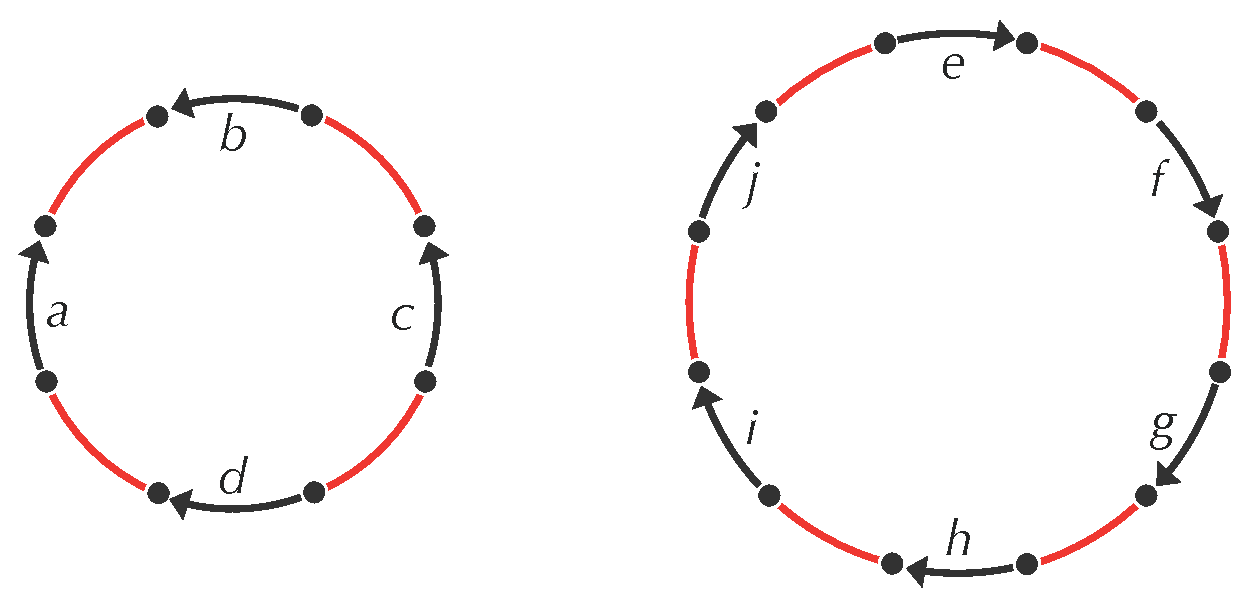
\includegraphics[width = 0.7\textwidth]{images/rearrangements/genome_graph}
\caption{A genome with two circular chromosomes, $(+a$ $-b$ $-c$ $+d)$ and $(+e$ $+f$ $+g$ $+h$ $+i$ $+j)$.  Black directed edges represent synteny blocks, and red undirected edges connect adjacent synteny blocks. A circular chromosome with $n$ elements can be written in $2n$ different ways; the chromosome on the left can be written as $(+a$ $-b$ $-c$ $+d)$, $(-b$ $-c$ $+d$ $+a)$, $(-c$ $+d$ $+a$ $-b)$, $(+d$ $+a$ $-b$ $-c)$, $(-a$ $-d$ $+c$ $+b)$  $(-d$ $+c$ $+b$ $-a)$, $(+c$ $+b$ $-a$ $-d)$, and $(+b$ $-a$ $-d$ $+c)$.}
\label{fig:genome_graph}
\end{figure}

\vspace{\baselineskip}

\begin{qbox}[
Let $P$ and $Q$ be genomes consisting of linear chromosomes, and let $P^{*}$ and $Q^{*}$ be the circularized versions of these genomes. Can you convert a given series of  reversals/translocations/fusions/fissions transforming $P$ into $Q$ into a series of rearrangements transforming $P^{*}$ into $Q^{*}$?  What about the reverse operation --- can you convert a series of rearrangements transforming $P^{*}$ into $Q^{*}$ into a series of rearrangements transforming $P$ into $Q$?
]\end{qbox}

\vspace{-0.5\baselineskip}

\phantomsection
\subsection{2-breaks}
\label{subsec:two-breaks}

We now focus on one of the chromosomes in a multi-chromosomal genome and consider a reversal transforming the circular chromosome $P=(+a$ $-b$ $-c$ $+d)$ into $Q=(+a$ $-b$ $-d$ $+c)$. We can draw $Q$ in a variety of ways, depending on how we choose to arrange its black edges. \autoref{fig:two_equivalent_drawings} shows two such equivalent representations.

\begin{figure}[h]
\mySfFamily
\centering
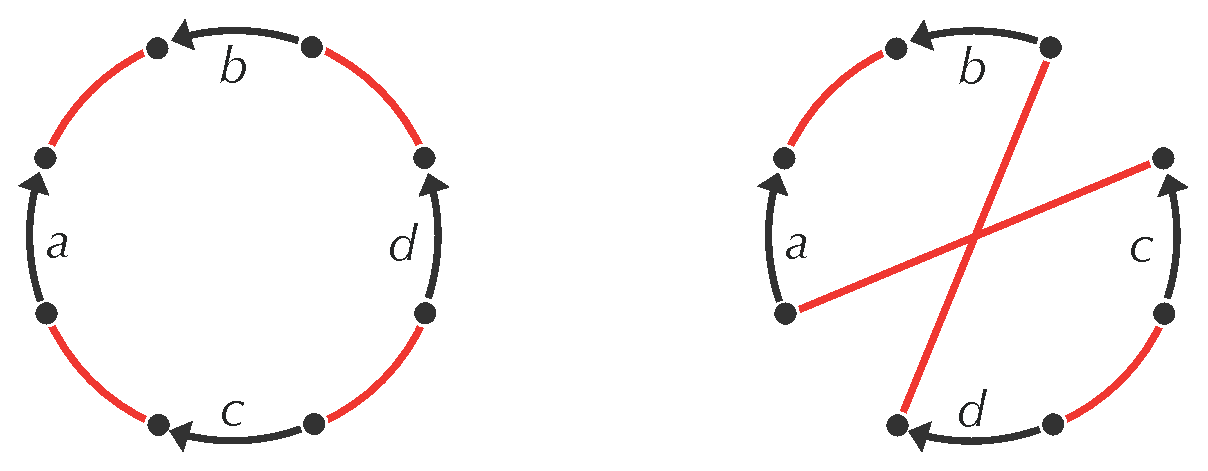
\includegraphics[width = 0.7\textwidth]{images/rearrangements/two_equivalent_drawings}
\caption{Two equivalent drawings of the circular permutation $Q=(+a$ $-b$ $-d$ $+c)$.}
\label{fig:two_equivalent_drawings}
\end{figure}

Although the first drawing of $Q$ in \autoref{fig:two_equivalent_drawings} is its most natural representation, we will use the second representation because its black edges are arranged around the circle in exactly the same order as they appear in the natural representation of $P=(+a$ $-b$ $-c$ $+d)$.  As illustrated in \autoref{fig:genome_reversal}, keeping the black edges fixed allows us to visualize the effect of the reversal.  As you can see, the reversal deletes (``breaks'') two red edges in $P$ (connecting $b$ to $c$ and $d$ to $a$) and replaces them with two new red edges (connecting $b$ to $d$ and $c$ to $a$).\\

\begin{figure}[h]
\mySfFamily
\centering
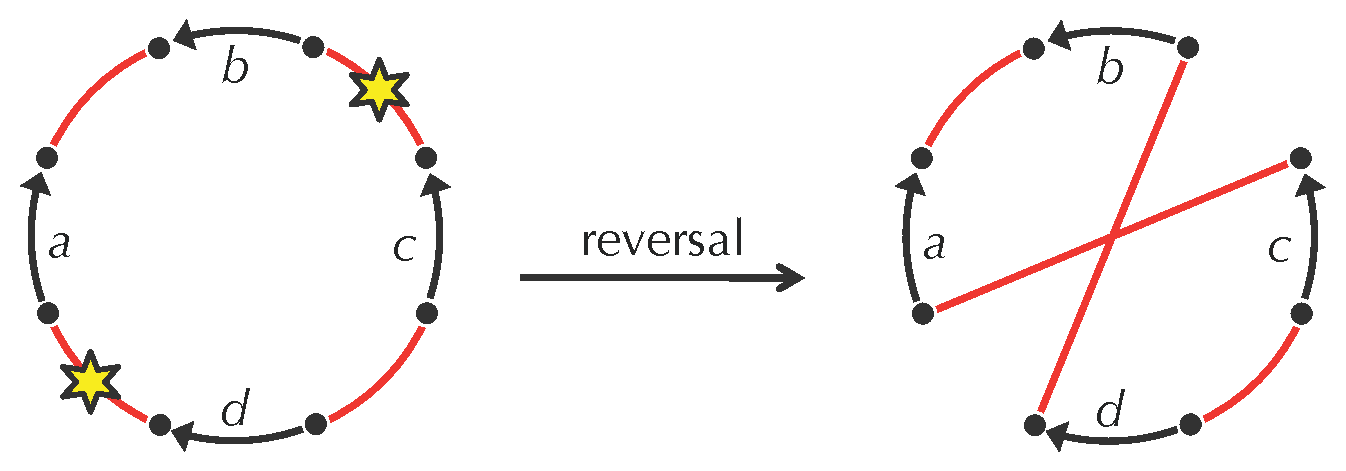
\includegraphics[width = 0.8\textwidth]{images/rearrangements/genome_reversal}
\caption{A reversal transforms $P=(+a$ $-b$ $-c$ $+d)$ into $Q=(+a$ $-b$ $-d$ $+c)$.  We have arranged the black edges of $Q$ so that they have the same orientation and position as the black edges in the natural representation of $P$.  The reversal can be viewed as deleting the two red edges labeled by stars and replacing them with two new red edges on the same four nodes.}
\label{fig:genome_reversal}
\end{figure}

\autoref{fig:fission_and_fusion} illustrates a fission of genome $P=(+a$ $-b$ $-c$ $+d)$ into $Q = (+a$ $-b) (-c$ $+d)$; reversing this operation corresponds to a fusion of the two chromosomes of $Q$ to yield $P$. Both the fusion and the fission operations, like the reversal, correspond to deleting two edges in one genome and replacing them with two new edges in the other genome.

\begin{figure}[h]
\mySfFamily
\centering
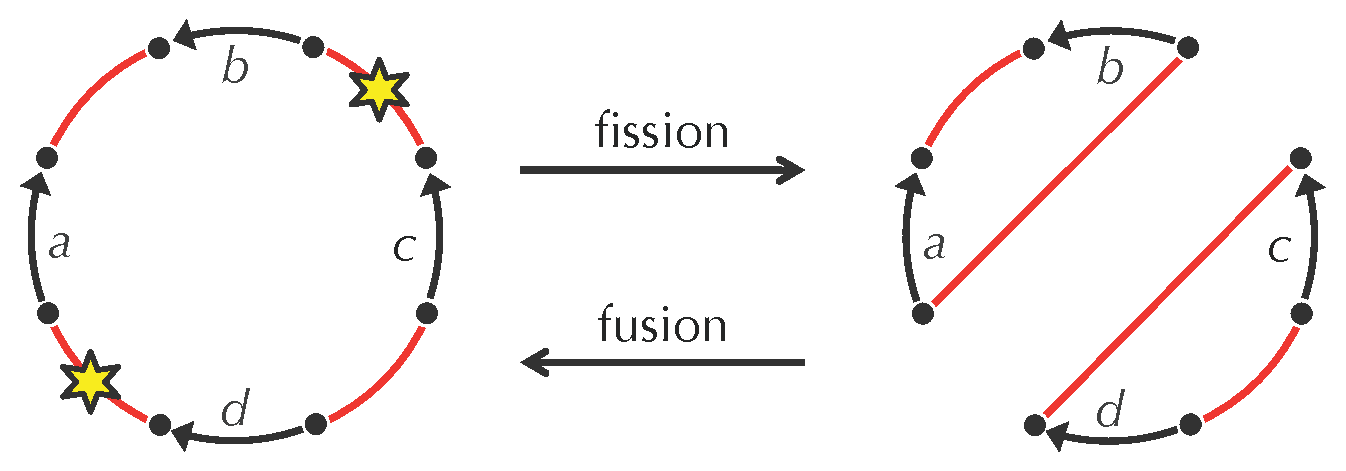
\includegraphics[width = 0.8\textwidth]{images/rearrangements/fission_and_fusion}
\caption{A fission of the single chromosome $P = (+a$ $-b$ $-c$ $+d)$ into the genome $Q = (+a$ $-b)(-c$ $+d)$.  We have again arranged the black edges of $Q$ so that they have the same position and orientation as in the natural representation of $P$.  The inverse operation is a fusion, transforming the two chromosomes of $Q$ into a single chromosome by breaking two red edges of $Q$ and replacing them with two other edges.}
\label{fig:fission_and_fusion}
\end{figure}

A translocation involving two linear chromosomes can also be mimicked by circularizing these chromosomes and then replacing two red edges with two different red edges, as shown in \autoref{fig:translocation}. We have therefore found a common theme uniting the four different types of rearrangements. They all can be viewed as breaking two red edges of the genome graph and replacing them with two new colored edges on the same four nodes.  For this reason, we define the general operation on the genome graph in which two red edges are replaced with two new red edges on the same four nodes as a \textdef{2-break}.

\begin{figure}[h]
\mySfFamily
\centering
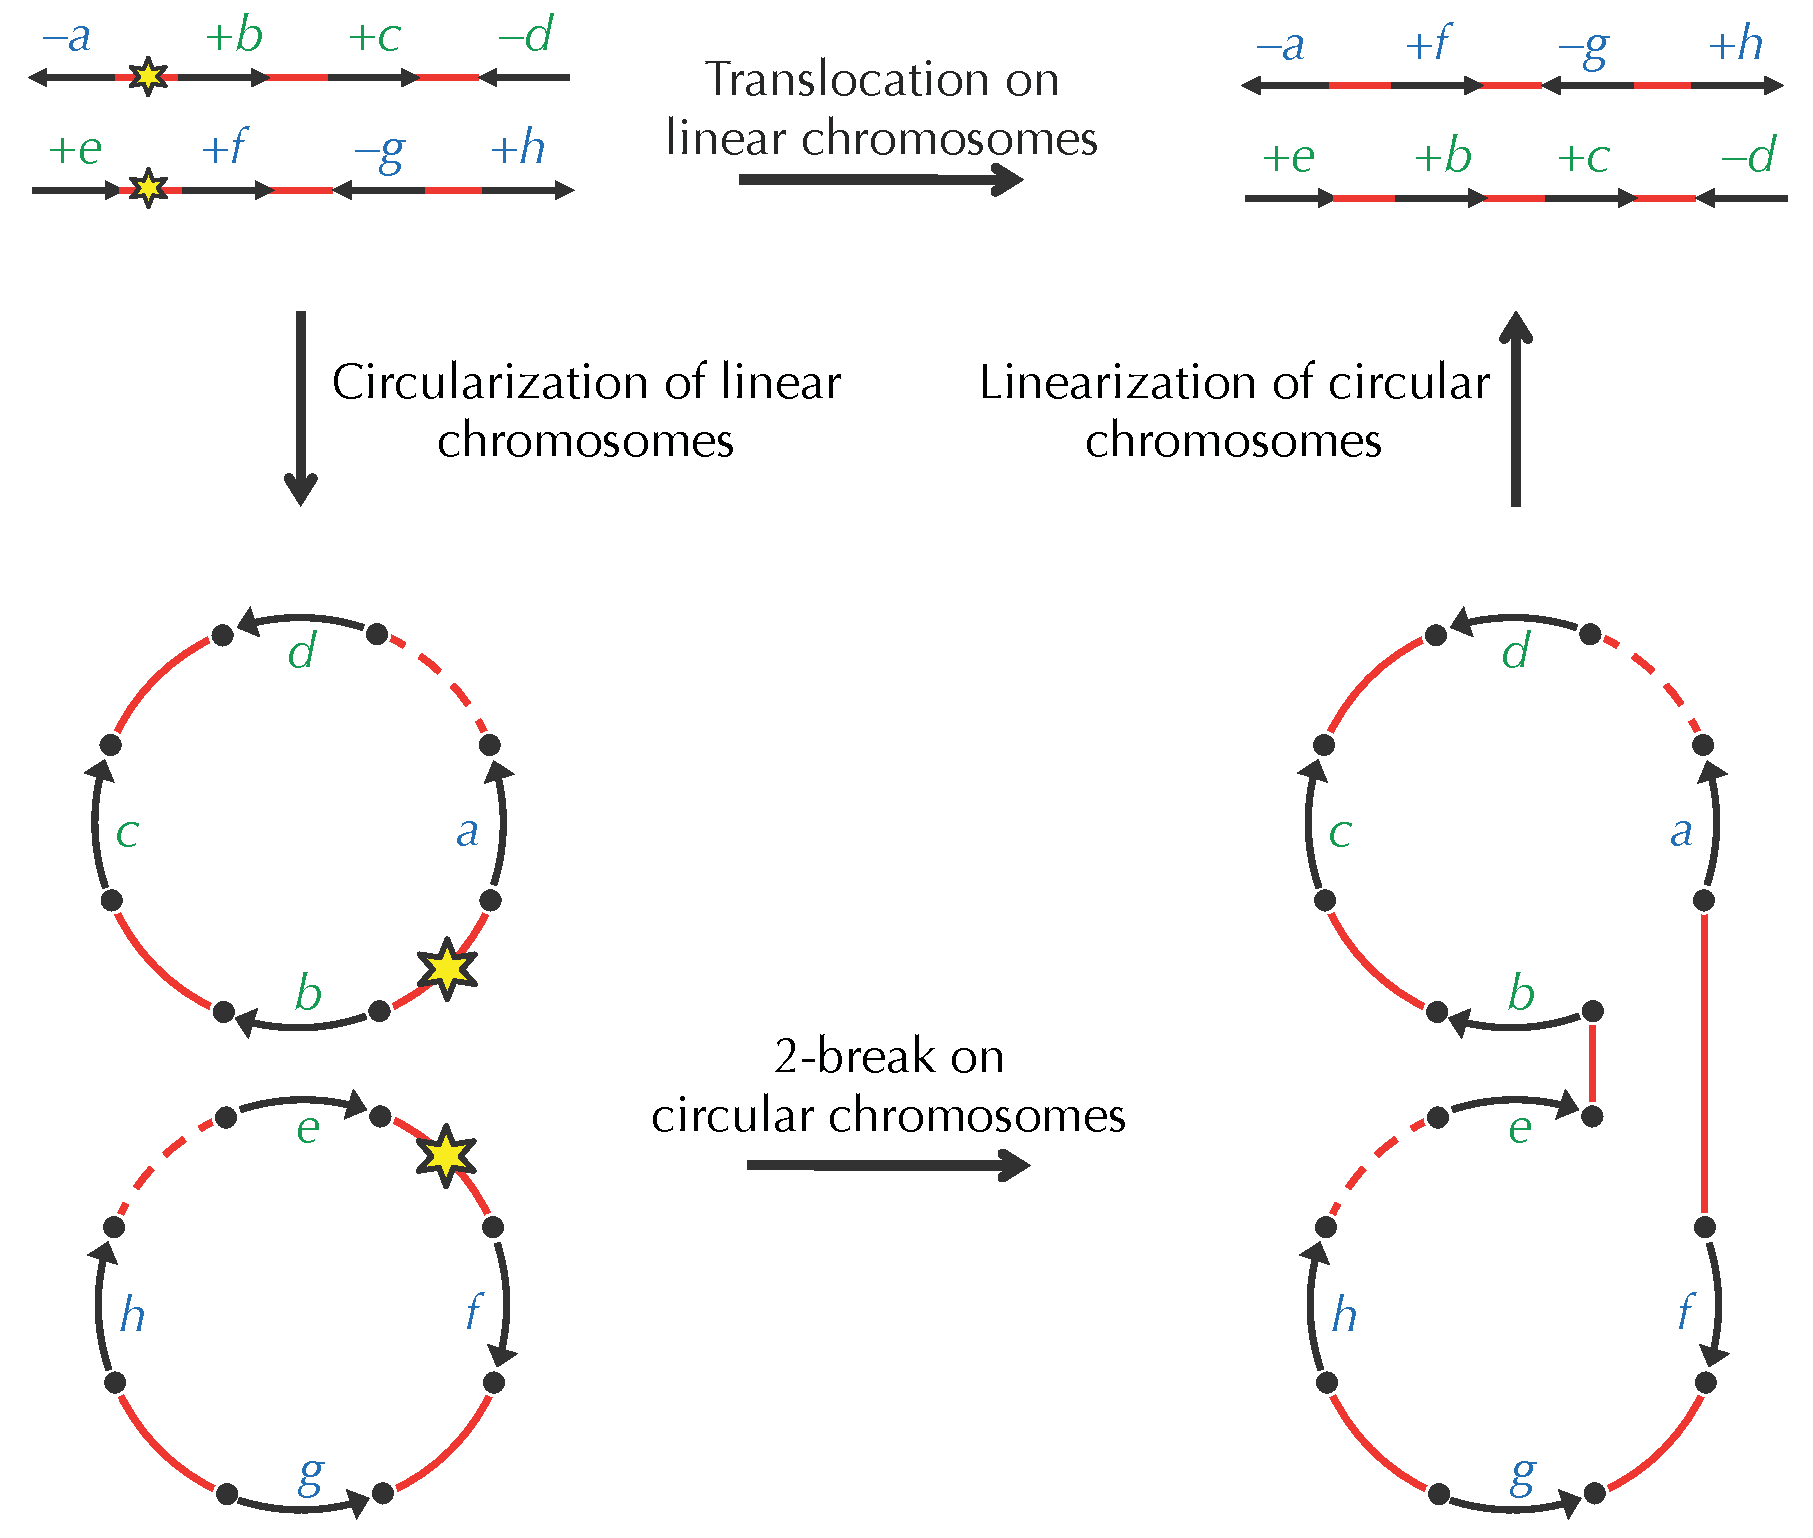
\includegraphics[width = 0.856\textwidth]{images/rearrangements/translocation}
\caption{A translocation of linear chromosomes $(\MathBlue{-a}$ $\MathGreen{+b}$ $\MathGreen{+c}$ $\MathGreen{-d})$  and  $(\MathGreen{+e}$ $\MathBlue{+f}$ $\MathBlue{-g}$ $\MathBlue{+h})$ transforms them into linear chromosomes $(\MathBlue{-a}$ $\MathBlue{+f}$ $\MathBlue{-g}$ $\MathBlue{+h})$ and $(\MathGreen{+e}$ $\MathGreen{+b}$ $\MathGreen{+c}$ $\MathGreen{-d})$. This translocation can also be accomplished by first circularizing the chromosomes, then applying a 2-break to the new chromosomes, and finally converting the resulting circular chromosomes into two linear chromosomes.}
\label{fig:translocation}
\end{figure}

We would like to find a shortest sequence of 2-breaks transforming genome $P$ into genome $Q$, and we refer to the number of operations in this shortest sequence as the \textdef{2-break distance} between $P$ and $Q$, denoted $d(P,Q)$.\\

\begin{problem}[2-Break Distance Problem]{Find the 2-break distance between two genomes.}{Two genomes with circular chromosomes on the same set of synteny blocks.}{The 2-break distance between these genomes.}
\end{problem}

\noindent To compute the 2-break distance, we will return to the notion of breakpoints to construct a graph for comparing two genomes.\\

\phantomsection
\FloatBarrier
\section{Breakpoint Graphs}
\label{sec:breakpoint_graphs}

Consider the genomes $\red{P}=(+a$ $-b$ $-c$ $+d)$ and $\blue{Q} =(+a$ $+c$ $+b$ $-d)$ (\autoref{fig:breakpoint_graph}, left). Note that we have used red for the colored edges of $\red{P}$ and blue for the colored edges of $\blue{Q}$. As before, we rearrange the black edges of $\blue{Q}$ so that they are arranged exactly as in $\red{P}$ (\autoref{fig:breakpoint_graph}, middle). If we superimpose the graphs of $\red{P}$ and $\blue{Q}$, then we obtain the tri-colored \textdef{breakpoint graph} $\textfunc{BreakpointGraph}(\red{P}, \blue{Q})$ (\autoref{fig:breakpoint_graph}, right).

\begin{figure}[h]
\mySfFamily
\centering
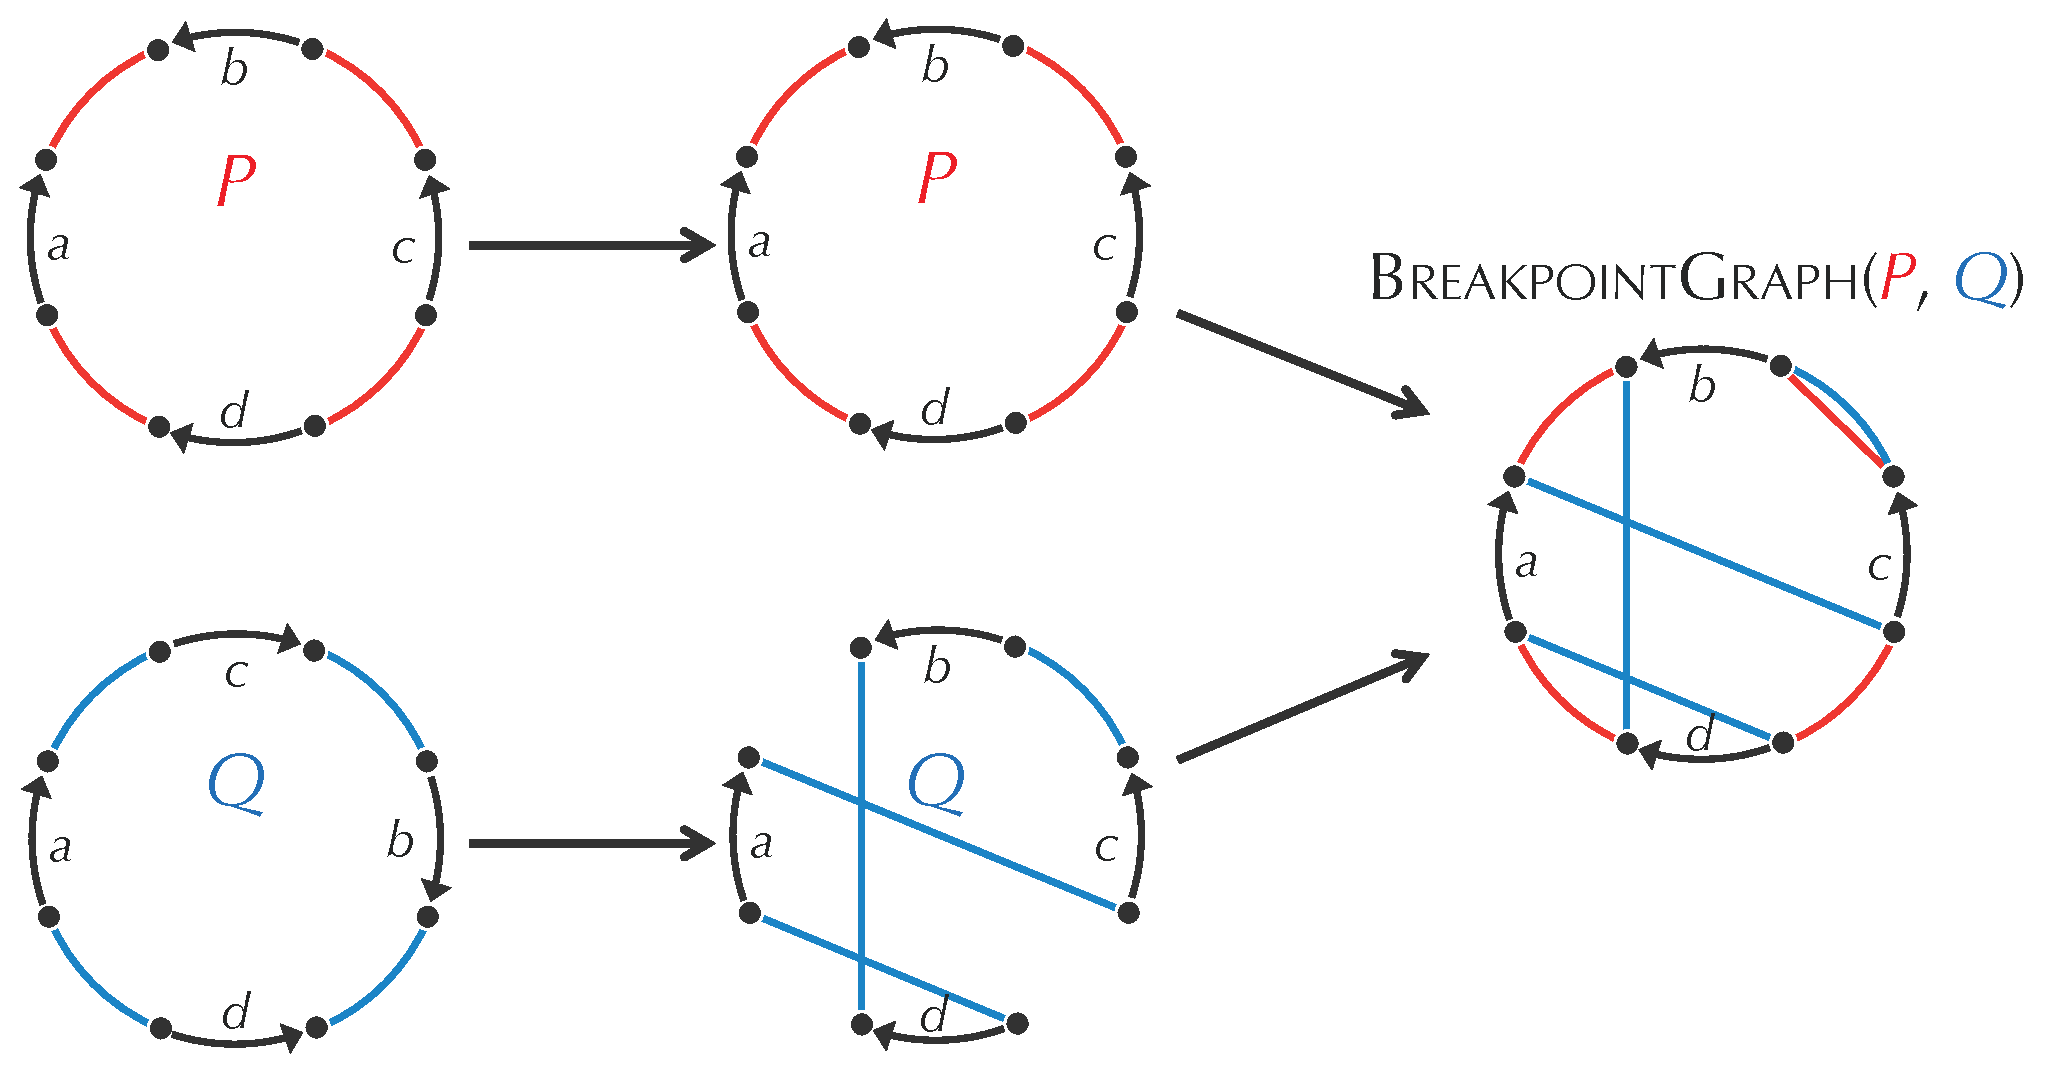
\includegraphics[width = 0.856\textwidth]{images/rearrangements/breakpoint_graph}
\caption{(Left) A red-black genome $\red{P} = (+a ~{-b} ~ {-c} ~ +d)$ and a blue-black genome $\blue{Q} = (+a ~ +c ~ +b ~ {-d})$. (Middle) Rearranging the black edges of $\blue{Q}$ so that they are arranged the same as in $\red{P}$. (Right) The breakpoint graph $\textfunc{BreakpointGraph}(\red{P}, \blue{Q})$, formed by superimposing the graphs of $\red{P}$ and $\blue{Q}$.}
\label{fig:breakpoint_graph}
\end{figure}

Note that the red and black edges in the breakpoint graph form genome $\red{P}$, and the blue and black edges form genome $\blue{Q}$. Moreover, the red and blue edges in the breakpoint graph form a collection of red-blue alternating cycles.\\

\begin{qbox}[
Prove that the red and blue edges in any breakpoint graph form alternating cycles.  Hint: How many red and blue edges meet at each node of the breakpoint graph?
]\end{qbox}

\noindent We denote the number of red-blue alternating cycles in $\textfunc{BreakpointGraph}(\red{P}, \blue{Q})$ as $\textfunc{Cycles}(\red{P}, \blue{Q})$. For $\red{P}=(+a$ $-b$ $-c$ $+d)$ and $\blue{Q} = (+a$ $+c$ $+b$ $-d)$, $\textfunc{Cycles}(\red{P}, \blue{Q}) = 2$, as shown in \autoref{fig:breakpoint_graph_alternating_cycles} (left). In what follows, we will be focusing on the red-blue alternating cycles in breakpoint graphs and often omit the black edges.

\begin{figure}[h]
\mySfFamily
\centering
\begin{tabular}{c @{\hskip 5em} c}
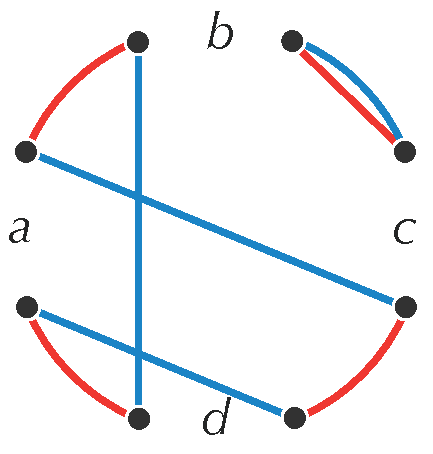
\includegraphics[width = 0.2\textwidth]{images/rearrangements/breakpoint_graph_alternating_cycles} & 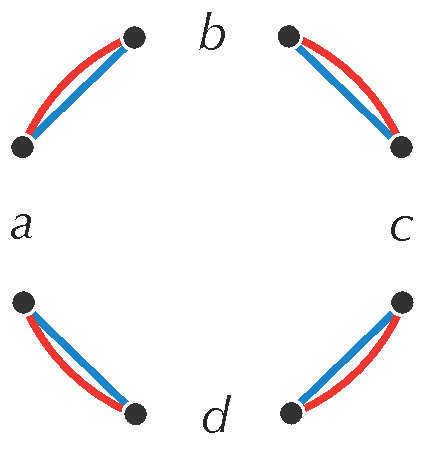
\includegraphics[width = 0.2\textwidth]{images/rearrangements/trivial_breakpoint_graph}
\end{tabular}
\caption{(Left) The red-blue alternating cycles in $\textfunc{BreakpointGraph}(\red{P}, \blue{Q})$ for $\red{P}=(+a$ $-b$ $-c$ $+d)$ and $\blue{Q} = (+a$ $+c$ $+b$ $-d)$. (Right) The trivial breakpoint graph $\textfunc{BreakpointGraph}(\red{P}, \blue{P})$, formed by two copies of the genome $P = (+a$  $-b$ $-c$ $+d)$. The breakpoint graph of \emph{any} genome with itself consists only of trivial (i.e., length 2) alternating cycles.}
\label{fig:breakpoint_graph_alternating_cycles}
\end{figure}

Although \autoref{fig:breakpoint_graph} illustrates the construction of the breakpoint graph for single-chromosomal genomes, the breakpoint graph can be constructed for genomes with multiple chromosomes in exactly the same way (\autoref{fig:breakpoint_graph_multiple_chromosomes}).\\

\begin{figure}[h]
\mySfFamily
\centering
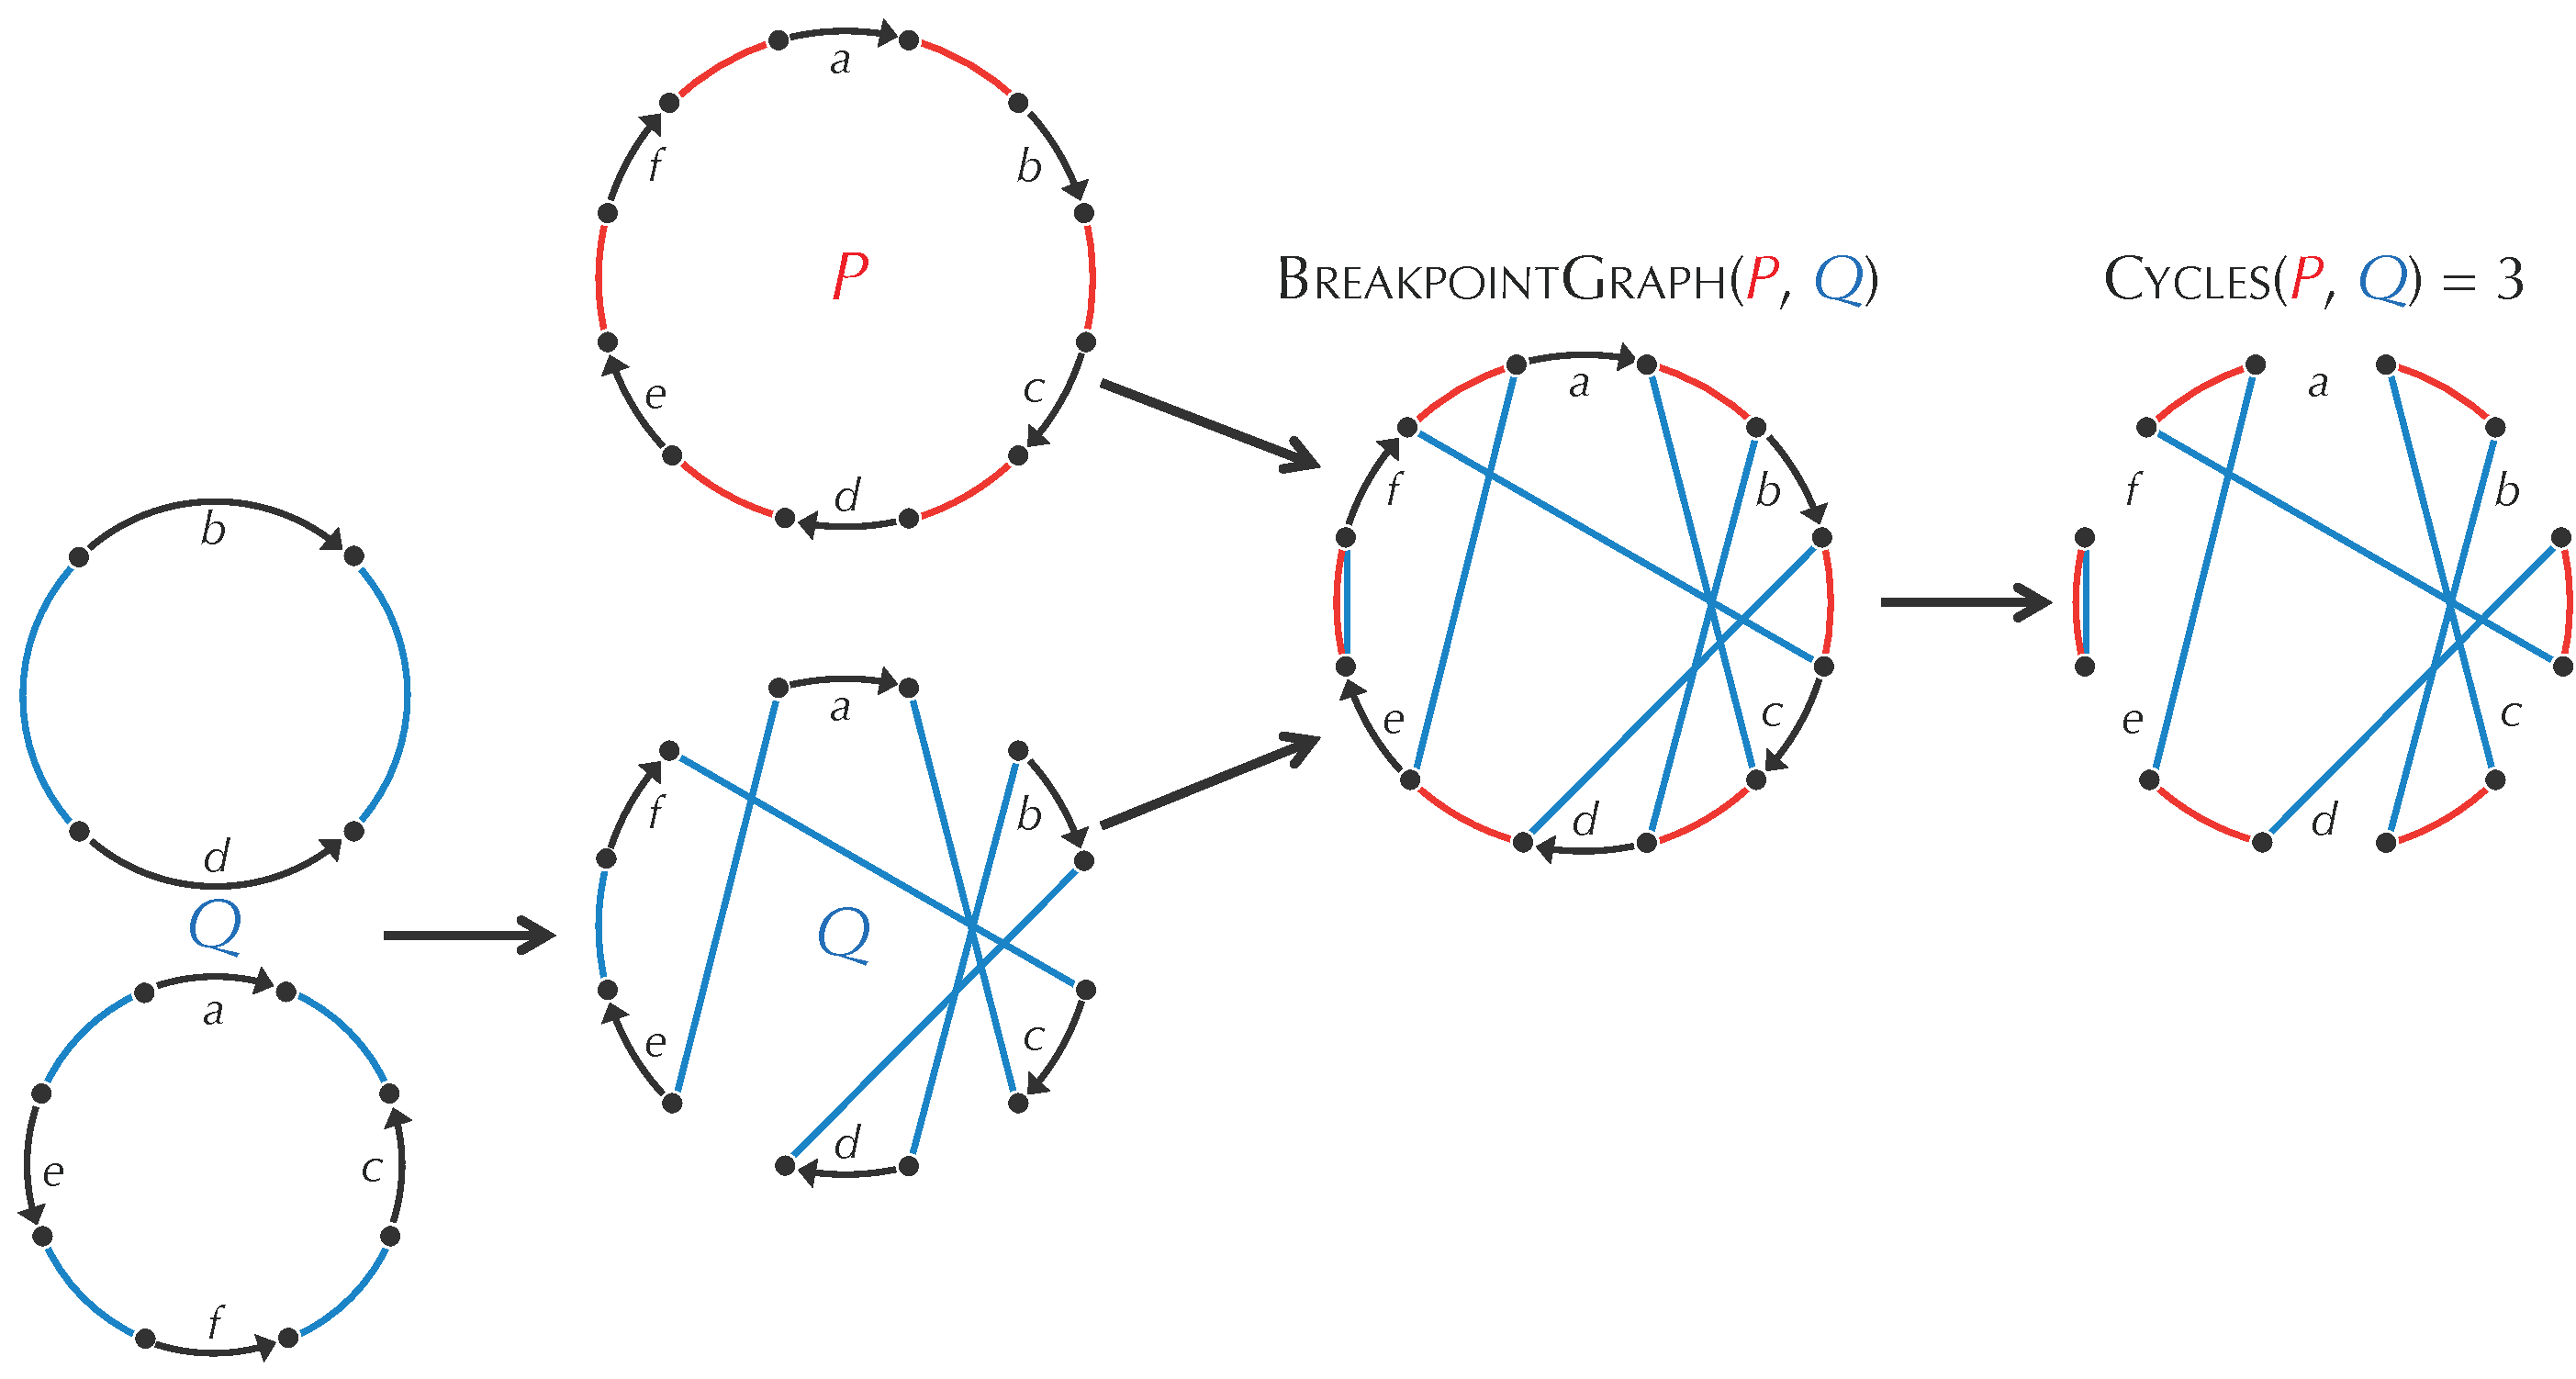
\includegraphics[width = 0.856\textwidth]{images/rearrangements/breakpoint_graph_multiple_chromosomes}
\caption{The construction of $\textfunc{BreakpointGraph}(\red{P}, \blue{Q})$ for the unichromosomal genome $\red{P} = (+a$ $+b$ $+c$ $+d$ $+e$ $+f)$ and the two-chromosome genome $\blue{Q} = (+a$  $-c$ $-f$ $-e)(+b$ $-d)$. At the bottom, to illustrate the construction of the breakpoint graph, we first rearrange the black edges of $\blue{Q}$ so that they are drawn the same as in $\red{P}$.}
\label{fig:breakpoint_graph_multiple_chromosomes}
\end{figure}

\begin{qbox}[
Given genome $\red{P}$, which genome $\blue{Q}$ maximizes $\textfunc{Cycles}(\red{P}, \blue{Q})$?
]\end{qbox}

\vspace{-0.5\baselineskip}

\noindent We denote the number of synteny blocks shared by genomes $\red{P}$ and $\blue{Q}$ as $\textfunc{Blocks}(\red{P}, \blue{Q})$.  As shown in \autoref{fig:breakpoint_graph_alternating_cycles} (right), when $\red{P}$ and $\blue{Q}$ are identical, their breakpoint graph consists of $\textfunc{Blocks}(\red{P}, \blue{Q})$  cycles of length 2, each containing one red and one blue edge. We refer to cycles of length 2 as \textdef{trivial cycles} and the breakpoint graph formed by identical genomes as the \textdef{trivial breakpoint graph}.

%\begin{figure}[h]
%\mySfFamily
%\centering
%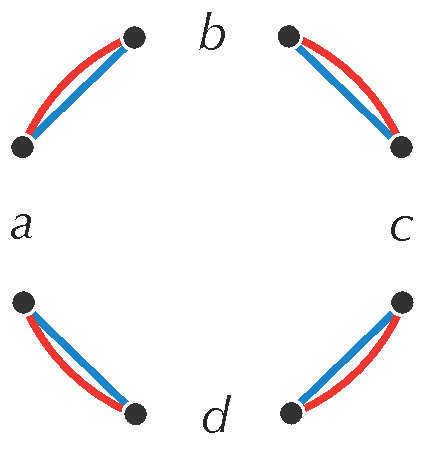
\includegraphics[width = 0.2\textwidth]{images/rearrangements/trivial_breakpoint_graph}
%\caption{The trivial breakpoint graph $\textfunc{BreakpointGraph}(\red{Q}, \blue{Q})$ formed by two copies of the genome $Q = (+a$  $-b$ $-c$ $+d)$.}
%\label{fig:trivial_breakpoint_graph}
%\end{figure}

You are likely wondering how the breakpoint graph is useful. We can view a 2-break transforming $\red{P}$ into $\red{P'}$ as an operation on $\textfunc{BreakpointGraph}(\red{P}, \blue{Q})$ that yields $\textfunc{BreakpointGraph}(\red{P'}\hspace{-0.1em}, \blue{Q})$ (\autoref{fig:2_break_breakpoint_graph}).

By extension, we can view a series of 2-breaks transforming $\red{P}$ into $\blue{Q}$ as a series of 2-breaks transforming $\textfunc{BreakpointGraph}(\red{P}, \blue{Q})$ into $\textfunc{BreakpointGraph}(\red{Q}, \blue{Q})$, the trivial breakpoint graph (\autoref{fig:2_break_series}).  \autoref{fig:2_break_series_example} illustrates a transformation of a breakpoint graph with $\textfunc{Cycles}(\red{P}, \blue{Q}) = 2$ into a trivial breakpoint graph with $\textfunc{Cycles}(\red{Q}, \blue{Q}) = 4$ using two 2-breaks.\par

\begin{figure}[h]
\mySfFamily
\centering
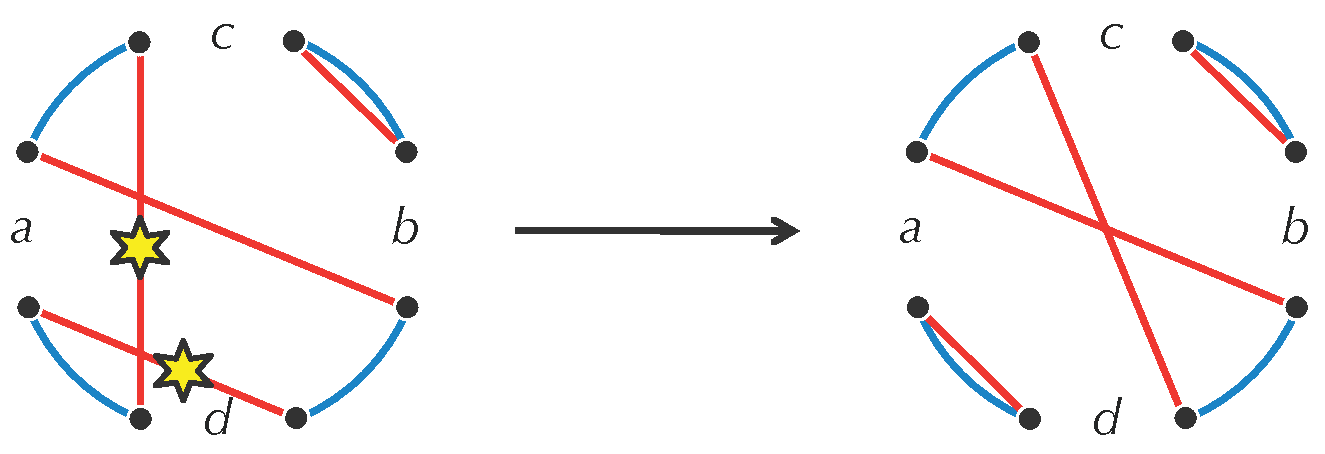
\includegraphics[width = 0.6\textwidth]{images/rearrangements/2-break_breakpoint_graph}
\caption{A 2-break transforming genome $\red{P}$ into genome $\red{P'}$ also transforms $\textfunc{BreakpointGraph}(\red{P}, \blue{Q})$ into  $\textfunc{BreakpointGraph}(\red{P'}\hspace{-0.1em}, \blue{Q})$ for any permutation $\blue{Q}$.}
\label{fig:2_break_breakpoint_graph}
\end{figure}

\begin{figure}[h]
\mySfFamily
\centering
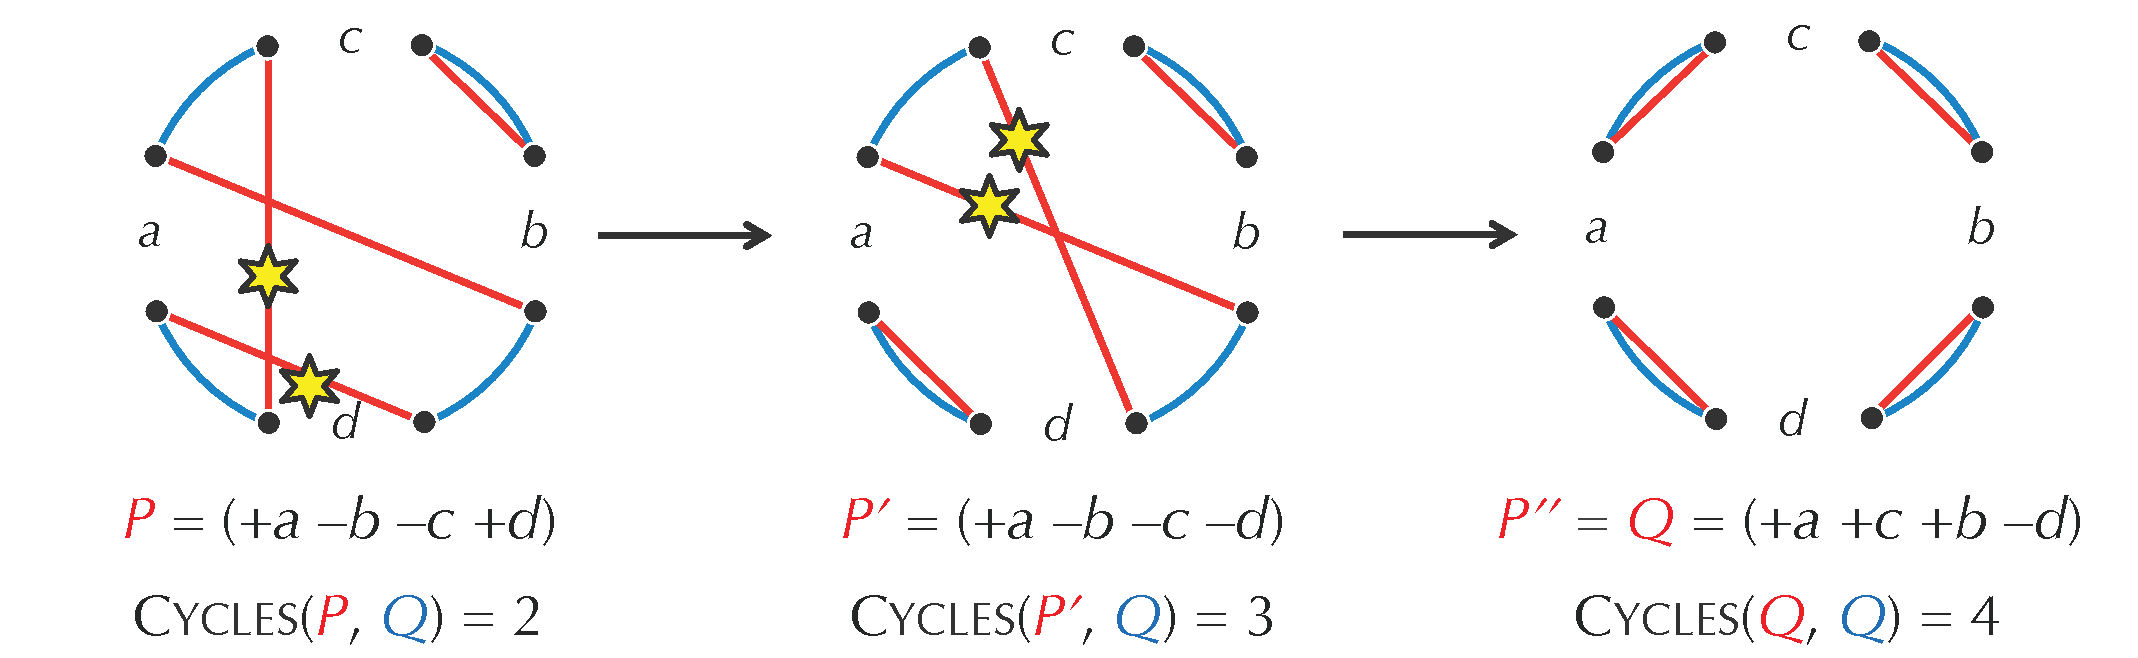
\includegraphics[width = 0.856\textwidth]{images/rearrangements/2-break_series}
\caption{Every 2-break transformation of $\red{P}$ into $\blue{Q}$ corresponds to a transformation of $\textfunc{BreakpointGraph}(\red{P}, \blue{Q})$ into $\textfunc{BreakpointGraph}(\red{Q}, \blue{Q})$. In the example shown, the number of red-blue cycles in the graph increases from $\textfunc{Cycles}(\red{P}, \blue{Q}) = 2$ to $\textfunc{BreakpointGraph}(\red{Q}, \blue{Q}) = \textfunc{Blocks}(\red{Q}, \blue{Q}) = 4$.}
\label{fig:2_break_series}
\end{figure}

\begin{figure}[h]
\mySfFamily
\centering
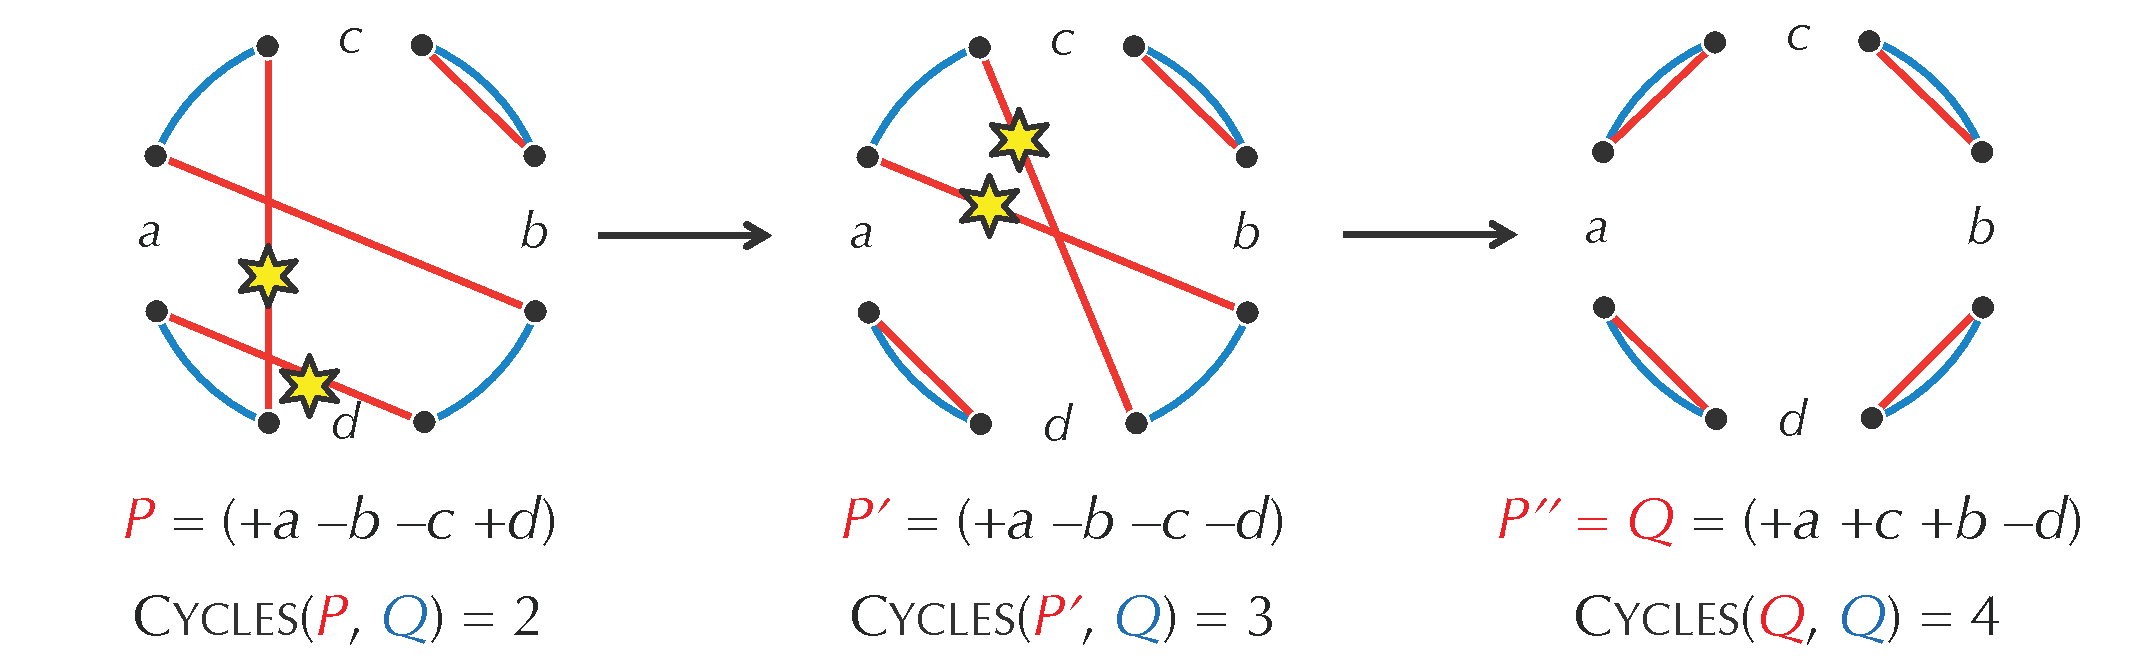
\includegraphics[width = 0.856\textwidth]{images/rearrangements/2-break_series_example}
\caption{The transformation $\red{P} \rightarrow \red{P'} \rightarrow \red{Q}$ induces a transformation of the breakpoint graph $\textfunc{BreakpointGraph}(\red{P}, \blue{Q})$ with 2 alternating cycles into the trivial breakpoint graph.  Stars indicate red edges that are replaced in a 2-break.}
\label{fig:2_break_series_example}
\end{figure}



Since every transformation of $\red{P}$ into $\blue{Q}$ transforms  $\textfunc{BreakpointGraph}(\red{P}, \blue{Q})$ into the trivial breakpoint graph $\textfunc{BreakpointGraph}(\red{Q}, \blue{Q})$, any sorting by 2-breaks increases the number of red-blue cycles by

\begin{center}
$\textfunc{Cycles}(\red{Q}, \blue{Q}) - \textfunc{Cycles}(\red{P}, \blue{Q}) = \textfunc{Blocks}(\red{P}, \blue{Q}) - \textfunc{Cycles}(\red{P}, \blue{Q})$.
\end{center}

\fudgespace

\begin{qbox}[
How much can each individual 2-break contribute to this increase? In other words, if $\red{P'}$ is obtained from $\red{P}$ by a 2-break, how much bigger can $\textfunc{Cycles}(\red{P'}, \blue{Q}) $ be than $\textfunc{Cycles}(\red{P}, \blue{Q})$?
]\end{qbox}

\phantomsection
\FloatBarrier
\section{Computing the 2-Break Distance}
\label{sec:computing_the_2-break_distance}

The Breakpoint Theorem stated that a reversal applied to a linear chromosome $P$ can reduce $\textfunc{Breakpoints}(P)$ by at most 2.  We now prove that a 2-break applied to a multichromosomal genome $P$ can increase $\textfunc{Cycles}(P, Q)$ by at most 1, i.e., for any 2-break transforming $P$ into $P'$, and for any genome $Q$, $\textfunc{Cycles}(P', Q)$ cannot exceed $\textfunc{Cycles}(P, Q) + 1$.

\begin{namedtheorem}[Cycle]
For genomes $P$ and $Q$, any 2-break applied to $P$ can increase $\textfunc{Cycles}(P, Q)$ by at most 1. 
\end{namedtheorem}

\begin{proof}
\autoref{fig:cycle_theorem_proof} presents three cases that illustrate how a 2-break applied to $P$ can affect the breakpoint graph. Each 2-break affects two red edges that either belong to the same cycle or to two different cycles in $\textfunc{BreakpointGraph}(P, Q)$. In the former case, the 2-break either does not change $\textfunc{Cycles}(P, Q)$, or it increases it by 1. In the latter case, it decreases $\textfunc{Cycles}(P, Q)$ by 1.
\end{proof}

\begin{figure}[h]
\mySfFamily
\centering
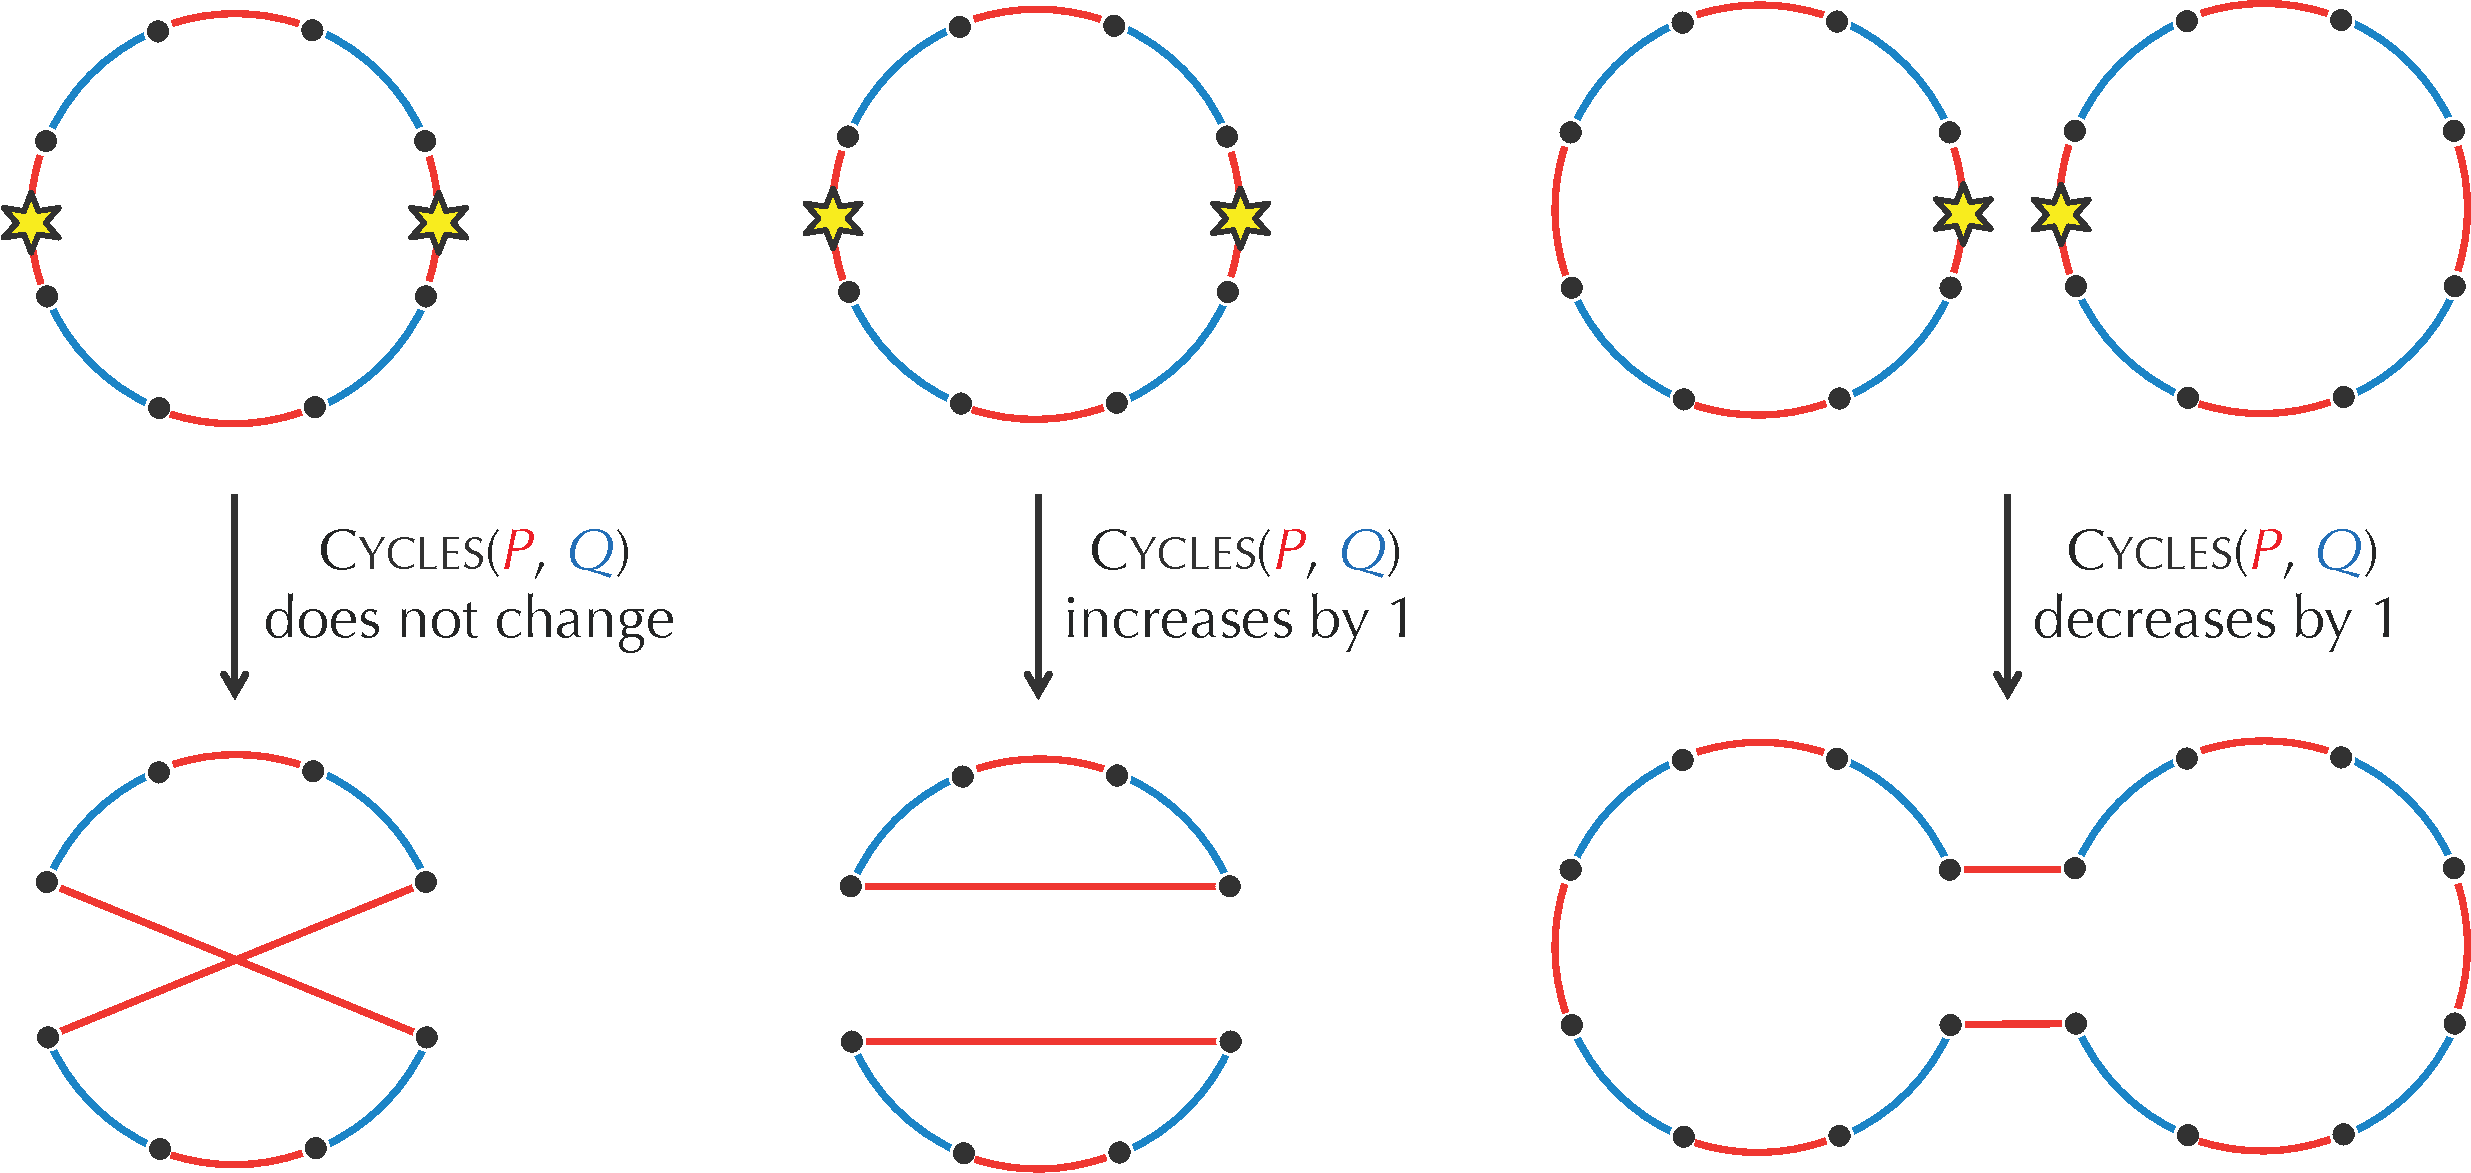
\includegraphics[width = 0.856\textwidth]{images/rearrangements/cycle_theorem_proof}
\caption{Three cases illustrating how a 2-break can affect the breakpoint graph.}
\label{fig:cycle_theorem_proof}
\end{figure}

Although the preceding proof is short and intuitive, it is not a formal proof, but rather an invitation to examine \autoref{fig:cycle_theorem_proof}. If you are interested in a more rigorous mathematical argument, please read the next proof.

\begin{proof}
A 2-break adds 2 new red edges and thus forms at most \textbf{2} new cycles (containing two new red edges) in $\textfunc{BreakpointGraph}(P, Q)$.  At the same time, it breaks 2 red edges and thus removes at least \textbf{1} old cycle (containing two old edges) from $\textfunc{BreakpointGraph}(P, Q)$.  Thus, the number of red-blue cycles in the breakpoint graph increases by at most $\textbf{2} - \textbf{1} = 1$, implying that $\textfunc{Cycles}(P, Q)$ increases by at most 1.
\end{proof}

Recall that there are permutations for which the number of breakpoints cannot be reduced, a fact that defeated our hopes for a greedy algorithm for sorting by reversals that reduces the number of breakpoints at each step. In the case of 2-breaks (on genomes with circular chromosomes), we now know that each 2-break can increase $\textfunc{Cycles}(P, Q)$ by at most 1. But is it \emph{always} possible to find a 2-break that increases $\textfunc{Cycles}(P, Q)$ by 1? The answer, perhaps surprisingly, is yes.

\begin{namedtheorem}[2-Break Distance]
The 2-break distance between genomes $P$ and $Q$ is equal to $\textfunc{Blocks}(P, Q) - \textfunc{Cycles}(P, Q)$.
\end{namedtheorem}

\begin{proof}
Recall that every sorting by 2-breaks must increase the number of alternating cycles by $\textfunc{Blocks}(P, Q) - \textfunc{Cycles}(P, Q)$. The Cycle Theorem implies that each 2-break increases the number of cycles in the breakpoint graph by at most 1.  This immediately implies in turn that $d(P, Q)$ is \emph{at least} $\textfunc{Blocks}(P, Q) - \textfunc{Cycles}(P, Q)$. If $P$ is not equal to $Q$, there must be a non-trivial cycle in $\textfunc{Blocks}(P, Q)$, i.e., a cycle with more than 2 edges. As shown in \autoref{fig:cycle_theorem_proof} (middle), any non-trivial cycle in the breakpoint graph can be split into two cycles by a 2-break, implying that we can always find a 2-break increasing the number of red-blue cycles by 1. Therefore, $d(P,Q)$ is equal to $\textfunc{Blocks}(P, Q) - \textfunc{Cycles}(P, Q)$.
\end{proof}

\protect\computationalproblem[2-Break Distance Problem]{0.8}
Armed with this theorem, you should be ready to design an algorithm solving the 2-Break Distance Problem. Furthermore, having proved the formula $d(P,Q) = \textfunc{Blocks}(P, Q) - \textfunc{Cycles}(P, Q)$ for the 2-break distance between genomes with multiple circular chromosomes, we wonder whether we can find an analogous formula for the reversal distance between single linear chromosomes.\par

\vspace{\baselineskip}

\begin{qbox}[
Compute the 2-break distance between the circularized human and mouse X chromosomes. Can you transform a series of 2-breaks for circularized chromosomes into a series of reversals sorting the linear X chromosomes?
]\end{qbox}

\noindent Perhaps surprisingly, a fast algorithm for sorting permutations by reversals does exist, yielding an exact formula for the reversal distance!  Although this sorting algorithm relies on the notion of breakpoints, it is unfortunately too complicated to present here (see \takedetour[Similar Problems with Different Fates]{similar_problems_with_different_fates}).

The breakpoint graph constructed on the 280 human-mouse synteny blocks contains 35 alternating cycles, so that the 2-break distance between these genomes is $280 - 35 = 245$.  Again, we don't know exactly how many 2-breaks happened in the last 75 million years, but we are certain that there were \emph{at least} 245 steps. Remember this fact, since it will prove important in the next section.\\

\phantomsection
\FloatBarrier
\section{Rearrangement Hotspots in the Human Genome}
\label{sec:rearrangement_hotspots_in_the_human_genome}

\phantomsection
\subsection{The Random Breakage Model meets the 2-Break Distance Theorem}
\label{subsec:the_random_breakage_model_meets_the_2-break_distance_theorem}

You have probably anticipated from the beginning of the chapter that we would eventually argue against the Random Breakage Model.  But it may still be unclear to you how the 2-break distance could possibly be used to do so.

\begin{namedtheorem}[Rearrangement Hotspots]
There are rearrangement hotspots in the human \linebreak genome. 
\end{namedtheorem}

\begin{proof}
Recall that if the Random Breakage Model is correct, then $N$ reversals applied to a linear chromosome will produce approximately $2N + 1$ synteny blocks, since the probability is very low that two nearby locations in the genome will be used as the breakage point of more than one reversal. Similarly, $N$ random 2-breaks applied to circular chromosomes will produce $2N$ synteny blocks. Since there are 280 human-mouse synteny blocks, there must have been approximately $\left. 280 \middle/ 2 = 140 \right.$ 2-breaks on the evolutionary path between humans and mice. However, the 2-Break Distance Theorem tells us that there were at least 245 2-breaks on this evolutionary path.\\

\begin{qbox}[
Is $245 \approx 140$?
]\end{qbox}

\vspace{-0.5\baselineskip}

\noindent Since 245 is much larger than 140, we have arrived at a contradiction, implying that one of our assumptions is incorrect! But the only assumption we made in this proof was ``\emph{If the Random Breakage Model is correct\ldots}'' Thus, this assumption must have been wrong.
\end{proof}

This argument, which is not a mathematical proof, is nevertheless logically solid.  It offers an example of a \textdef{proof by contradiction}, in which we begin by assuming the statement that we intend to disprove and then demonstrate how this assumption leads to a contradiction. As a result of the Rearrangement Hotspots Theorem, we conclude that there was breakpoint reuse on the human-mouse evolutionary path.  This breakpoint reuse was extensive, as quantified by the large ratio between the actual 2-break distance and what the 2-break distance would have been under the Random Breakage Model ($\left. 245 \middle/ 140 = 1.75 \right.$).

Of course, our arguments need to be made statistically sound in order to ensure that the discrepancy between the Random Breakage Model's prediction and the 2-break distance is significant.  After all, even though genomes are large, there is still a small chance that randomly chosen 2-breaks might occasionally break a genome more than once in a small interval.  Unfortunately, the necessary statistical analysis is beyond the scope of this chapter.

\phantomsection
\subsection{The Fragile Breakage Model}
\label{subsec:the_fragile_breakage_model}

But wait --- what about Nadeau and Taylor's argument in favor of the Random Breakage Model?  We certainly cannot ignore that the lengths of the human-mouse synteny blocks resemble an exponential distribution.\\

\begin{qbox}[
Can you find anything wrong with Nadeau and Taylor's logic?
]\end{qbox}

\noindent The Nadeau and Taylor argument in favor of the Random Breakage Model exemplifies a classic logic fallacy.  It is true that if breakage is random, then the histogram of synteny block lengths should follow the exponential distribution. But it is a completely different statement to conclude that just because synteny block lengths follow the exponential distribution, breakage must have been random.  The distribution of synteny block lengths certainly provides support for the Random Breakage Model, but it does not prove that it is correct.

Nevertheless, any alternative hypothesis we put forth for the Random Breakage Model must account for the observation that the distribution of synteny block lengths for the human and mouse genomes is approximately exponential.\\

\begin{qbox}[
Can you propose a different model of chromosome evolution that explains rearrangement hotspots and is consistent with the exponential distribution of synteny block lengths?
]\end{qbox}

\noindent The contradiction of the Random Breakage Model led to an alternative \textdef{Fragile Breakage Model} of chromosome evolution, which was proposed in 2003.  This model states that every mammalian genome is a mosaic of long solid regions, which are rarely affected by rearrangements, as well as short \textdef{fragile regions} that serve as rearrangement hotspots and that account only for a small fraction of the genome.  For humans and mice, these fragile regions make up approximately 3\% of the genome.

If we once again follow Occam's razor, then the most reasonable way to allow for exponentially distributed synteny block lengths is if the fragile regions themselves are distributed randomly in the genome. Indeed, \emph{randomly} selecting breakpoints within \emph{randomly} distributed fragile regions is not unlike randomly selecting the endpoints of a rearrangement throughout the entire genome.  Yet although we now have a model that fits our observations, many questions remain. For example, it is unclear where fragile regions are located, or what causes genomic fragility in the first place.\\

\begin{qbox}[
Consider the following statement: ``The exponential distribution of synteny block lengths and extensive breakpoint re-use imply that the Fragile Breakage Model must be true.'' Is this argument logically sound?
]\end{qbox}

\noindent The point we are driving at by asking the preceding question is that we will never be able to prove a scientific theory like the Fragile Breakage Model in the same way that we have proved one of the mathematical theorems in this chapter. In fact, many biological theories are based on arguments that a mathematician would view as fallacious; the logical framework used in biology is quite different from that used in mathematics. To take an historical example, neither Darwin nor anyone else has ever proved that evolution by natural selection is the only --- or even the most likely --- explanation for how life on Earth evolved!

We have already given many reasons to biology professors to send us to Biology 101 boot camp, but now we will probably be rounded up and imprisoned with Intelligent Design proponents. However, not even Darwinism is unassailable; in the 20th Century, this theory was revised into Neo-Darwinism, and there is little doubt that it will continue to evolve.\\

\phantomsection
\FloatBarrier
\section{Epilogue: Synteny Block Construction}
\label{sec:synteny_block_construction}

Throughout our discussion of genome rearrangements, we assumed that we were given synteny blocks in advance.  In this section, we will explain how to construct synteny blocks from genomic sequences.

\phantomsection
\subsection{Genomic dot-plots}
\label{subsec:genomic_dot-plots}

Biologists sometimes visualize repeated $k$-mers within a string as a collection of points in the plane; a point with coordinates $(x,y)$ represents identical $k$-mers occurring at positions $x$ and $y$ in the string.  The top panels in \autoref{fig:genomic_dot_plots} present two of these \textdef{genomic dot plots}.  Of course, since DNA is double-stranded, we should expand the notion of repeated $k$-mers to account for repeats occurring in the complementary strand. In the bottom left panel of \autoref{fig:genomic_dot_plots}, blue points $(x,y)$ indicate that the $k$-mers starting at positions $x$ and $y$ of the string are reverse complementary.

\phantomsection
\subsection{Finding shared \emph{k}-mers}
\label{subsec:finding_shared_k-mers}

Recalling that a synteny block is defined by many similar genes occurring in the same order in two genomes, let's first find the positions of all $k$-mers that are shared by the human and mouse X chromosomes. If we choose $k$ to be sufficiently large (e.g., $k = 30$), then it is rather unlikely that shared $k$-mers represent spurious similarities. A more likely explanation is that they come from related genes (or shared repeats) in the human and mouse genomes.

Formally, we say that a $k$-mer is \textdef{shared} by two genomes if either the $k$-mer or its reverse complement appears in each genome. Below are four pairs of 3-mers (shown in bold) that are shared by \textnucl{AAACTCATC} and \textnucl{TTTCAAATC}; note that the second pair of 3-mers are reverse complements of each other.

\begin{figure}[p]
\mySfFamily
\centering
\begin{tabular}{c @{\hskip 2em} c}
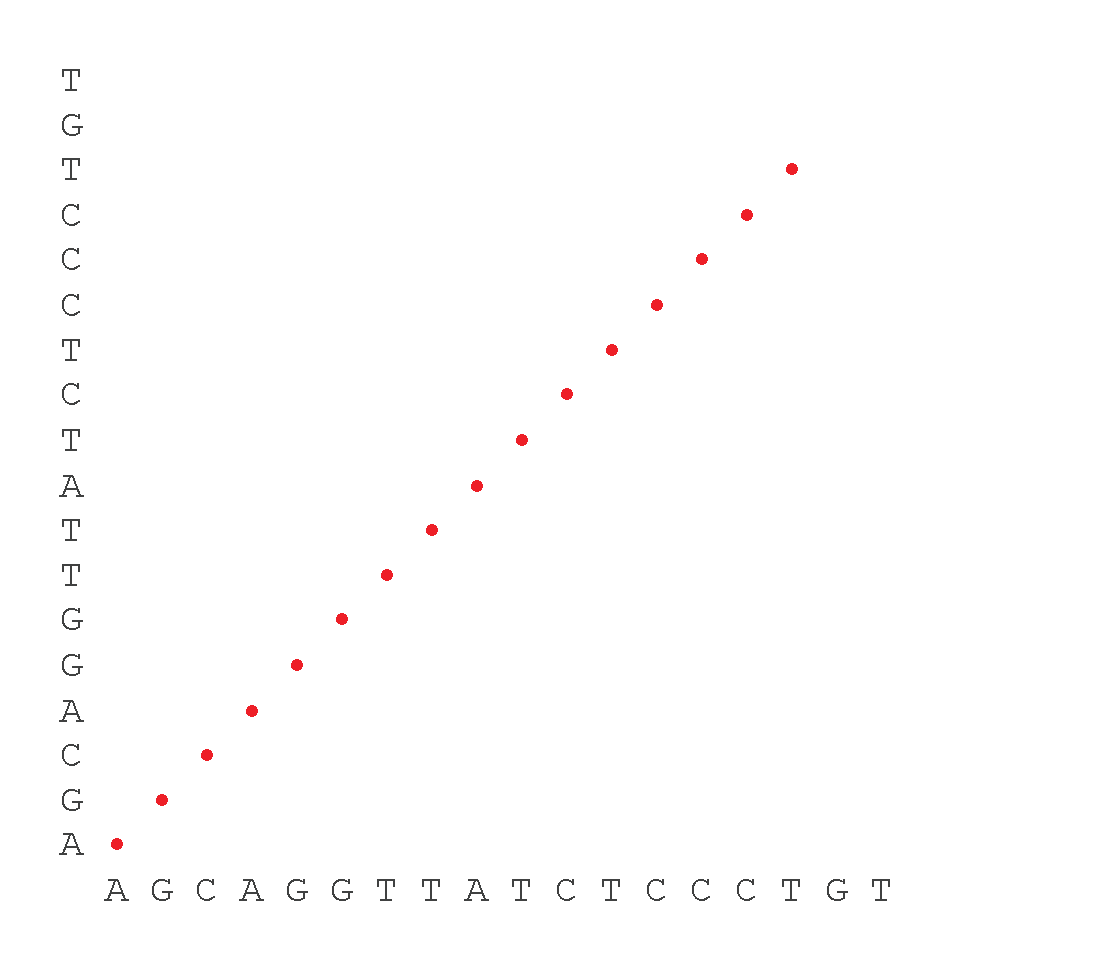
\includegraphics[width = 0.4\textwidth]{images/rearrangements/genomic_dot_plots-1} & 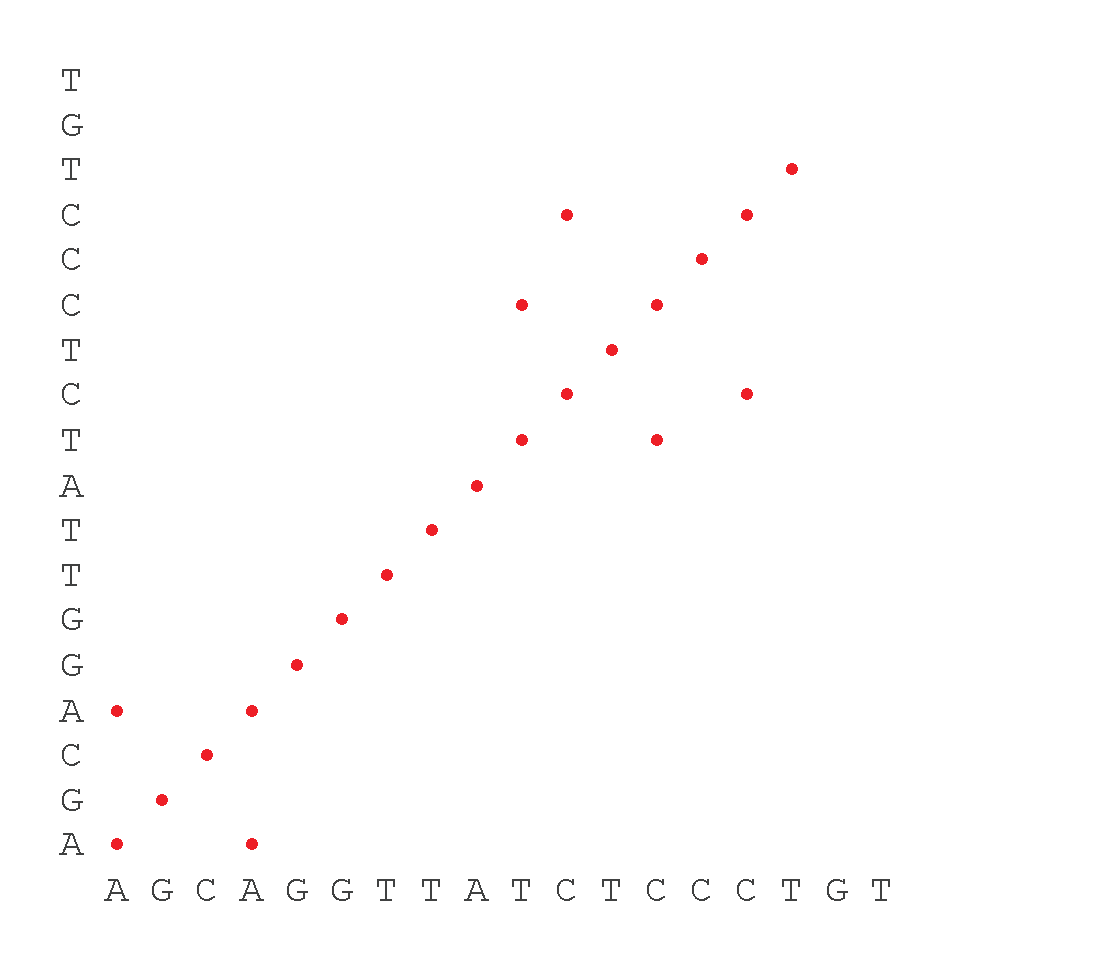
\includegraphics[width = 0.4\textwidth]{images/rearrangements/genomic_dot_plots-2}\\[3ex]
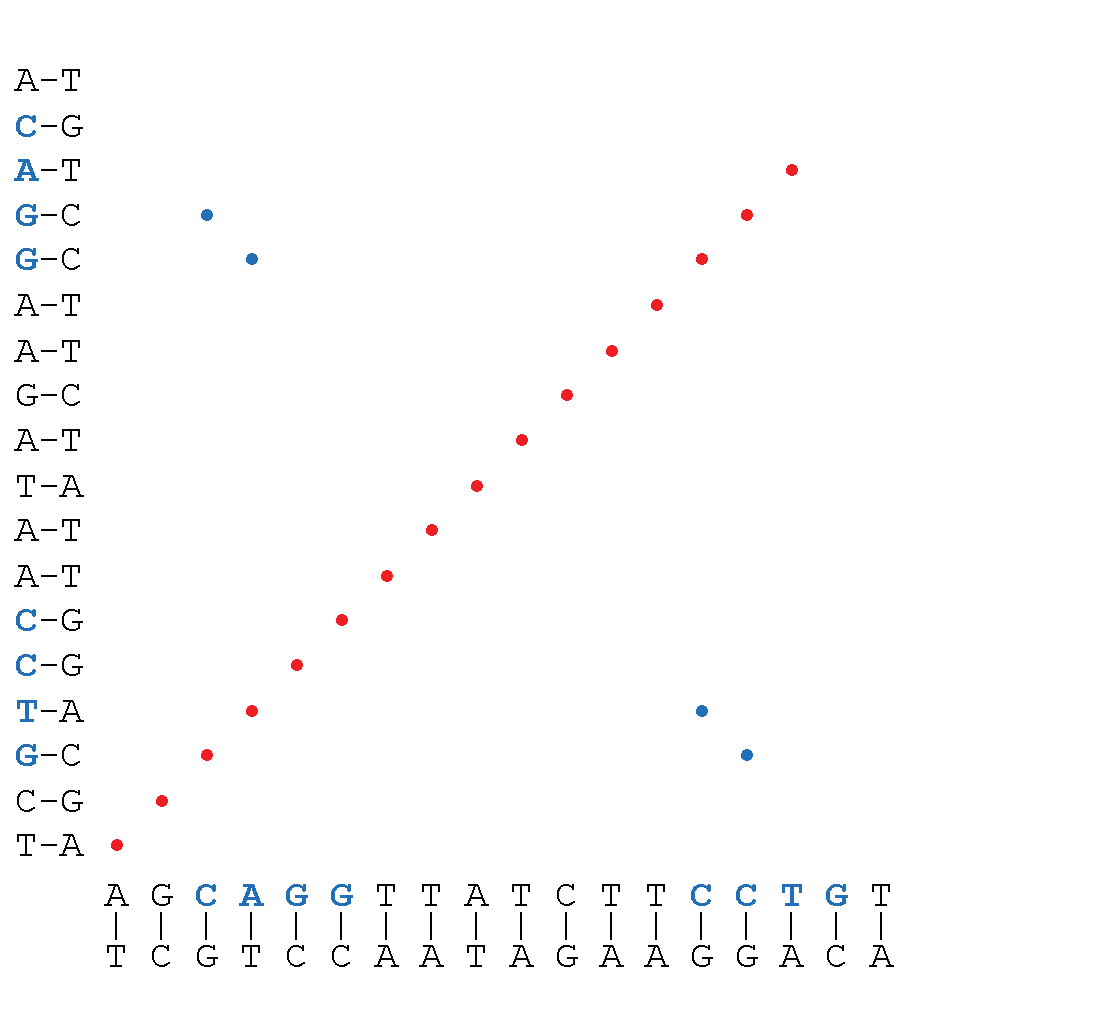
\includegraphics[width = 0.4\textwidth]{images/rearrangements/genomic_dot_plots-3} & 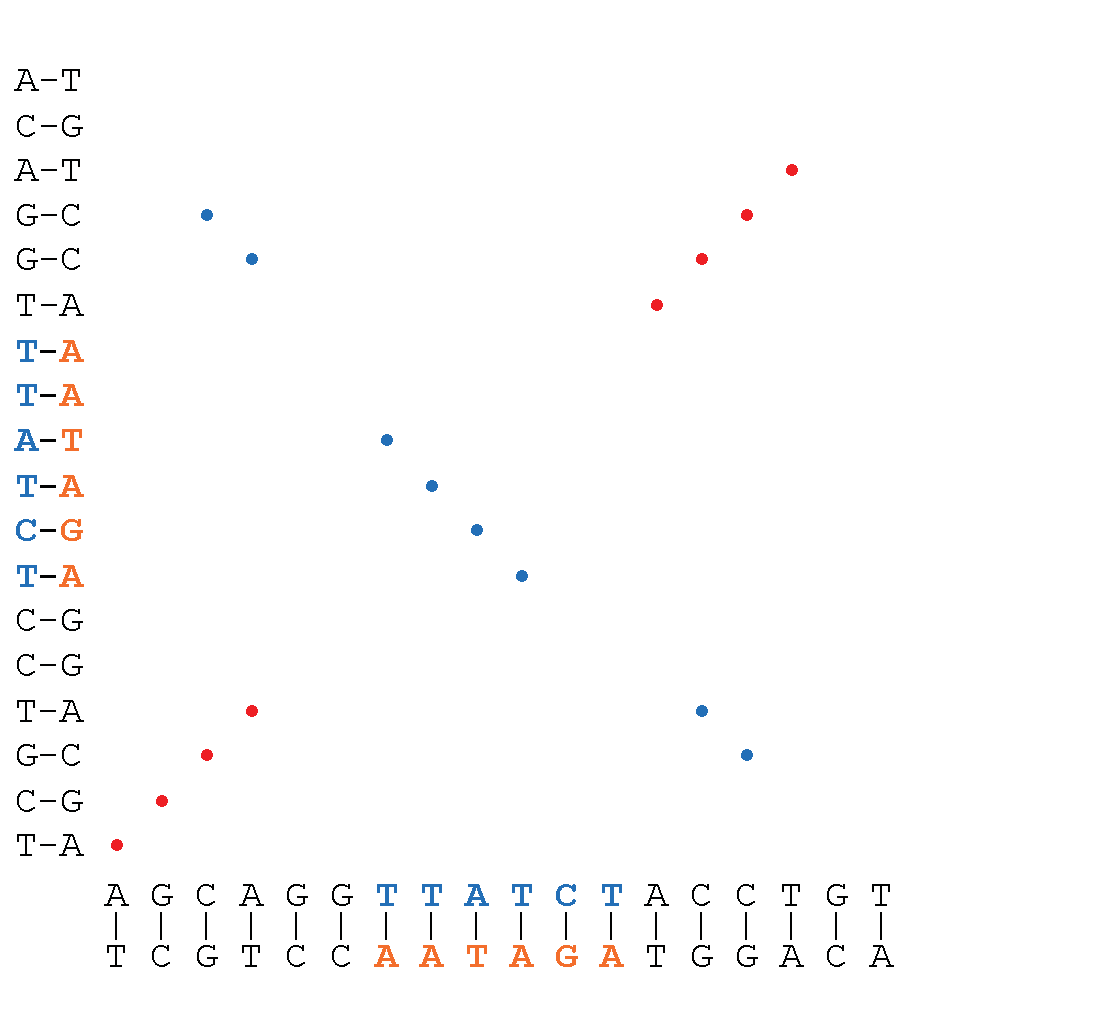
\includegraphics[width = 0.4\textwidth]{images/rearrangements/genomic_dot_plots-4}
\end{tabular}
\caption{A visualization of repeated $k$-mers within the string \textnucl{AGCAGGTTATCTCCCTGT} for $k=3$ (top left) and $k=2$ (top right). (Bottom left) We add blue points to the plot shown in in the upper left corner to indicate reverse complementary $k$-mers.  For example, \textnucl{CCT} and \textnucl{AGG} are reverse complementary 3-mers in \textnucl{AGCAGGTTATCTTCCTGT}. (Bottom right): Genomic dot-plot showing shared 3-mers between \textnucl{\black{AGCAGG}\Blue{TTATCT}\black{CCCTGT}} and \textnucl{\black{AGCAGG}\Orange{AGATAA}\black{CCCTGT}}.  The latter sequence resulted from the former sequence by a reversal of the segment \textnucl{\Blue{TTATCT}}. Each point $(x, y)$ corresponds to a $k$-mer shared by the two genomes.  Red points indicate identical shared $k$-mers, whereas blue points indicate reverse complementary $k$-mers. Note that the dot-plot has four ``noisy'' blue points in the diagram: two in the upper left corner, and two in the bottom right corner. You will also notice that red dots can be connected into line segments with slope 1 and blue dots can be connected into line segments with slope -1. The resulting three synteny blocks (\textnucl{\Red{AGCAGG}}, \textnucl{\Blue{TTATCT}}, and \textnucl{\Red{CCCTGT}}) correspond to three diagonals (each formed by four points) in the dot-plot.}
\label{fig:genomic_dot_plots}
\end{figure}

\begin{center}
\mySfFamily
\tabcolsep = 1em
\begin{tabular}{l l l l}
\textnucl{\phantom{xxxx}}0 & 0 \textnucl{\phantom{xxxx}} & \textnucl{\phantom{xxxx}4} & \textnucl{\phantom{xxxxxx}}6\\[-0.25ex]
\textnucl{\phantom{xxxx}\Red{AAA}CTCATC} & \textnucl{\Blue{AAA}CTCATC} & \textnucl{AAAC\Red{TCA}TC\phantom{xx}} & \textnucl{AAACTC\Red{ATC}}\\
\textnucl{TTTC\Red{AAA}TC\phantom{xxxx}} & \textnucl{\Blue{TTT}CAAATC} & \textnucl{\phantom{xx}TT\Red{TCA}AATC} & \textnucl{TTTCAA\Red{ATC}}\\
\textnucl{\phantom{xxxx}}4 & 0 & \textnucl{\phantom{xxxx}}2 & \textnucl{\phantom{xxxxxx}}6
\end{tabular}
\end{center}

\noindent We can further generalize the genomic dot plot to analyze the shared $k$-mer content of two genomes.  We color the point $(x,y)$ red if the two genomes share a $k$-mer at respective positions $x$ and $y$; we color $(x, y)$ blue if the two genomes have reverse complementary $k$-mers at these starting positions.  See \autoref{fig:genomic_dot_plots} (bottom right).\\

\begin{exercise}[
Find all shared 2-mers of \textnucl{AAACTCATC} and \textnucl{TTTCAAATC}.
]\end{exercise}

\begin{problem}[Shared \textit{k}-mers Problem]{Given two strings, find all their shared \textit{k}-mers.}{An integer $k$ and two strings.}{All $k$-mers shared by these strings, in the form of ordered pairs $(x, y)$.}
\protect\computationalproblem[Shared \textit{k}-mers Problem]{-4.89}
\end{problem}

\noindent Since downloading long human and mouse chromosomes is time-consuming, we will instead solve the Shared $k$-mers Problem for the bacteria \textit{E. coli} and \textit{S. enterica}, which we have already encountered in previous chapters.\\

\begin{exercise}[Answer the following questions regarding counting shared $k$-mers.
\begin{enumerate}
\vspace{-1ex}
\item Compute the expected number of 30-mers shared by two random strings, each a billion nucleotides long.
\vspace{-1ex}
\item How many shared 30-mers do the \textit{E. coli} and \textit{S. enterica} genomes have?
\end{enumerate}
\vspace{-1ex}
]\end{exercise}

\noindent In previous chapters, we have worked with the genomes for the bacteria \textit{E. coli} and \textit{S. enterica}, each of which is about 5 million nucleotides long.  It can be shown that the expected number of shared 30-mers between two random 5 million nucleotide-long sequences is approximately $\left. 2 \cdot (5 \cdot 10^6)^2 \middle/ 4^{30}\right. \approx 1/20,000$.

Yet solving the Shared $k$-mers Problem for \textit{E. coli} and \textit{S. enterica} yields over 200,000 pairs $(x,y)$ corresponding to shared 30-mers. The surprisingly large number of shared 30-mers indicates that \textit{E. coli} and \textit{S. enterica} are close relatives that have retained many similar genes inherited from their common ancestor. However, these genes may be arranged in a different order in the two species: how can we infer synteny blocks from these genomes' shared $k$-mers? The genomic dot-plot plot for \textit{E. coli} and \textit{S. enterica} is shown in \autoref{fig:e-coli_dot-plot}.\par

\begin{figure}[h]
\mySfFamily
\centering
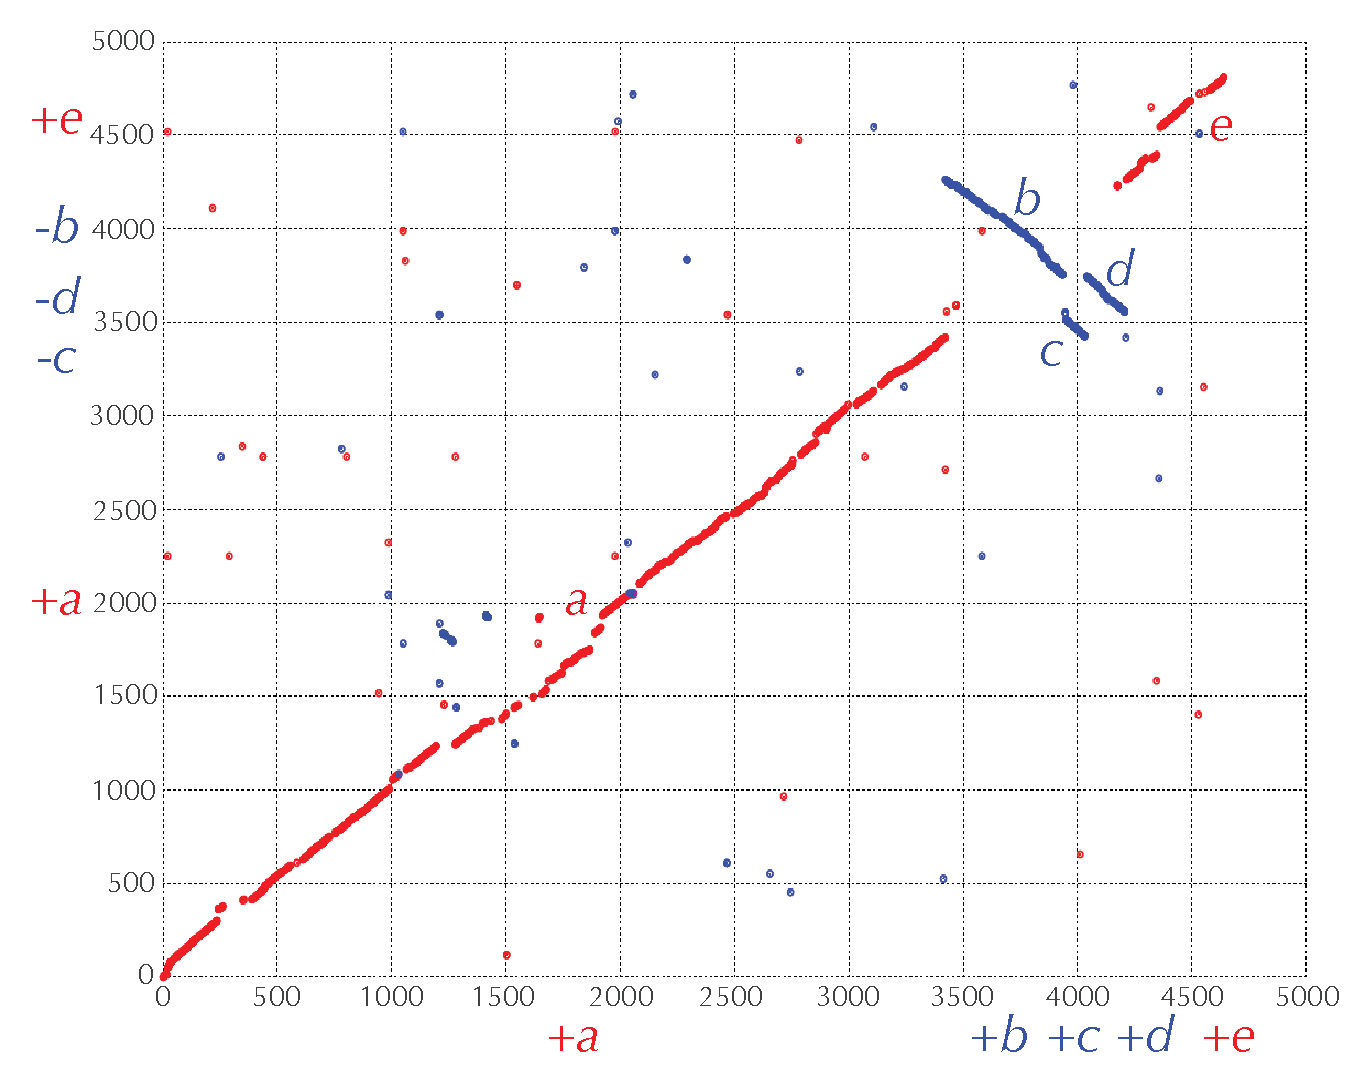
\includegraphics[width = 0.856\textwidth]{images/rearrangements/e-coli_dot-plot}
\caption{Genomic dot-plot of \textit{E. coli} (horizontal axis) and \textit{S. enterica} (vertical axis) for $k = 30$. Each point $(x, y)$ corresponds to a $k$-mer shared by the two genomes.  Red points indicate identical shared $k$-mers, whereas blue points indicate reverse complementary $k$-mers.  Each axis is measured in kilobases (thousands of base pairs).}
\label{fig:e-coli_dot-plot}
\end{figure}

\begin{qbox}[
Can you see the synteny blocks in the genomic dot-plot in \autoref{fig:e-coli_dot-plot}?
]\end{qbox}

\phantomsection
\subsection{From shared \emph{k}-mers to synteny blocks}
\label{subsec:from_shared_k-mers_to_synteny_blocks}

The genomic dot-plot in \autoref{fig:e-coli_dot-plot} indicates five regions of similarity in the form of points that clump together into approximately diagonal segments.  These segments are labeled by \red{\textit{a}}, \blue{\textit{b}}, \blue{\textit{c}}, \blue{\textit{d}}, and \red{\textit{e}} according to the order in which they appear in the \textit{E. coli} genome; we ignore smaller diagonals such as the short blue diagonal starting around position 1.3 million in \textit{E. coli} and around position 1.9 million in \textit{S. enterica}. For example, while \red{\textit{a}} corresponds to a long diagonal segment of slope 1 that covers approximately the first 3.5 million positions in both genomes, \blue{\textit{b}} corresponds to a shorter diagonal segment of slope -1 that starts shortly before position 3.5 million in \textit{E. coli} and shortly after position 4 million in \textit{S. enterica}. Although \blue{\textit{b}} appears small in \autoref{fig:e-coli_dot-plot}, don't be fooled by the scale of the figure; \blue{\textit{b}} is over 100,000 nucleotides long and contains nearly 100 genes.

The segments \red{\textit{a}}, \blue{\textit{b}}, \blue{\textit{c}}, \blue{\textit{d}}, and \red{\textit{e}} give us the synteny blocks that we have been looking for. If we project these blocks onto the $x$- and $y$-axes, then the ordering of blocks on each axis corresponds to the ordering of synteny blocks in the respective bacterium.  The ordering of synteny blocks in \textit{E. coli} (plotted on the $x$-axis) is $(\red{+a}$ $\blue{+b}$ $\blue{+c}$ $\blue{+d}$ $\red{+e})$, and the ordering in \textit{S. enterica} (y-axis) is $(\red{+a}$ $\blue{-c}$ $\blue{-d}$ $\blue{-b}$ $\red{+e})$.  Note that the blue letters in \textit{S. enterica} are assigned a negative sign because these blocks were constructed from reverse complementary $k$-mers. \autoref{fig:e-coli_dot-plot} also illustrates what the directions of blocks are --- they respectively correspond to diagonals in the dot-plot with slope 1 (blocks with a ``+'' sign) and  slope -1 (blocks with a ``-'' sign).

We have therefore represented two bacterial genomes using just five synteny blocks.  Of course, this simplification required us to throw out some noisy points in the genome plot, corresponding to tiny regions of similarity that did not surpass a threshold length in order to be considered synteny blocks.

We are now ready to construct the 11 human-mouse synteny blocks originally presented in \autoref{fig:mouse_and_human_synteny_blocks} (page \pageref{fig:mouse_and_human_synteny_blocks}), but since the human and mouse X chromosomes are rather long, we will instead provide you with all positions $(x,y)$ where they share significant similarities. \autoref{fig:synteny_blocks} (top left) presents the resulting genomic dot-plot for the human and mouse X chromosomes, where each dot represents a long similar region rather than a shared $k$-mer. Our eyes immediately find 11 diagonals in this plot corresponding to the human-mouse X chromosome synteny blocks --- problem solved! We state this problem as the Finding Synteny Blocks Problem.\\

\begin{figure}[p]
\mySfFamily
\centering
\begin{tabular}{c @{\hskip 2em} c}
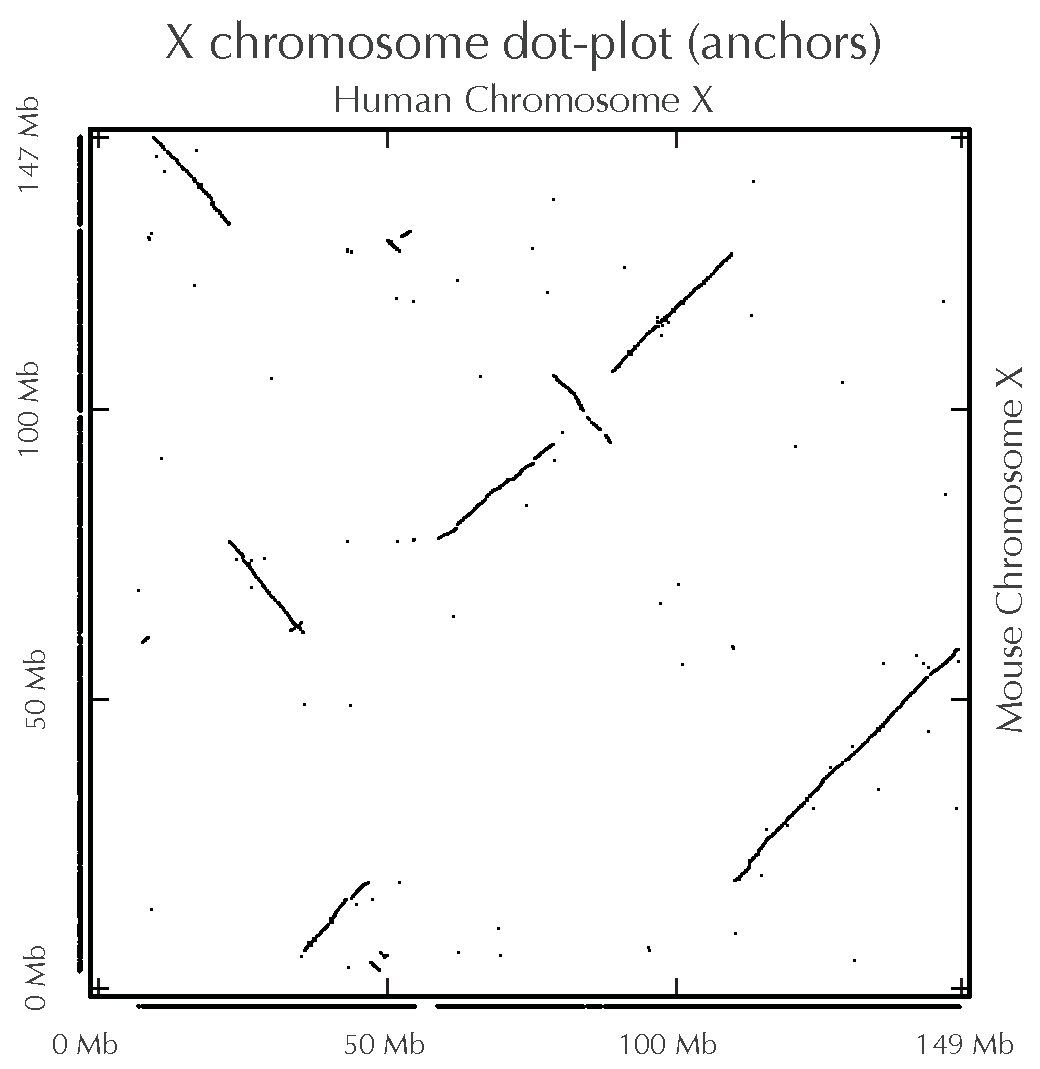
\includegraphics[width = 0.43\textwidth]{images/rearrangements/synteny_blocks-1} & 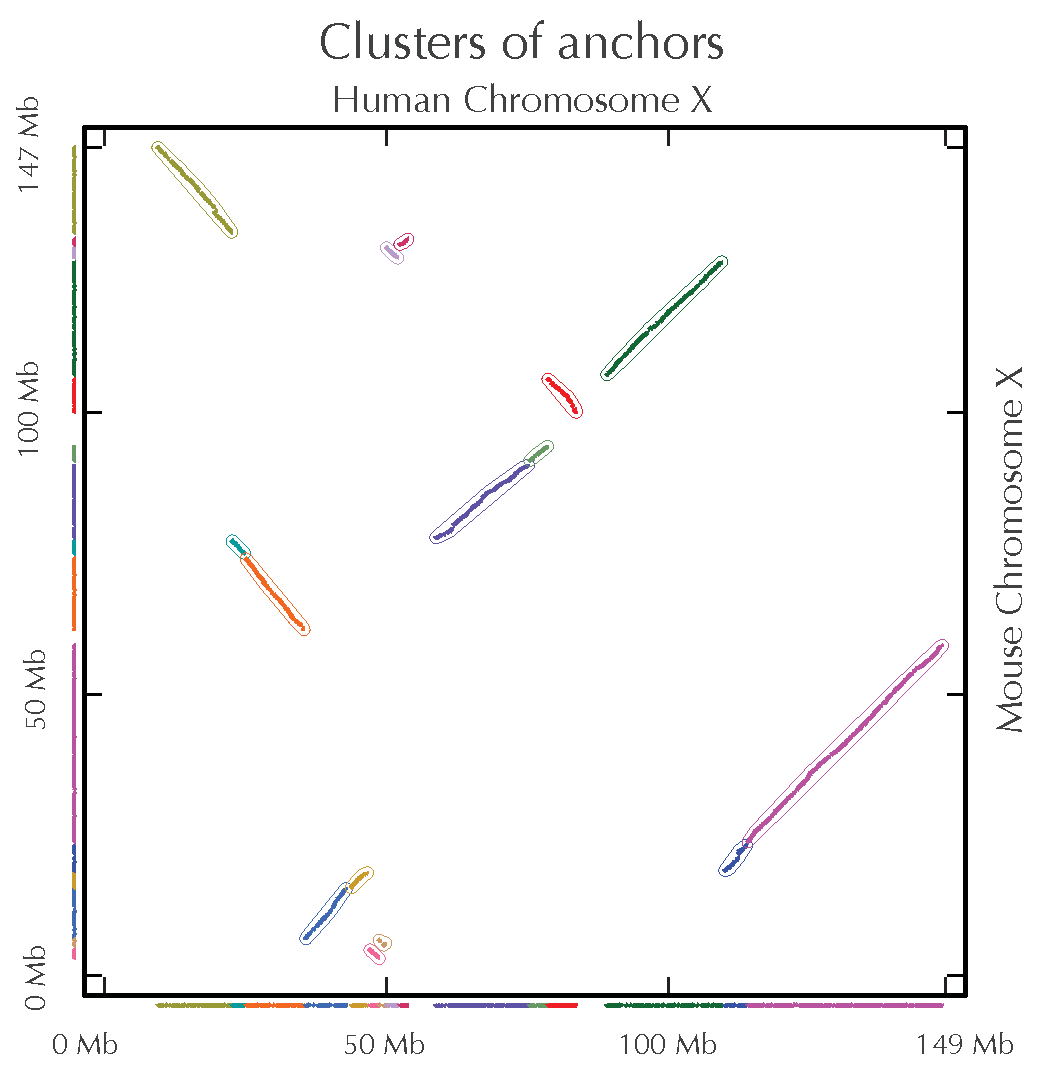
\includegraphics[width = 0.43\textwidth]{images/rearrangements/synteny_blocks-2}\\[3ex]
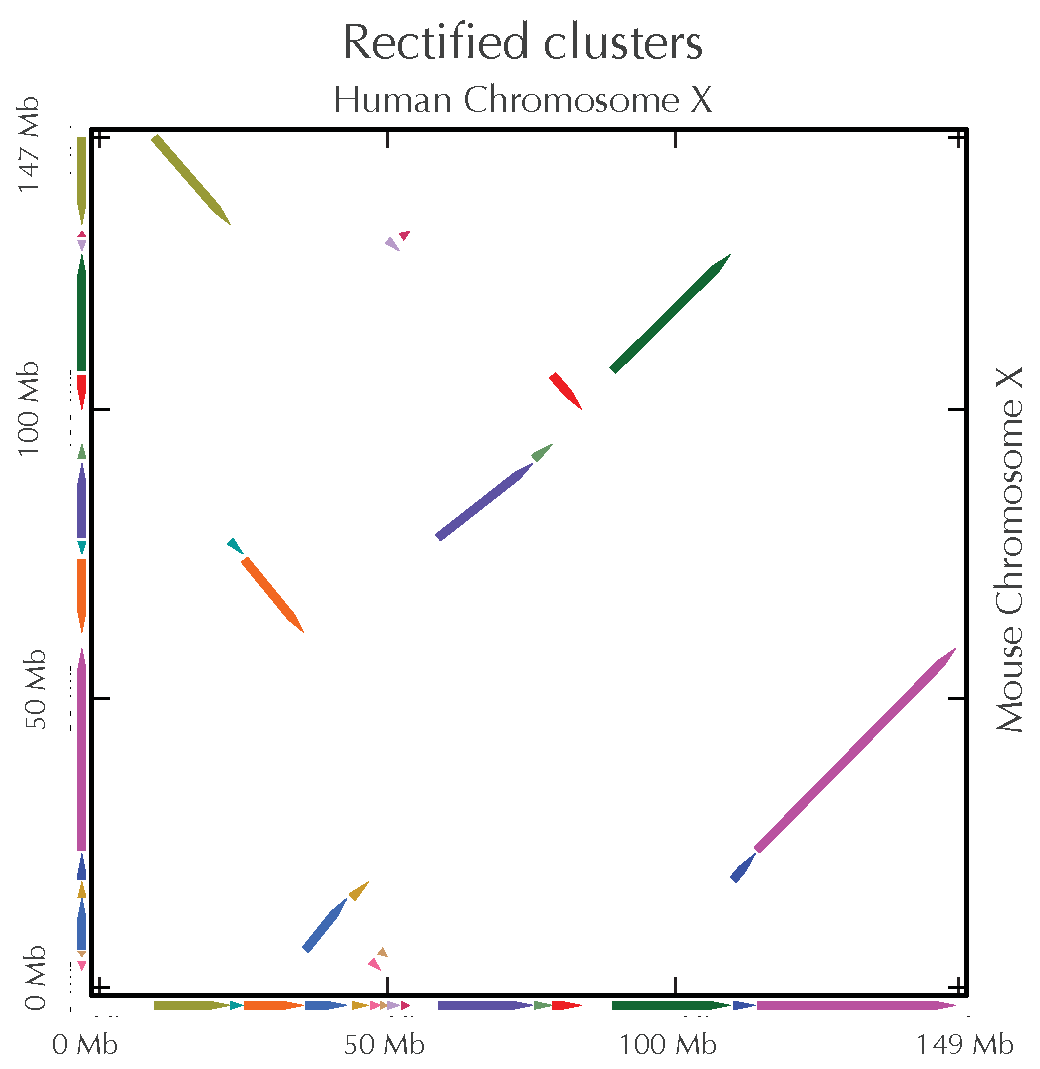
\includegraphics[width = 0.43\textwidth]{images/rearrangements/synteny_blocks-3} & 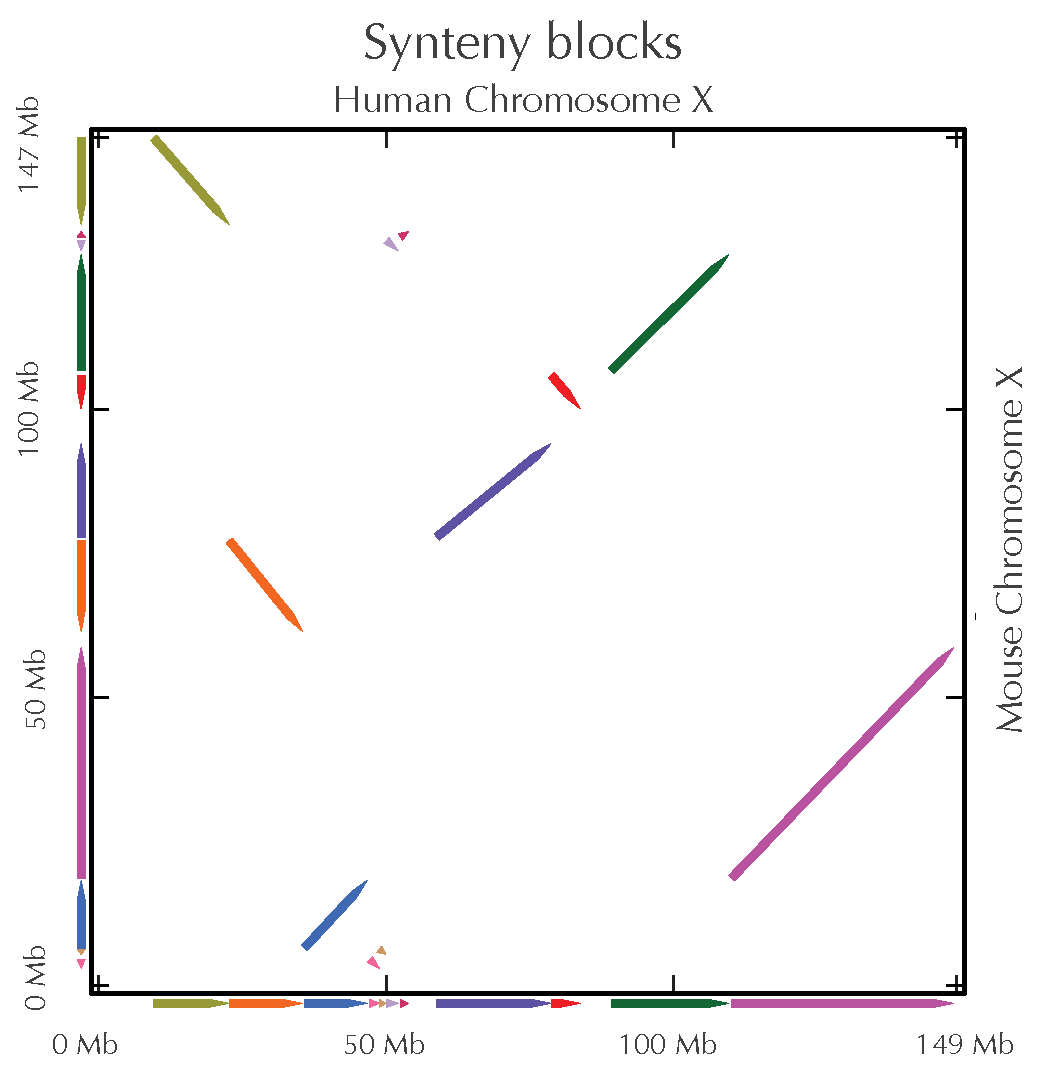
\includegraphics[width = 0.43\textwidth]{images/rearrangements/synteny_blocks-4}\\[3ex]
\end{tabular}
\caption{From local similarities to synteny blocks. (Top left) The genomic dot-plot for the human and mouse X chromosomes, representing all positions $(x,y)$ where they share significant similarities.  In contrast with \autoref{fig:e-coli_dot-plot}, we do not distinguish between red and blue dots. (Top right) Clusters (connected components) of points in the genomic dot-plot are formed by constructing the synteny graph.  (Bottom left) Rectified clusters from the synteny graph transform each cluster into an exact diagonal of slope $\pm 1$. (Bottom right) Aggregated synteny blocks.  Projection of the synteny blocks to the $x$-and $y$-axes results in the arrangements of synteny blocks in the respective human and mouse genomes $(+1$ $+2$ $+3$ $+4$ $+5$ $+6$ $+7$ $+8$ $+9$ $+10$ $+11)$ and  $(+1$ $-7$ $+6$  $-10$  $+9$  $-8$  $+2$ $-11$ $-3$ $+5$ $+4)$.}
\label{fig:synteny_blocks}
\end{figure}

\begin{problem}[Finding Synteny Blocks Problem]{Find diagonals in the genomic dot-plot.}{A set of points \textvar{DotPlot} in the plane.}{A set of diagonals in \textvar{DotPlot} representing synteny blocks.}
\end{problem}

\noindent Unfortunately, it remains unclear how to write a program to do what our eyes found to be so easy; we hope you have already noticed that the Finding Synteny Blocks Problem is not a well-formulated computational problem. As we have mentioned, the diagonals in \autoref{fig:synteny_blocks} (top left) are not perfect. Moreover, there are many gaps within diagonals that cannot be seen by the human eye but will become apparent if we zoom into the genome plot. It is thus absolutely unclear what method the human brain is using to transform the dots into the 11 diagonals in the genomic dot-plot.\\

\begin{qbox}[
How can we translate the brain's tendency to construct the diagonals that you see in \autoref{fig:synteny_blocks} (top left) into an algorithm that a computer can understand?
]\end{qbox}

\vspace{-0.5\baselineskip}

\phantomsection
\subsection{Synteny blocks as connected components in graphs}
\label{subsec:synteny_blocks_as_connected_components_in_graphs}

The reason why you can easily see the synteny blocks in a genomic dot-plot is that your brain is good at \textdef{clustering} nearby points in an image.  To mimic this process with a computer, we therefore need a precise notion of clustering. Given a set of points \textvar{DotPlot} in the plane as well as a parameter \textit{maxDistance}, we will construct the (undirected) \textdef{synteny graph} $\textfunc{SyntenyGraph}(\textvar{DotPlot}, \textvar{maxDistance})$ by connecting two points in \textvar{DotPlot} with an edge if the distance between them does not exceed \textvar{maxDistance}.

Every graph can be divided into disjoint connected subgraphs called \textdef{connected components}.  The connected components in $\textfunc{SyntenyGraph}(\textvar{DotPlot}, \textvar{maxDistance})$ represent candidate synteny blocks between the two genomes (\autoref{fig:synteny_graph}).  When we construct the synteny graph for the human and mouse X chromosomes, we find a huge number of small connected components (the exact number depends on our choice of the \textvar{maxDistance} parameter). However, we will ignore these small connected components, since they may represent spurious similarities. We thus introduce a parameter called \textvar{minSize} representing the minimum number of points in a connected component that we will consider as forming a synteny block.  Our goal is to return all connected components having at least \textvar{minSize} nodes.\\

\begin{figure}[h]
\mySfFamily
\centering
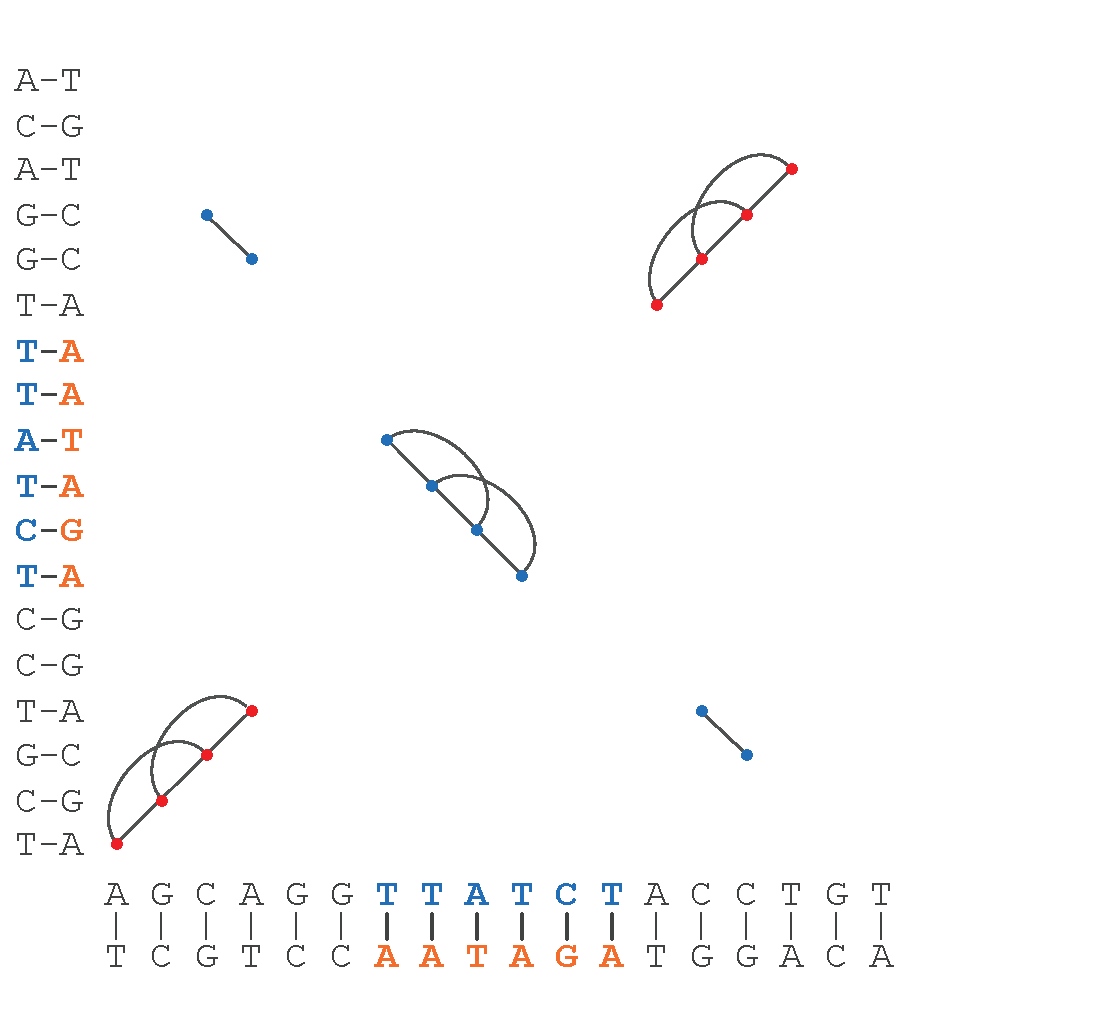
\includegraphics[width = 0.6\textwidth]{images/rearrangements/synteny_graph}
\caption{The graph $\textfunc{SyntenyGraph}(\textvar{DotPlot}, 4)$ constructed from the genomic dot-plot of \textnucl{\black{AGCAGG}\Blue{TTATCT}\black{CCCTGT}} and \textnucl{\black{AGCAGG}\Orange{AGATAA}\black{CCCTGT}}  for $k = 3$.  Note that the three synteny blocks (all of which have four nodes) correspond to diagonals in the genomic dot-plot.  We ignore the two smaller, noisy synteny blocks.}
\label{fig:synteny_graph}
\end{figure}

\begin{elaboration}
\begin{algorithmic}
\leftskip = \algindent %Needed to match the indentation of the text.
\Algorithm{SyntenyBlocks}{\textvar{DotPlot}, \textvar{maxDistance}, \textvar{minSize}}
	\State construct $\textfunc{SyntenyGraph}(\textvar{DotPlot}, \textvar{maxDistance})$
	\State find the connected components in $\textfunc{SyntenyGraph}(\textvar{DotPlot}, \textvar{maxDistance})$
	\State \output connected components of at least \textvar{minSize} nodes as candidate\\ \hspace{4.7em}synteny blocks
\EndAlgorithm
\end{algorithmic}
\end{elaboration}
%\protect\computationalproblem[e]{Find Synteny Blocks}{-27.5}

\fudgespace

\noindent As \autoref{fig:synteny_blocks} (top right) illustrates, \textalg{SyntenyBlocks} has a tendency to partition a single diagonal (as perceived by the human eye) into multiple diagonals due to gaps that exceed the parameter \textvar{maxDistance}. However, this partitioning is not a problem, since the broken diagonals can be combined later into a single (aggregated) synteny block. \par

\vspace{\baselineskip}

\begin{qbox}[
We have defined synteny blocks as large connected components in $\textfunc{SyntenyGraph}(\textvar{DotPlot}, \textvar{maxDistance})$ but have not described how to determine where these synteny blocks are located in the original genomes. Using \autoref{fig:synteny_blocks} as a hint, design an algorithm for finding this information.
]\end{qbox}

\noindent You should now be ready to solve the challenge problem and discover that the choice of parameters is one of the dark secrets of bioinformatics research.\\

\begin{finalchallenge}[Analyze Rearrangements Between X Chromosomes]{
Construct the synteny blocks for the human and mouse X chromosomes and compute the 2-break distance between the circularized human and mouse X chromosomes using the synteny blocks that you constructed. How does this distance change depending on the parameters \textvar{maxDistance} and \textvar{minSize}?
}\end{finalchallenge}

\phantomsection
\FloatBarrier
\section{Open Problem: Can Rearrangements Shed Light on Bacterial Evolution?}
\label{sec:rearrangements_open_problem}

Although there exist efficient algorithms for analyzing \emph{pairwise} genome rearrangements, constructing rearrangement scenarios for \emph{multiple} genomes remains an open problem. For example, we now know how to find a most parsimonious rearrangement scenario transforming the mouse X chromosome into the human X chromosome. However, the problem of finding a most parsimonious rearrangement scenario for the human, mouse and rat X chromosomes (let alone for their entire genomes) is a more difficult problem. The difficulties further amplify when we attempt to reconstruct a rearrangement history for dozens of mammalian genomes. To address this challenge, we start from the simpler (but still unsolved) case of bacterial genomes.

Let \textvar{Tree} be a tree (i.e., a connected acyclic undirected graph) with nodes labeled by some genomes. In the case of bacterial genomes, we assume that every node (genome) is labeled by a circular permutation on $n$ elements. Given an edge $e$ connecting nodes $v$ and $w$ in \textvar{Tree}, we define $\textfunc{Distance}(v, w)$ as the 2-break distance between genomes $v$ and $w$.  The \textdef{tree distance} $\textfunc{Distance}(\textvar{Tree})$ is the sum 

\begin{center}
$\sum\limits_{\text{all edges }(v, w)\text{ in \textvar{Tree}}}{\textfunc{Distance}(v, w)}$.
\end{center}

Given a set of genomes $P_1, \ldots ,P_n$ and an evolutionary tree \textvar{Tree} with $n$ leaves labeled by $P_1, \ldots ,P_n$, the Ancestral Genome Reconstruction Problem attempts to reconstruct  genomes at the internal nodes of the tree such that $\textfunc{Distance}(\textvar{Tree})$ is minimized across all possible reconstructions of genomes at internal nodes.\\

\begin{problem}[Ancestral Genome Reconstruction Problem]{Given a tree with leaves labeled by genomes, reconstruct ancestral genomes that minimize the tree distance.}{A tree \textvar{Tree} with each leaf labeled by a genome.}{Genomes \textvar{AncestralGenomes} assigned to the internal nodes of \textvar{Tree} such that $\textfunc{Distance}(\textvar{Tree})$ is minimized across all possible choices of \textvar{AncestralGenomes}.}
\end{problem}

\noindent In the case when \textvar{Tree} is not given, we need to infer it from the genomes.\\

\begin{problem}[Multiple Genome Rearrangement Problem]{Given a set of genomes, reconstruct a tree with leaves labeled by these genomes and minimum tree distance.}{A set of genomes.}{A tree \textvar{Tree} with leaves labeled by these genomes and internal nodes labeled by (unknown) genomes \textvar{AncestralGenomes} such that $\textfunc{Distance}(\textvar{Tree})$ is minimal among all possible choices of \textvar{Tree} and \textvar{AncestralGenomes}.}
\end{problem}

\noindent While many algorithms have been proposed for the Multiple Genome Rearrangement Problem, they have mainly been applied to analyze mammalian evolution (see \cite{ma_2008} and \cite{alekseyev_pevzner_2009} for some examples).  However, there have been hardly any applications of the Multiple Genome Rearrangement Problem for analyzing bacterial evolution. The fact that bacterial genomes are approximately 1000 times smaller than mammalian genomes does not make this problem 1000 times easier. In fact, there are unique challenges and opportunities in bacterial evolutionary research.

Consider 100 genomes from three closely related bacterial genera, \textit{Salmonella}, \textit{Shigella}, and \textit{Escherichia}, whose various species are responsible for dysentery, typhoid fever, and a variety of foodborne illnesses.  After you construct synteny blocks shared by all these genomes, you will see that there are relatively few (usually fewer than 10) rearrangements between every pair of genomes. However, solving the Multiple Genome Rearrangement Problem even in the case of closely related genomes presents a formidable challenge, and nobody has been able to construct a rearrangement scenario for more than a couple dozen --- let alone 100! --- species yet.

After you solve this puzzle, you will be able to address the question of whether there are fragile regions in bacterial genomes. Answering this question for a pair of bacterial genomes, like we did for the human and mouse genomes, may not be possible because there are typically fewer than 10 rearrangements between them. But answering this question for 100 bacterial genomes may be possible if we witness the same breakage occurring independently on many branches of the evolutionary tree. However, you will need to develop algorithms to analyze fragile regions in multiple (rather than pairwise) genomes.

After you construct the evolutionary tree, you will also be in a position to analyze the question of what triggers rearrangements. While many authors have discussed the causes of fragility, this question remains open, with no shortage of hypotheses. \cite{zhao_bourque_2009} demonstrated that many rearrangements are flanked by \textdef{matching duplications}, a pair of long similar regions located within a pair of breakpoint regions corresponding to a rearrangement event. However, they limited their study to mammalian evolution, and it remains unclear what triggers rearrangements in bacteria; can you answer this question?\\

\phantomsection
\FloatBarrier
\section{Detours}
\label{sec:detours_rearrangements}

\phantomsection
\begin{detour}[Why is the gene content of mammalian X chromosomes so conserved?]{why_is_the_gene_content_of_mammalian_x_chromosomes_so_conserved}

While mammalian X chromosomes are enriched in genes related to sexual reproduction, most of the approximately 1000 genes on the X chromosome have nothing to do with gender. Ideally, they should be expressed (i.e., transcribed and eventually translated) in roughly the same quantities in females and males.  But since females have two X chromosomes and males have only one, it would seem that all the genes on the X chromosome should have twice the expression level in females.  This imbalance would lead to a problem in the complex cellular system of checks and balances underlying gene expression.

The need to balance gene expression in males and females led to the evolution of special mechanisms of \textdef{dosage compensation}, or the inactivation of one X chromosome in females to equalize gene expression between the sexes. Because of dosage compensation, the gene content of the X chromosome is highly conserved between mammalian species because if a gene jumps off the X chromosome, then its expression may double, thus creating a genetic imbalance.
\end{detour}

\phantomsection
\begin{detour}[Discovery of genome rearrangements]{discovery_of_genome_rearrangements}
\textdef{Genetic maps}, which show the positions of genes along chromosomes, were used by Thomas Hunt Morgan's lab at Columbia as early as 1913.  An amazing thing happened in 1921 when Morgan's student Alfred Sturtevant created genetic maps for two different species of \textit{Drosophila}. It was clear just by looking at the maps that an entire genomic interval had been inverted in one species as compared to another! The only reasonable explanation was that a reversal had flipped this chromosomal interval around. Sturtevant posited that this had happened when the chromosome became tangled on itself and formed a loop.

Another breakthrough occurred with the discovery that the salivary glands of \textit{Drosophila} contain \textdef{polytene cells}.  In normal cellular division, each daughter cell receives one copy of the genome.  However, in the nuclei of polytene cells, DNA replication occurs repeatedly in the absence of cell division.  The resulting chromosomes then knit themselves together into much larger ``superchromosomes'' called \textdef{polytene chromosomes}.

Polytene chromosomes serve a practical purpose for the fruit fly, which uses the extra DNA to boost the production of gene transcripts, producing lots of sticky saliva. But the human value of polytene chromosomes is perhaps greater.  When Sturtevant and his collaborator, Theodosius Dobzhansky, looked at polytene chromosomes under a microscope, they were able to witness the work of rearrangements  firsthand in tangled mutant chromosomes. In 1938, Sturtevant and Dobzhansky published a milestone paper with an evolutionary tree presenting a rearrangement scenario with 17 reversals for various species of \textit{Drosophila}. Their drawing was the first evolutionary tree in history to be constructed based on molecular data.

%\begin{figure}[h]
%\mySfFamily
%\centering
%\textbf{THIS FIGURE IS DEFINITELY COPYRIGHTED}
%\caption{Evolutionary tree of various \textit{Drosophila} species based on their gene arrangements. Two species connected by an edge in the tree differ by a single reversal.}
%\label{fig:drosophila_phylogeny}
%\end{figure}
\end{detour}

\phantomsection
\begin{detour}[The exponential distribution]{the_exponential_distribution}
A \textdef{Bernoulli trial} is a random experiment with two possible outcomes, ``success'' (having probability $p$) and ``failure'' (having probability $1-p$). The \textdef{geometric distribution} is the probability distribution underlying the random variable $X$ representing the number of Bernoulli trials needed to obtain the first success:

\begin{center}
$\mathrm{Pr}(X = k) = (1-p)^{k-1}p$.
\end{center}

A \textdef{Poisson process} is a continuous-time stochastic process counting the number of events in a given time interval, if we assume that the events occur independently at a constant rate. For example, the Poisson process offers a good model of time points for passengers arriving to a large train station.  If we assume that the number of passengers arriving during a very small time interval $\epsilon$ is $\lambda \cdot \epsilon$ (where $\lambda$ is a constant), then we are interested in the probability $F(X)$ that nobody will arrive to the station during a time interval $X$. The \textdef{exponential distribution} describes the time between events in a Poisson process.\\

\begin{qbox}[
Do you see any similarities between the Poisson process and the Bernoulli trials or between the exponential and geometric distributions? 
]\end{qbox}

\noindent The exponential distribution is merely the continuous analogue of the geometric distribution. More precisely, the Poisson process is characterized by a \textdef{rate parameter} $\lambda$, such that the number of events $k$ in the time interval $[X, X+\epsilon]$ follows the \textdef{Poisson probability distribution}:

\begin{center}
$\left. e^{-\lambda \cdot \epsilon}(\lambda \cdot \epsilon)^k \middle/ k!\right.$
\end{center}

\noindent The \textdef{probability density function} of the exponential distribution is  $\lambda e^{-\lambda \cdot X}$ (compare with the geometric distribution shown in \autoref{fig:probability_density_functions}).\\

\begin{figure}[h]
\centering
\begin{tabular}{c @{\hskip3em} c}
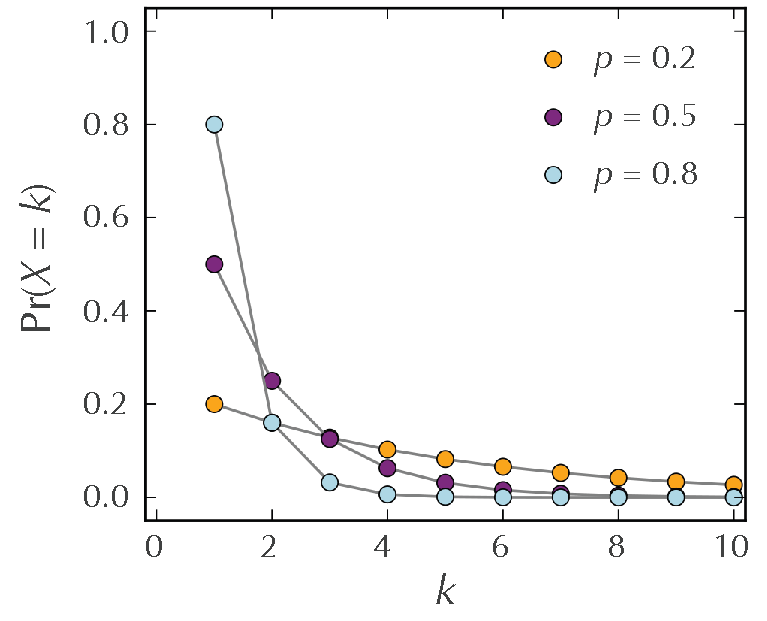
\includegraphics[width = 0.4\textwidth, valign = b]{images/rearrangements/geometric_distribution} & 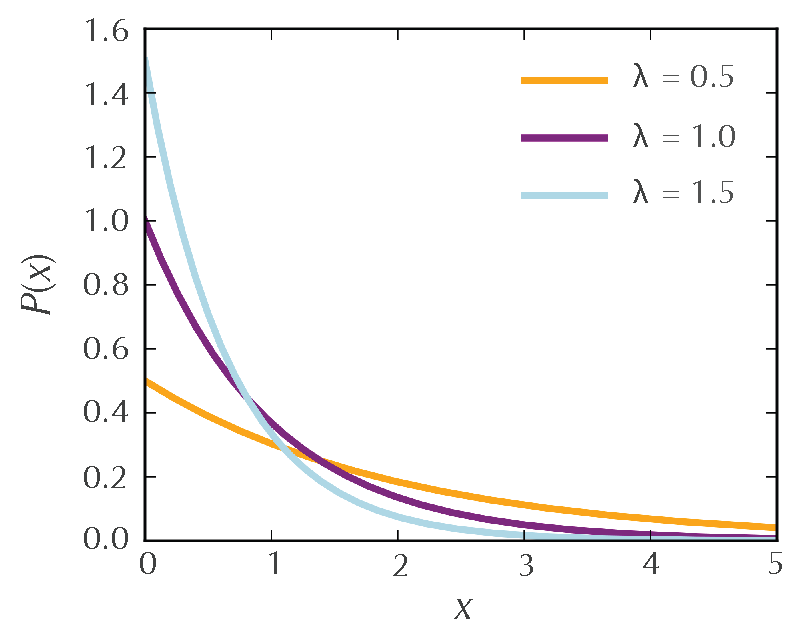
\includegraphics[width = 0.42\textwidth, valign = b]{images/rearrangements/exponential_distribution}\\
\end{tabular}
\caption{The probability density functions of the geometric (left) and exponential (right) distributions, each provided for three different parameter values.  Courtesy Skbkekas (Wikipedia user).}
\label{fig:probability_density_functions}
\end{figure}

\end{detour}

%\phantomsection
%\begin{detour}[Occam's Razor]{occams_razor}
%William of Ockham was an influential philosopher in the 14th Century. The principle of Occam's razor states that one should proceed to simpler theories until simplicity can be traded for greater explanatory power. Though the principle is attributed to Occam, Ptolemy (c. AD 90 -- c. AD 168) stated, ``We consider it a good principle to explain the phenomena by the simplest hypothesis possible.''  Thomas Aquinas (1225-1274) added that ``it is superfluous to suppose that what can be accounted for by a few principles has been produced by many''.  After Occam, Isaac Newton (1642-1727) stated, ``We are to admit no more causes of natural things than such as are both true and sufficient to explain their appearances.'' Francis Crick, on the other hand, commented on limitations of Occam's razor in biology: ``While Occam's razor is a useful tool in the physical sciences, it can be a very dangerous implement in biology. It is thus very rash to use simplicity and elegance as a guide in biological research.''
%\end{detour}

\vspace{-0.5\baselineskip}

\phantomsection
\begin{detour}[Bill Gates and David X. Cohen flip pancakes]{bill_gates_and_david_x_cohen_flip_pancakes}
Before biologists faced genome rearrangement problems, mathematicians posed the \textdef{Pancake Flipping Problem}, arising from the following hypothetical waiter's conundrum.

\begin{quote}
\textit{The chef in our place is sloppy, and when he prepares a stack of pancakes they come out all different sizes. Therefore, when I deliver them to a customer, on the way to a table I rearrange them (so that the smallest winds up on top, and so on, down to the largest at the bottom) by grabbing several from the top and flipping them over, repeating this (varying the number I flip) as many times as necessary. If there are $n$ pancakes, what is the maximum number of flips that I will ever have to use to rearrange them?}
\end{quote}

Formally, a \textdef{prefix reversal} is a reversal that flips a prefix, or initial interval, of a permutation. The \textdef{Pancake Flipping Problem} corresponds to sorting unsigned permutations by prefix reversals.  For example, the series of prefix reversals shown below ignores signs and represents the sorting of an \textdef{unsigned permutation}, $(1 ~ 7 ~ 6 ~ 10 ~ 9 ~ 8 ~ 2 ~ 11 ~ 3 ~ 5 ~ 4)$, into the \textdef{identity unsigned permutation}, $(1 ~ 2 ~ 3 ~ 4 ~ 5 ~ 6 ~ 7 ~ 8 ~ 9 ~ 10 ~ 11)$.  The inverted interval is shown in red, and sorted intervals at the end of the permutation are shown in blue.

\begin{center}
\mySfFamily
\tabcolsep = 0.5em
\begin{tabular}{r @{\hskip0em} c c c c c c c c c c c @{\hskip0em} l}
$($ & \Red{1} & \Red{7} & \Red{6} & \Red{10} & \Red{9} & \Red{8} & \Red{2} & \Red{11} & 3 & 5 & 4 & $)$\\[-0.25ex]
$($ & \Red{11} & \Red{2} & \Red{8} & \Red{9} & \Red{10} & \Red{6} & \Red{7} & \Red{1} & \Red{3} & \Red{5} & \Red{4} & $)$\\[-0.25ex]
$($ & \Red{4} & \Red{5} & \Red{3} & \Red{1} & \Red{7} & \Red{6} & \Red{10} & 9 & 8 & 2 & \Blue{11} & $)$\\[-0.25ex]
$($ & \Red{10} & \Red{6} & \Red{7} & \Red{1} & \Red{3} & \Red{5} & \Red{4} & \Red{9} & \Red{8} & \Red{2} & \Blue{11}& $)$\\[-0.25ex]
$($ & \Red{2} & \Red{8} & \Red{9} & 4 & 5 & 3 & 1 & 7 & 6 & \Blue{10} & \Blue{11} & $)$\\[-0.25ex]
$($ & \Red{9} & \Red{8} & \Red{2} & \Red{4} & \Red{5} & \Red{3} & \Red{1} & \Red{7} & \Red{6} & \Blue{10} & \Blue{11}& $)$\\[-0.25ex]
$($ & \Red{6} & \Red{7} & 1 & 3 & 5 & 4 & 2 & \Blue{8} & \Blue{9} & \Blue{10} & \Blue{11} & $)$\\[-0.25ex]
$($ & \Red{7} & \Red{6} & \Red{1} & \Red{3} & \Red{5} & \Red{4} & \Red{2} & \Blue{8} & \Blue{9} & \Blue{10} & \Blue{11} & $)$\\[-0.25ex]
$($ & \Red{2} & \Red{4} & \Red{5} & 3 & 1 & \Blue{6} & \Blue{7} & \Blue{8} & \Blue{9} & \Blue{10} & \Blue{11} & $)$\\[-0.25ex]
$($ & \Red{5} & \Red{4} & \Red{2} & \Red{3} & \Red{1} & \Blue{6} & \Blue{7} & \Blue{8} & \Blue{9} & \Blue{10} & \Blue{11} & $)$\\[-0.25ex]
$($ & \Red{1} & \Red{3} & 2 & \Blue{4} & \Blue{5} & \Blue{6} & \Blue{7} & \Blue{8} & \Blue{9} & \Blue{10} & \Blue{11} & $)$\\[-0.25ex]
$($ & \Red{3} & \Red{1} & \Red{2} & \Blue{4} & \Blue{5} & \Blue{6} & \Blue{7} & \Blue{8} & \Blue{9} & \Blue{10} & \Blue{11} & $)$\\[-0.25ex]
$($ & \Red{2} & \Red{1} & \Blue{3} & \Blue{4} & \Blue{5} & \Blue{6} & \Blue{7} & \Blue{8} & \Blue{9} & \Blue{10} & \Blue{11} & $)$\\[-0.25ex]
$($ & \Blue{1} & \Blue{2} & \Blue{3} & \Blue{4} & \Blue{5} & \Blue{6} & \Blue{7} & \Blue{8} & \Blue{9} & \Blue{10} & \Blue{11} & $)$\\
\end{tabular}
\end{center}

When we instead desire a minimum series of prefix reversals sorting a \emph{signed} permutation, the problem is called the \textdef{Burnt Pancake Flipping Problem} (each pancake is ``burnt'' on one side, giving it two possible orientations).\\

\begin{qbox}[
Prove that every unsigned permutation of length $n$ can be sorted using at most  $2 \cdot (n-1)$ prefix reversals.  Prove that every signed permutation of length $n$ can be sorted using at most $3 \cdot (n-1) + 1$ prefix reversals. 
]\end{qbox}

\noindent Bill Gates, an undergraduate student at Harvard in the mid-1970s, and Christos Papadimitriou, a professor at Harvard in the mid-1970s, made the first attempt to solve the Pancake Flipping Problem and proved that any permutation of length $n$ can be sorted with at most $5/3 \cdot (n + 1)$ prefix reversals, a result that would not be improved for three decades. David X. Cohen worked on the Burnt Pancake Flipping Problem at Berkeley before he left computer science to become a writer for \textit{The Simpsons} and eventually producer of \textit{Futurama}. Along with Manuel Blum, he demonstrated that the Burnt Pancake Flipping Problem can be solved with at most $2 \cdot (n - 1)$ prefix reversals.

\end{detour}

\phantomsection
\begin{detour}[Similar problems with different fates]{similar_problems_with_different_fates}
In the main text, we defined the breakpoint graph for circular chromosomes, but this structure can easily be extended to linear chromosomes. \autoref{fig:permutation_breakpoint_graph} depicts the human and the mouse X chromosomes as alternating red-black and blue-black paths (1st and 2nd panels). These two paths are superimposed in the 3rd panel to form the breakpoint graph, which has 5 alternating red-blue cycles.\\

\begin{figure}[h]
\mySfFamily
\centering
\begin{tabular}{c}

\includegraphics[width = 0.856\textwidth]{images/rearrangements/permutation_breakpoint_graph_1}\\[3ex]
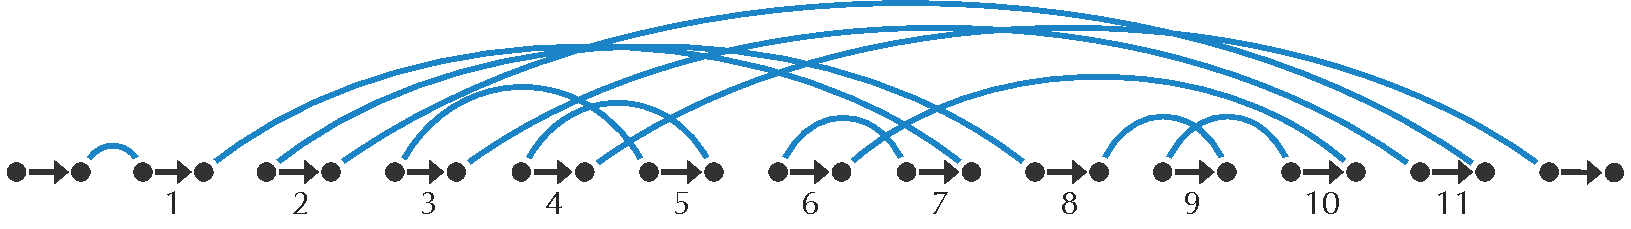
\includegraphics[width = 0.856\textwidth]{images/rearrangements/permutation_breakpoint_graph_2}\\[3ex]
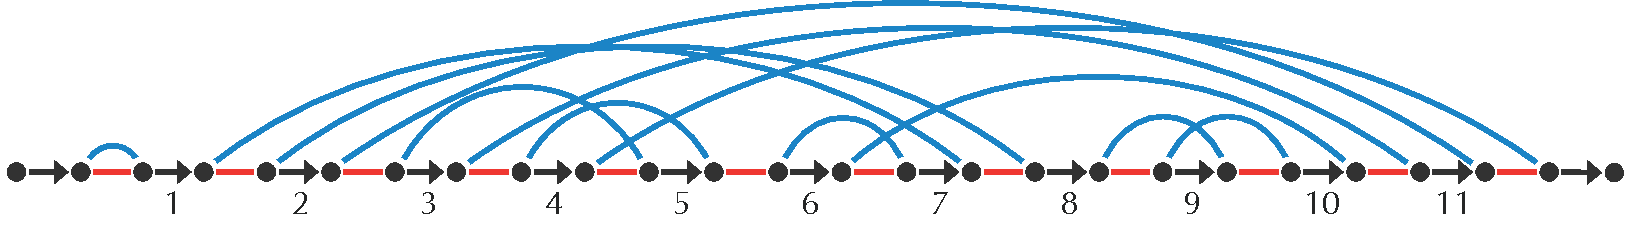
\includegraphics[width = 0.856\textwidth]{images/rearrangements/permutation_breakpoint_graph_3}\\[3ex]
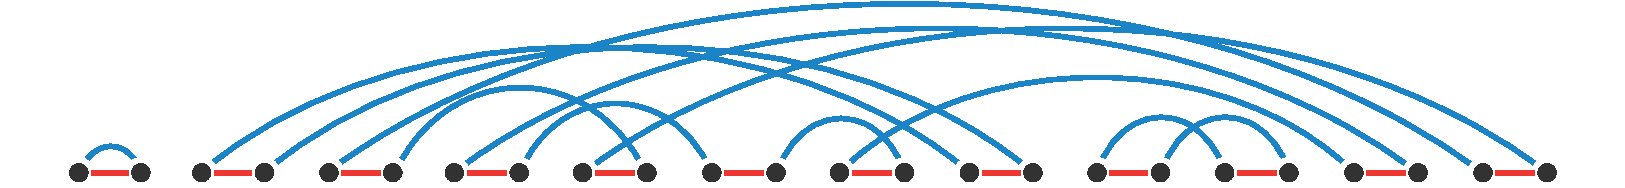
\includegraphics[width = 0.856\textwidth]{images/rearrangements/permutation_breakpoint_graph_4}
\end{tabular}
\caption{(1st panel) An alternating path of red and black edges representing the human X chromosome $(+1$ $+2$ $+3$ $+4$ $+5$ $+6$ $+7$ $+8$ $+9$ $+10$ $+11)$.   (2nd panel) An alternating path of blue and black edges representing the mouse X chromosome $(+1$ $-7$ $+6$ $-10$ $+9$ $-8$ $+2$ $-11$ $-3$ $+5$ $+4)$. (3rd panel) The breakpoint graph of the mouse and human X chromosomes is obtained by superimposing red-black and blue-black paths from the first two panels. (4th panel) To highlight the five alternating red-blue cycles in the breakpoint graph, black edges are removed.}
\label{fig:permutation_breakpoint_graph}
\end{figure}

\begin{qbox}[
Prove the following analogue of the Cycle Theorem for permutations: Given permutations $P$ and $Q$, any reversal applied to $P$ can increase $\textfunc{Cycles}(P, Q)$ by at most 1.
]\end{qbox}

\noindent While the number of trivial cycles is equal to $\textfunc{Blocks}(Q, Q)$  in the identity breakpoint graph of a circular permutation,  the trivial breakpoint graph of a linear permutation has $\textfunc{Blocks}(Q, Q) + 1$ trivial cycles.  Since the Cycle Theorem holds for linear permutations, perhaps the reversal distance $d_{\text{rev}}(P, Q)$ is equal to $\textfunc{Blocks}(P, Q) + 1 - \textfunc{Cycles}(P, Q)$ for linear chromosomes?  After all, for the human and mouse X chromosomes, $\textfunc{Blocks}(P, Q) + 1 - \textfunc{Cycles}(P, Q)$ is equal to $11 + 1 - 5 = 7$, which we already know to be the reversal distance between the human and mouse X chromosomes.\par

\vspace{\baselineskip}

\begin{qbox}[
Can you modify the proof of the 2-Break Distance Theorem to prove that  $d_{\text{rev}}(P, Q) = \textfunc{Blocks}(P, Q) + 1 - \textfunc{Cycles}(P, Q)$ for linear permutations $P$ and $Q$? 
]\end{qbox}

\noindent You can verify that the pesky permutation $P = (+2$ $+1)$ does not satisfy the condition $d_{\text{rev}}(P, I) = \textfunc{Blocks}(P, I) + 1 - \textfunc{Cycles}(P, I)$, where $I$ is the identity permutation, thus making it unlikely that we will be able to develop a simple algorithm for the computation of reversal distance. 

However, the lower bound $d_{\text{rev}}(P,Q) \geq \textfunc{Blocks}(P, Q) + 1 - \textfunc{Cycles}(P, Q)$  approximates the reversal distance between linear permutations extremely well. This intriguing performance raised the question of whether this bound is close to an exact formula. In 1999, Hannenhalli and Pevzner found this formula by defining two special types of breakpoint graph structures called ``hurdles'' and ``fortresses''. Denoting the number of hurdles and fortresses in $\textfunc{BreakpointGraph}(P, Q)$ by $\textfunc{Hurdles}(P, Q)$ and $\textfunc{Fortresses}(P, Q)$, respectively, they proved that the reversal distance $d_{\text{rev}}(P, Q)$  is given by

\begin{center}
$\textfunc{Blocks}(P, Q) + 1 - \textfunc{Cycles}(P, Q) + \textfunc{Hurdles}(P, Q) + \textfunc{Fortresses}(P, Q)$.
\end{center}

\noindent Using this formula, they developed a polynomial algorithm for computing $d_{\text{rev}}(P,Q)$.\\

\end{detour}

\phantomsection
\FloatBarrier
\section{Bibliography Notes}
\label{sec:rearrangements_bibliography_notes}

Alfred Sturtevant was the first to discover rearrangements while comparing gene orders in fruit flies (\cite{sturtevant_1921}). Together with Theodosius Dobzhansky, Sturtevant pioneered the analysis of genome rearrangements in molecular biology, publishing a milestone paper that presented a rearrangement scenario for many fruit fly species (\cite{sturtevant_dobzhansky_1936}).  The Random Breakage Model was proposed by \cite{ohno_1973}, further developed by \cite{nadeau_taylor_1984}, and refuted by \cite{pevzner_tesler_2003a}.

The notion of the breakpoint graph described in this chapter was proposed by \cite{bafna_pevzner_1996}. The polynomial algorithm for sorting by reversals was developed by \cite{hannenhalli_pevzner_1999}. The synteny block construction algorithm presented in this chapter was described by \cite{pevzner_tesler_2003b}. The 2-break operation was introduced in \cite{yancopoulos_2005} under the name of ``double cut and join''.

The first algorithmic analysis of the Pancake Flipping problem was described by \cite{gates_papadimitriou_1979}.  The first algorithmic analysis of the Burnt Pancake Flipping problem was described by \cite{cohen_blum_1995}.

The Multiple Genome Rearrangement problem was addressed by \cite{ma_2008} and \cite{alekseyev_pevzner_2009}. \cite{zhao_bourque_2009} observed that matching  duplications may trigger genome rearrangements.

\chapter{DCJ-Indel Sorting Revisited}

\section{Abstract}        % Do not use inserted blank lines (ie \\) until main body of text.
{\bf Background}: The introduction of the double cut and join operation (DCJ) caused a flurry of research into the study of multichromosomal rearrangements.  However, little of this work has incorporated indels (i.e., insertions and deletions of chromosomes and chromosomal intervals) into the calculation of genomic distance functions, with the exception of Braga et al., who provided a linear time algorithm for the problem of DCJ-indel sorting.  Although their algorithm only takes linear time, its derivation is lengthy and depends on a large number of possible cases.  

{\bf Results}:  We note the simple idea that a deletion of a chromosomal interval can be viewed as a DCJ that creates a new circular chromosome.  This framework will allow us to amortize indels as DCJs, which in turn permits the application of the classical breakpoint graph to obtain a simplified indel model that still solves the problem of DCJ-indel sorting in linear time via a more concise formulation that relies on the simpler problem of DCJ sorting.  Furthermore, we can extend this result to fully characterize the solution space of DCJ-indel sorting.

{\bf Conclusion}: Encoding indels as DCJ operations offers a new insight into why the problem of DCJ-indel sorting is not ultimately any more difficult than that of sorting by DCJs alone.  There is still room for research in this area, most notably the problem of sorting when the cost of indels is allowed to vary with respect to the cost of a DCJ and we demand a minimum cost transformation of one genome into another.

\section*{Keywords}

Genome rearrangements, DCJ, indels, sorting, solution space


\section*{Background}
In the simplest terms, DNA may mutate in two fundamentally different ways.  On the one hand, single-nucleotide polymorphisms alter the base at a single position of the nucleic acid polymer; on the other hand, huge mutations called chromosomal rearrangements can move around, duplicate, insert, or delete huge blocks of DNA, often from one chromosome to another.

Chromosomal rearrangements were first observed by Dobzhansky and Sturtevant in $1938$ (\cite{dobzhansky}), but extensive efforts to quantify their study did not take off until the early 1990s.  In the last two decades, a number of discrete genomic models have been proposed and studied (see \cite{fertin2009} for an overview of the combinatorics of genome rearrangements).

Having selected a genomic model and a collection of genome operations to consider, the standard algorithmic problem is the computation of the {\em distance} between two genomes $\Pi$ and $\Gamma$, or the minimum number of allowable operations required to transform $\Pi$ into $\Gamma$; the more difficult problem of {\em sorting} demands the operations themselves.  The first historical example of such a discrete genomic distance is the {\em prefix reversal distance} for permutations (which model the order of genes along a single linear chromosome), introduced in \cite{dweighter} and bounded in \cite{gates, heydari, chitturi}.  The computation of prefix reversal distance has been proposed to be $NP$-Hard (see \cite{bulteau}).

More recent research has moved past permutations and toward multichromosomal genomic models that incorporate both linear and circular chromosomes.  One of these models, which we will study in this paper, models the chromosomes of a genome with paths and cycles in a graph.  For this model, the double cut and join operation (DCJ) was introduced in \cite{yancopoulos} and incorporates segment reversals with a number of other operations.  Interestingly, a linear time greedy algorithm exists for DCJ sorting two genomes having equal gene content (see \cite{bergeron}).

The incorporation of insertions and deletions of chromosomes and chromosomal intervals (collectively called {\em indels}) into DCJ distance was discussed in \cite{yancopoulos2009} and quantified rigorously in \cite{braga2010}.  The latter authors provided a linear time algorithm for the associated problem of {\em DCJ-indel sorting}, which gives a minimum collection of DCJ and indel operations required to transform one genome into another.  Yet their argument is case-ridden, and so in this paper, which builds upon\cite{compeau}, we wish to provide a much simpler presentation of DCJ-indel sorting that still yields a linear-time solution to the problem.


\section*{Main Text}

\subsection*{Preliminaries}
Say that we are given a perfect matching on $2N$ labeled vertices $\mathcal{V}$, forming a set $\mathcal{G}$ of $N$ edges called {\em genes}; the vertices of each gene form its {\em head} and {\em tail}.  We define a {\em genome} $\Pi$ as the edge-disjoint union of two matchings.  The {\em genes} of $\Pi$, denoted $g(\Pi)$, form a matching on $\mathcal{V}$ such that $g(\Pi) \subseteq \mathcal{G}$; the {\em adjacencies} of $\Pi$, denoted $a(\Pi)$, form a matching on $V(g(\Pi))$.  We color the genes of $\Pi$ black and the adjacencies of $\Pi$ blue (see Figure 1(a)).

A consequence of these definitions is that $\Pi$ comprises a disjoint collection of paths and cycles, where each connected component alternates between black genes and blue adjacencies.  Each component of $\Pi$ is called a {\em chromosome}; paths (cycles) of $\Pi$ define {\em linear} ({\em circular}) chromosomes of $\Pi$.  The endpoint $v$ of a path in $\Pi$ is called a {\em telomere} of $\Pi$; $v$ is not incident to an adjacency, and so for clerical purposes, we say that $v$ has the {\em null adjacency} $\{v, \emptyset\}$.  A genome consisting of only circular (linear) chromosomes is called a {\em circular} ({\em linear}) {\em genome}.  Note that $\Pi$ is circular if and only if the edges of $a(\Pi)$ form a perfect matching on $V(\Pi)$.

Henceforth, we only consider genome pairs $\{\Pi, \Gamma\}$ such that $g(\Pi) \cup g(\Gamma) = \mathcal{G}$.  A workhorse data structure encoding the relationship between $\Pi$ and $\Gamma$ is the {\em breakpoint graph} (\cite{bafna}), denoted by $\mathrm{B}(\Pi, \Gamma)$ and defined as the edge-disjoint union$^\textrm{a}$ of $a(\Pi)$ and $a(\Gamma)$, where adjacencies of $\Gamma$ will be colored red (Figure 1 (b)).  Observe that $B(\Pi, \Gamma)$ is also a collection of disjoint paths and cycles, which alternate between red and blue edges.  The {\em length} of a connected component of $\mathrm{B}(\Pi, \Gamma)$ is its total number of edges; we consider an isolated vertex in $\mathrm{B}(\Pi, \Gamma)$ to be a path of length $0$.
The breakpoint graph is also the line graph of the {\em adjacency graph}, which was first defined in \cite{bergeron} and has also been used in rearrangement studies.

A {\em double cut and join} operation (DCJ) on $\Pi$ (\cite{yancopoulos}) {\em uses} one or two adjacencies of $\Pi$ via one of the following four operations to produce a new genome $\Pi'$:

\begin{enumerate}
\item $\{v, w\}, \{x, y\} \longrightarrow \{v, x\}, \{w, y\} $
\item $\{v, w\}, \{x, \emptyset\} \longrightarrow \{v, x\}, \{w, \emptyset\}$
\item $\{v, \emptyset\}, \{w, \emptyset\} \longrightarrow \{v, w\}$
\item $\{v, w\} \hspace{29 pt} \longrightarrow \{v, \emptyset\}, \{w, \emptyset\}$
\end{enumerate}
The DCJ incorporates a wide range of genome rearrangements, as shown in Figure 2.

For the particular case that $\Pi$ and $\Gamma$ have the same genes (i.e., $g(\Pi) = g(\Gamma) = \mathcal{G}$), the {\em DCJ distance} between $\Pi$ and $\Gamma$, written $d_{\mathrm{DCJ}}(\Pi, \Gamma)$, is the minimum number of DCJs required to transform $\Pi$ into $\Gamma$  One can easily verify that $d_{\mathrm{DCJ}}$ forms a metric on the set of all genomes having gene set $\mathcal{G}$.  A closed formula for DCJ distance was derived in \cite{bergeron} and translated into breakpoint graph notation in \cite{tannier}:

\begin{equation}
d_{\mathrm{DCJ}}(\Pi, \Gamma) = N - c(\Pi, \Gamma) - \frac{p_{\mathrm{even}}(\Pi, \Gamma)}{2}
\label{Equation: DCJ Closed Form}
\end{equation}

\noindent Here, $c(\Pi, \Gamma)$ and $p_{\mathrm{even}}(\Pi, \Gamma)$ denote the number of cycles and even-length paths in $\mathrm{B}(\Pi, \Gamma)$, respectively.

For the more general case that $\Pi$ and $\Gamma$ do not share the same genes, a {\em deletion} of a chromosomal interval of $\Pi$ replaces adjacencies $\{v, w\}$ and $\{x, y\}$ (contained in the order $(v, w, x, y)$ along a chromosome of $\Pi$) with the adjacency $\{v, y\}$ and removes the path connecting $w$ to $x$.  We also allow deletions of entire chromosomes; however, we must stipulate (following the lead of the authors in \cite{braga2010}) that every vertex removed from $\Pi$ must belong to $\mathcal{V} - V(\Gamma)$.$^\textrm{b}$ The {\em insertion} of a chromosome or chromosomal interval into $\Pi$ to obtain $\Pi'$ is defined as the inverse of a corresponding deletion from $\Pi'$ that yields $\Pi$.  Note that a consequence of this definition is that we may not insert a gene unless it is contained in $\mathcal{G}$. Insertions and deletions are collectively called {\em indels}; thus, we define the {\em DCJ-indel distance} between $\Pi$ and $\Gamma$, written $d_{\mathrm{DCJ}}^{\mathrm{ind}}(\Pi, \Gamma)$, as the minimum number of DCJs and indels required to transform $\Pi$ into $\Gamma$.

Because insertions and deletions are inverse operations, it follows that $d_{\mathrm{DCJ}}^{\mathrm{ind}}(\Pi, \Gamma) = d_{\mathrm{DCJ}}^{\mathrm{ind}}(\Gamma, \Pi)$.  However, although $d_{\mathrm{DCJ}}^{\mathrm{ind}}$ is symmetric, unlike $d_{\mathrm{DCJ}}$ it does not form a metric, as the triangle inequality does not hold; see \cite{stoye_triangle} for a more complete discussion.

\subsection*{DCJ-Indel Sorting} \label{Section: Computing DCJ-Indel Distance}
\subsubsection*{Handling Circular Singletons}

We begin our discussion of DCJ-indel sorting by defining a {\em circular singleton} of $\Pi$ (adapted from\cite{braga2010}) as a chromosome $C$ such that $V(C) \cap V(\Gamma) = \emptyset$.  Note that $C$ is defined with respect to $\Gamma$ as well as $\Pi$.  Ideally, we could delete (insert) all circular singletons of $\Pi$ and $\Gamma$ immediately to simplify the problem of DCJ-indel sorting; fortunately, this is indeed the case, as shown by the following two results.

\begin{proposition}
If $\Pi'$ is formed by removing a circular singleton $C$ from $\Pi$, then $d_{\mathrm{DCJ}}^{\mathrm{ind}}(\Pi', \Gamma) = d_{\mathrm{DCJ}}^{\mathrm{ind}}(\Pi, \Gamma) - 1$.  Furthermore, when transforming $\Pi$ into $\Gamma$ via a minimum collection of DCJs and indels, no gene belonging to a circular singleton of $\Pi$ can ever appear in the same chromosome as a gene of $\Gamma$.
\label{Proposition: Circular Singleton}
\end{proposition}

\begin{proof}
Any collection of $k$ DCJs and indels transforming $\Pi'$ into $\Gamma$ can be supplemented by the deletion of $C$ to yield $k+1$ DCJs and indels transforming $\Pi$ into $\Gamma$; thus, $d_{\mathrm{DCJ}}^{\mathrm{ind}}(\Pi', \Gamma) \geq d_{\mathrm{DCJ}}^{\mathrm{ind}}(\Pi, \Gamma) - 1$.

To obtain the reverse bound, let us view a transformation $\mathbb{T}$ of $\Pi$ into $\Gamma$ as a sequence $(\Pi_0, \Pi_1, \ldots, \Pi_n)$ ($n \geq 1$), where $\Pi_0 = \Pi$, $\Pi_n = \Gamma$, and $\Pi_{i+1}$ is obtained from $\Pi_i$ as the result of a single DCJ or indel. Consider a sequence $(\Pi'_0, \Pi'_1, \ldots, \Pi'_n)$, where $\Pi'_i$ is constructed from $\Pi_i$ by removing the subgraph of $\Pi_i$ induced by the vertices of $C$ under the stipulation that whenever we remove a path $P$ connecting $v$ to $w$, we replace adjacencies $\{v, x\}$ and $\{w, y\}$ in $\Pi$ with $\{x, y\}$ in $\Pi'_i$.  It is easy to see that $\Pi'_0 = \Pi'$, $\Pi'_n = \Gamma$, and for every $i$ in range, either $\Pi'_{i+1}$ is the result of a DCJ or indel applied to $\Pi'_i$ or $\Pi'_{i+1} = \Pi'_i$; thus, $(\Pi'_0, \Pi'_1, \ldots, \Pi'_n)$ encodes a transformation of $\Pi'$ into $\Gamma$ using at most $n$ DCJs and indels.  Furthermore, one can verify that $\Pi'_{i+1} = \Pi'_i$ only when an adjacency of $C$ is used by a DCJ in $\mathbb{T}$ changing $\Pi_i$ to $\Pi_{i+1}$ or when $\Pi_{i+1}$ is produced from $\Pi_i$ by a deletion of vertices that all belong to $C$.  At least one such operation must always occur in $\mathbb{T}$; hence, $d_{\mathrm{DCJ}}^{\mathrm{ind}}(\Pi', \Gamma) \leq d_{\mathrm{DCJ}}^{\mathrm{ind}}(\Pi, \Gamma) - 1$.

The proposition's second conclusion follows from the fact that if for some $j$ ($1 \leq j \leq n-1$), a chromosome of $\Pi_j$ contains a gene $g_1$ of $\Pi$ and a gene $g_2$ of $C$, then one DCJ was required to combine $g_1$ and $g_2$ into the same chromosome, and another will be needed to separate them, yielding two distinct values of $i$ for which $\Pi'_{i+1} = \Pi'_i$.  From the first part of the proof, we may conclude that $d_{\mathrm{DCJ}}^{\mathrm{ind}}(\Pi, \Gamma) < n$. 

\end{proof}

Letting $\mathrm{sing}(\Pi, \Gamma)$ denote the total number of circular singletons of $\Pi$ and $\Gamma$, we have an immediate corollary.

\begin{corollary}
The DCJ-indel distance is given by the following:
\begin{equation}
d_{\mathrm{DCJ}}^{\mathrm{ind}}(\Pi, \Gamma) = \mathrm{sing}(\Pi, \Gamma) + d_{\mathrm{DCJ}}^{\mathrm{ind}}(\Pi^0, \Gamma^0)
\end{equation}
where $\Pi^0$ ($\Gamma^0$) is formed by removing all circular singletons from $\Pi$ ($\Gamma$).
\label{Corollary: Eliminating Circular Singletons}
\end{corollary}

\noindent With respect to DCJ-indel sorting, Corollary \ref{Corollary: Eliminating Circular Singletons} allows us to assume without loss of generality that $\Pi$ and $\Gamma$ do not contain any circular singletons.

We next make an observation taken from\cite{ma}, which is that the deletion of a chromosomal interval of $\Pi$ connecting $w$ to $x$ may be viewed as a DCJ: $\{v, w\}, \{x, y\} \rightarrow \{v, y\}, \{w, x\}$; this operation produces a circular chromosome containing $w$ and $x$ that is scheduled for removal, including the case that $v$ or $y$ equals $\emptyset$ (the deletion of an entire linear chromosome is handled by $u = x = \emptyset$); see Figure 3.  Because insertions are the inverses of deletions, we would like to conclude that indels may be placed in a one-to-one correspondence with the removal of circular chromosomes. Ironically, the apparent exception to this proposed rule is the deletion of an entire circular chromosome.

Yet if a deleted circular chromosome $C$ is not produced as the result of a DCJ, then $C$ must be a circular singleton of $\Pi$ in order to be deleted. Otherwise, $C$ has been produced as the result of a DCJ applied to a chromosomal interval; by the method we just described, we can encode the deletion in this DCJ unless it also creates another circular chromosome $C'$ that is scheduled for removal.  However, this sequence of operations cannot arise in a minimum collection of DCJs and indels transforming $\Pi$ into $\Gamma$, as we could simply delete the original chromosome(s) from which $C$ and $C'$ were produced by the DCJ in question, thus using at most two operations instead of three.

\subsubsection*{Toward a New Model of Indels}

We will follow the observation made in\cite{ma} that the actual removal of deleted chromosomes can occur as a final step in the transformation of $\Pi$ into $\Gamma$.  As a result, we may view the transformation of $\Pi$ into $\Gamma$ as composed of three steps: inserting chromosomes into $\Pi$ to yield a new genome $\Pi'$ with $g(\Pi') = \mathcal{G}$; applying a sequence of DCJs to produce a genome $\Gamma'$ having the same genes as $\Pi'$; and finally, deleting chromosomes from $\Gamma'$ to produce $\Gamma$.  Note that we can equivalently view the first step as the deletion of chromosomes from $\Pi'$ to obtain $\Pi$.  Combining this observation with our correspondence between indels and circular chromosomes above, we may introduce the following framework.

Define a {\em completion} of $\Pi$ as a genome $\Pi'$ having $g(\Pi') = \mathcal{G}$ and for which $a(\Pi')$ is composed of $a(\Pi)$ together with a perfect matching on $V(\Pi') - V(\Pi)$.  We call the adjacencies of $a(\Pi') - a(\Pi)$ {\em new}.  Note that the chromosomes of $\Pi$ embed as chromosomes of $\Pi'$ and that the components of $\Pi' - \Pi$ form cycles because the new adjacencies of $\Pi'$ induce a perfect matching on $V(\Pi') - V(\Pi)$; we may now without ambiguity call these circular chromosomes of $\Pi'$ the {\em indels} of $\Pi'$.   A {\em completion} of a pair of genomes $(\Pi, \Gamma)$ is simply a pair $(\Pi', \Gamma')$ for which $\Pi'$ and $\Gamma'$ are completions of $\Pi$ and $\Gamma$, respectively.  The above discussion implies that for any minimum cost transformation of $\Pi$ into $\Gamma$, the indels of $\Pi'$ correspond bijectively to DCJ operations, so that we will amortize each unit indel cost by that of a DCJ operation.  This amortization yields the following equation for DCJ-indel distance:

\begin{equation}
d^{\mathrm{ind}}_{\mathrm{DCJ}}(\Pi, \Gamma) = \min_{(\Pi', \Gamma')}\left\{{{ d_{\mathrm{DCJ}}(\Pi', \Gamma')}}\right\}
\label{Equation: DCJ-Indel Minimum}
\end{equation}

\noindent where the minimum is taken over all completions of $(\Pi, \Gamma)$.  A completion $(\Pi^*, \Gamma^*)$ is {\em optimal} if it attains the minimum in (\ref{Equation: DCJ-Indel Minimum}).  Applying the closed form equation for the DCJ distance  in (\ref{Equation: DCJ Closed Form}) to immediately produces the following result.

\begin{theorem}
The DCJ-indel distance is given by the following equation:
\begin{equation}
d^{\mathrm{ind}}_{\mathrm{DCJ}}(\Pi, \Gamma) = N - \max_{(\Pi', \Gamma')}{\left\{c(\Pi', \Gamma') + \frac{p_{\mathrm{even}}(\Pi', \Gamma')}{2}\right\}}
\label{Equation: DCJ-Indel Maximum I}
\end{equation}
where the maximum is taken over all completions of $(\Pi, \Gamma)$. 
\label{Theorem: DCJ-Indel Maximum}
\end{theorem}

\subsubsection*{Constructing an Optimal Completion}
In light of Theorem \ref{Theorem: DCJ-Indel Maximum}, we have reduced DCJ-indel sorting to the problem of constructing indels intelligently to maximize a weighted sum of breakpoint graph components.  Once we have produced an optimal completion $(\Pi^*, \Gamma^*)$, we can simply invoke the $O(N)$-time sorting algorithm described in \cite{bergeron} to transform $\Pi^*$ into $\Gamma^*$ via a minimum collection of DCJs.

Our goal is to construct $(\Pi^*, \Gamma^*)$ by direct analysis of $\mathrm{B}(\Pi, \Gamma)$.  Because $\Pi$ and $\Gamma$ do not necessarily share the same genes, $\mathrm{B}(\Pi, \Gamma)$ may contain path endpoints that are not telomeres.  Accordingly, we define a vertex $v$ to be ${\mathit \pi}${\em -open} (${\mathit \gamma}${\em-open}) if $v \notin \Pi$ ($v \notin \Gamma$).  In other words, $v$ must be matched to some other $\pi$-open vertex when constructing the indels of $\Pi^*$.$^\textrm{c}$ The paths of $\mathrm{B}(\Pi, \Gamma)$ are therefore classified according to their endpoints: a {\em ${\mathit \pi}$-path} ({\em ${\mathit \gamma}$-path}) ends in one $\pi$-open ($\gamma$-open) vertex and one telomere (of either $\Pi$ or $\Gamma$); a ${\mathit \{\pi, \gamma\}}${\em-path} ends in a $\pi$-open vertex and a $\gamma$-open vertex (such a path must have even length at least $2$); a ${\mathit \{\pi, \pi\}}${\em-path} (${\mathit \{\gamma, \gamma\}}${\em-path}) ends in two $\pi$-open ($\gamma$-open) vertices and must therefore have odd length.  We should also provide statistics for counting these different components.  Define $p^{\pi, \gamma}$ as the number of $\{\pi, \gamma\}$-paths in $\mathrm{B}(\Pi, \Gamma)$;  $p^{\pi}_{\mathrm{even}}$ as the number of even-length $\pi$-paths in $\mathrm{B}(\Pi, \Gamma)$; and $p^{0}_{\mathrm{even}}$ as the number of even-length paths in $\mathrm{B}(\Pi, \Gamma)$ containing no open vertices (i.e., ending in two telomeres).  Similar statistics counting odd-length paths can be defined analogously.  We have dropped the genomes $\{\Pi, \Gamma\}$ from these statistics for the sake of simplicity; all component statistics will be taken with respect to $\mathrm{B}(\Pi, \Gamma)$ unless otherwise noted.

We first present a proposition regarding the parity of the paths of $\mathrm{B}(\Pi, \Gamma)$.

\begin{proposition}
The component statistics of $\mathrm{B}(\Pi, \Gamma)$ satisfy the following condition:
\begin{align}
p^{\pi, \gamma} \equiv \left| p^{\pi}_{\mathrm{odd}} - p^{\pi}_{\mathrm{even}} \right| \hspace{2.9 pt}  \equiv \left| p^{\gamma}_{\mathrm{odd}} - p^{\gamma}_{\mathrm{even}} \right|  \mod 2 \label{Equation: Modulo 1}
\end{align}
\label{Proposition: Parity Proposition}
\end{proposition}

\begin{proof}
The total number of $\pi$-open vertices is equal to $V(\Pi') - V(\Pi)$ and must therefore be even.  Of course, the same is the case for $\gamma$-open vertices, and counting $\pi$-open and $\gamma$-open vertices over the connected components of $\mathrm{B}(\Pi, \Gamma)$ thus produces the following equivalences:
\begin{align}
p^{\pi}_{\mathrm{odd}} + p^{\pi}_{\mathrm{even}} +  p^{\pi, \gamma} & \equiv 0 \mod 2 \label{Equation: Modulo 2}\\
p^{\gamma}_{\mathrm{odd}} + p^{\gamma}_{\mathrm{even}} + p^{\pi, \gamma} & \equiv 0 \mod 2 \label{Equation: Modulo 3}
\end{align}
Adding $p^{\pi, \gamma}$ to both sides of (\ref{Equation: Modulo 2}) and (\ref{Equation: Modulo 3}) gives the following:

\begin{equation}
p^{\pi, \gamma} \equiv \left(p^{\pi}_{\mathrm{odd}} + p^{\pi}_{\mathrm{even}}\right) \hspace{0 pt} \equiv  \left(p^{\gamma}_{\mathrm{odd}} + p^{\gamma}_{\mathrm{even}}\right) \hspace{-3 pt} \mod 2
\label{Equation: Modulo 4}
\end{equation}

\noindent The equivalence of (\ref{Equation: Modulo 1}) and (\ref{Equation: Modulo 4}) is an arithmetical fact. 
\end{proof}

We next establish two necessary conditions on optimal completions by culling the set of possible adjacencies of any such completion.  Our general strategy is to consider the addition of a new adjacency $\{v, w\}$ to a completion $\Pi'$ as {\em linking} the component(s) of $\mathrm{B}(\Pi, \Gamma)$ whose endpoints are the ($\pi$-open) vertices $v$ and $w$.  Our first result states that we must always link the endpoints of any $\{\pi, \pi\}$-path to each other.

\begin{lemma}
If $(\Pi^*, \Gamma^*)$ is an optimal completion of $(\Pi, \Gamma)$, then every $\{\pi, \pi\}$-path ($\{\gamma, \gamma\}$-path) of length $2k-1$ in $\mathrm{B}(\Pi, \Gamma)$ ($k \geq 1$) embeds into a cycle of length $2k$ in $\mathrm{B}(\Pi^*, \Gamma^*)$.
\label{Lemma: Odd Paths}
\end{lemma}

\begin{proof}
Let $P$ be a path of length $2k-1$ connecting $\pi$-open vertices $v$ and $w$ in $\mathrm{B}(\Pi, \Gamma)$. Our claim is that we must link $v$ and $w$ in $\mathrm{B}(\Pi^{*}, \Gamma^{*})$.  Suppose for the sake of contradiction that we have a completion $(\Pi', \Gamma')$ such that $P$ does not embed into a cycle of length $2k$ in $\mathrm{B}(\Pi', \Gamma')$; in this case, we must have adjacencies $\{v, x\}$ and $\{w, y\}$ in $a(\Pi')$, where all four vertices are distinct.

Consider the completion $\Pi''$ that is identical to $\Pi'$ except that $\{v, x\}$ and $\{w, y\}$ are replaced by $\{v, w\}$ and $\{x, y\}$.  In $\mathrm{B}(\Pi'', \Gamma')$, we have closed $P$ into a cycle of length $2k$, and at the same time, we have changed neither the parity nor the linearity/circularity of the  component containing $x$ and $y$.  Because we have increased the number of breakpoint graph cycles by 1 without changing the total number of paths, it follows from (\ref{Equation: DCJ Closed Form}) that $d_{\mathrm{DCJ}}(\Pi'', \Gamma') = d_{\mathrm{DCJ}}(\Pi', \Gamma') - 1$, and so $(\Pi', \Gamma')$ cannot be optimal. 
\end{proof}

Having dealt with $\{\pi, \pi\}$- and $\{\gamma, \gamma\}$-paths of $\mathrm{B}(\Pi, \Gamma)$, any remaining component of $\mathrm{B}(\Pi^*, \Gamma^*)$ must be either a $j$-{\em bracelet}, which is a cycle linking $j$ $\{\pi, \gamma\}$-paths (where $j \geq 2$ and $j$ is even), or a $k${\em -chain}, in which two $\pi$-paths or two $\gamma$-paths are linked via an intermediate number of $\{\pi, \gamma\}$-paths to form a path containing $k$ components from $\mathrm{B}(\Pi, \Gamma)$ ($k \geq 2$).  Note that when $k$ is even, a $k$-chain $C$ must contain either two $\pi$-paths or two $\gamma$-paths, and when $k$ is odd, $C$ must contain one $\pi$-path and one $\gamma$-path.

For the sake of simplicity, we will represent a $j$-bracelet by $(P_1:P_2:\cdots:P_j)$ and a $k$-chain by $[P_1:P_2:\cdots:P_k]$, where every $P_i$ is linked to $P_{i+1}$, and in the case of a $j$-bracelet, $P_1$ is linked to $P_j$.  Because we wish to maximize a weighted sum of breakpoint graph components, we might guess that we should look for many short bracelets and chains.  Indeed, the length of a bracelet or chain in $\mathrm{B}(\Pi^*, \Gamma^*)$ is heavily restricted by the following lemma.

\begin{lemma}
If $(\Pi^*, \Gamma^*)$ is an optimal completion, then a component $C^*$ of\\$\mathrm{B}(\Pi^*, \Gamma^*)$ can only contain two or more $\{\pi, \gamma\}$-paths if $C^*$ is a $2$-bracelet.
\label{Lemma: Even Paths Cycles}
\end{lemma}

\begin{proof}
Again, say for the sake of contradiction that we have an optimal completion $(\Pi', \Gamma')$ for which a component $C'$ of $\mathrm{B}(\Pi', \Gamma')$ contains two or more $\{\pi, \gamma\}$-paths.  If $C'$ is not a $2$-bracelet, then it must contain $\{\pi, \gamma\}$-paths $P_1$ and $P_2$ that are linked by precisely one new adjacency.  Say that $P_1$ joins $\pi$-open vertex $v$ to $\gamma$-open vertex $w$ and that $P_2$ joins $\pi$-open vertex $x$ to $\gamma$-open vertex $y$.  To meet the assumption that $P_1$ and $P_2$ are linked by precisely one adjacency, suppose that $\{v, x\} \in a(\Pi')$ but $\{w, y\} \notin a(\Gamma')$, where instead $\{w, w'\}$ and $\{y, y'\}$ are in $a(\Gamma')$.  Replacing these two adjacencies with $\{w, y\}$ and $\{w', y'\}$ defines a new completion $\Gamma''$ for which $\mathrm{B}(\Pi', \Gamma'')$ contains $(P_1:P_2)$. Viewed as an operation on $\mathrm{B}(\Pi', \Gamma')$ to yield $\mathrm{B}(\Pi', \Gamma'')$, we have two cases.

First, if $C'$ was a bracelet, then we have formed two new bracelets from $C'$, one of which is $(P_1:P_2)$.  Otherwise, $C'$ was a chain, in which case we have formed a chain (of the same parity) in addition to $(P_1:P_2)$.  In either case, we may check that $d_{\mathrm{DCJ}}(\Pi', \Gamma'') < d_{\mathrm{DCJ}}(\Pi', \Gamma')$, and so $(\Pi', \Gamma')$ cannot be optimal. 
\end{proof}

Following Lemma \ref{Lemma: Even Paths Cycles}, we may only have $2$-bracelets, $2$-chains, and $3$-chains in $\mathrm{B}(\Pi^*, \Gamma^*)$.  After a simple result about the parity of $2$-chain components, we will be ready to state our main result on DCJ-indel sorting.

\begin{proposition}
The breakpoint graph of an optimal completion cannot have one $2$-chain joining two odd $\pi$-paths and another $2$-chain joining two even $\pi$-paths.  The same holds for $\gamma$-paths.
\label{Proposition: Odd-Even 2-Chains}
\end{proposition}

\begin{proof}
Once again, proceed by contradiction and assume that  $(\Pi', \Gamma')$ is an optimal completion with such $2$-chains $[P_1:P_2]$ and $[P_3:P_4]$. Replacing these $2$-chains with $[P_1:P_3]$ and $[P_2:P_4]$ replaces two odd paths in $\mathrm{B}(\Pi'', \Gamma'')$ with two even paths; hence, $(\Pi', \Gamma')$ cannot be optimal. 
\end{proof}

\begin{theorem}
Algorithm \ref{Algorithm: Sorting}, given below, defines an $O(N)$ time algorithm for DCJ-indel sorting.  For pairs $\{\Pi, \Gamma\}$ having $\mathrm{sing}(\Pi, \Gamma) = 0$, the DCJ-indel distance is given by the following equation:
\begin{multline}
d_{\mathrm{DCJ}}^{\mathrm{ind}}(\Pi, \Gamma) = N - \left[\left(c + p^{\pi, \pi} + p^{\gamma, \gamma} + \left\lfloor \frac{p^{\pi, \gamma}}{2} \right\rfloor \right) + \frac{1}{2} \left(p^0_{\mathrm{even}} + \min{\left\{p^{\pi}_{\mathrm{odd}}, p^{\pi}_{\mathrm{even}}\right\}} \right. \right. \\
+ \left. \left. \min{\left\{p^{\gamma}_{\mathrm{odd}}, p^{\gamma}_{\mathrm{even}}\right\}} + \delta\right)\right]
\label{Equation: DCJ-Indel Distance}
\end{multline}
Here, $\delta = 1$ only if $p^{\pi, \gamma}$ is odd and either $p^{\pi}_{\mathrm{odd}} > p^{\pi}_{\mathrm{even}}, p^{\gamma}_{\mathrm{odd}} > p^{\gamma}_{\mathrm{even}}$ or \\$p^{\pi}_{\mathrm{odd}} < p^{\pi}_{\mathrm{even}}, p^{\gamma}_{\mathrm{odd}} < p^{\gamma}_{\mathrm{even}}$; otherwise, $\delta = 0$.
\label{Theorem: Main Theorem}
\end{theorem}

\begin{proof}

We aim to construct an optimal completion $(\Pi^*, \Gamma^*)$ having
 \begin{align}
 c(\Pi^*, \Gamma^*) &= c + p^{\pi, \pi} + p^{\gamma, \gamma} + \left\lfloor \frac{p^{\pi, \gamma}}{2} \right\rfloor \\
 p_{\mathrm{even}}(\Pi^*, \Gamma^*) &= p^0_{\mathrm{even}} + \min{\left\{p^{\pi}_{\mathrm{odd}}, p^{\pi}_{\mathrm{even}}\right\}} + \min{\left\{p^{\gamma}_{\mathrm{odd}}, p^{\gamma}_{\mathrm{even}}\right\}} + \delta
 \end{align}

\noindent First, we count the cycles of $\mathrm{B}(\Pi^*, \Gamma^*)$.  By Lemma \ref{Lemma: Odd Paths}, every $\{\pi, \pi\}$-path or $\{\gamma, \gamma\}$-path of $\mathrm{B}(\Pi, \Gamma)$ must be closed into a cycle by adding a single new adjacency (Step 1 of Algorithm \ref{Algorithm: Sorting}).  We now claim that there exists an optimal completion containing $\left\lfloor \frac{p^{\pi, \gamma}}{2} \right\rfloor$ $2$-bracelets.  Note that we may always replace $3$-chains $[P_1:P_2:P_3]$ and $[P_4:P_5:P_6]$ (where $P_1$ and $P_4$ are $\pi$-paths) with $[P_1:P_4]$, $(P_2:P_5)$, and $[P_3:P_6]$, without increasing the DCJ distance of the associated completion because we have obtained a cycle from two paths.  This argument implies Step 2 of Algorithm \ref{Algorithm: Sorting} and produces the value of $c(\Pi^*, \Gamma^*)$ stated above.

As for the even paths of $\textrm{B}(\Pi^*, \Gamma^*)$, let us operate under the assumption that $p^{\pi, \gamma}$ is odd.  Then after forming a maximal collection of $2$-bracelets, we will be left with one additional $\{\pi, \gamma\}$-path $P$.  We claim that $(\Pi^*, \Gamma^*)$ will be optimal if we link as many $\pi$-paths ($\gamma$-paths) of opposite parity as possible.  On the one hand, Proposition \ref{Proposition: Odd-Even 2-Chains} states that we cannot have $2$-chains $[P_1:P_2]$ and $[P_3:P_4]$, where $P_1$ and $P_2$ are even $\pi$-paths and $P_3$ and $P_4$ are odd $\pi$-paths.  On the other hand, say that we have a $2$-chain $[P_1:P_2]$ and a $3$-chain $[P_3:P:P_4]$, where without loss of generality we assume that $P_1$ and $P_2$ are odd $\pi$-paths, $P_3$ is an even $\pi$-path, and $P_4$ is a $\gamma$-path.  Replacing these chains with the chains $[P_1:P_3]$ and $[P_2:P:P_4]$ does not change the number of paths of even length in $\mathrm{B}(\Pi^*, \Gamma^*)$, implying Step 3 of Algorithm \ref{Algorithm: Sorting}.

Thus, all remaining $\pi$-paths must have the same parity, as must all the $\gamma$-paths; thus, we may choose any $\pi$-path and $\gamma$-path to link to $P$ (Step 4 of Algorithm \ref{Algorithm: Sorting}) and form a 3-chain.  The length of this 3-chain may be even ($\delta = 1$) or odd ($\delta = 0$) depending on whether the length of its $\pi$-path and $\gamma$-path have equal parity or not.  All remaining paths must therefore be $2$-chains linking pairs of $\pi$-paths or pairs of $\gamma$-paths (Step 5 of Algorithm \ref{Algorithm: Sorting}).

If instead $p^{\pi, \gamma}$ is even, then $\delta = 0$, and the argument for constructing an optimal completion proceeds similarly, except that no $\{\pi, \gamma\}$-paths will remain after forming a maximal collection of $2$-bracelets, eliminating the need for Step 4. 

\end{proof}

\begin{algorithm} Given genomes $(\Pi, \Gamma)$, the following algorithm constructs an optimal completion $(\Pi^*, \Gamma^*)$ in $O(N)$ time.
\begin{enumerate}
\setcounter{enumi}{-1}
\item Remove all circular singletons from $\Pi$ and $\Gamma$.
\item Close every $\{\pi, \pi\}$-path ($\{\gamma, \gamma\}$-path) into a cycle by adding a single new adjacency to $\Pi^*$ ($\Gamma^*$).
\item Form a maximum set of $2$-bracelets.
\item Form a maximum set of even $2$-chains by linking pairs of $\pi$-paths ($\gamma$-paths) having opposite parity.
\item If $p^{\pi, \gamma}$ is odd, then link the remaining $\{\pi, \gamma\}$-path with any remaining $\pi$-path and $\gamma$-path to form a 3-chain.
\item Arbitrarily link pairs of remaining $\pi$-paths, all of which have the same parity, to form 2-chains.  Do the same for remaining $\gamma$-paths.
\end{enumerate}
\label{Algorithm: Sorting}
\end{algorithm}

\subsection*{The Solution Space of DCJ-Indel Sorting} \label{Section: Solution Space}

The problem of DCJ sorting is well understood, its solution space having been described in \cite{braga2}.  Thus, by Theorem \ref{Theorem: DCJ-Indel Maximum}, to identify the solution space of DCJ-indel sorting (an open problem), we simply need to enumerate the construction of indels of an optimal completion.  We mentioned this enumeration in \cite{compeau}, but here we will explore the details of the calculation.

\subsubsection*{Handling Circular Singletons} \label{Subsection: Circular Singletons}

By Proposition \ref{Proposition: Circular Singleton}, we may consider the circular singletons of $\Pi$ and $\Gamma$ independently of other chromosomes; for that matter, because insertions and deletions are defined symmetrically, we may assume that $\Pi$ contains $k$ chromosomes and that $\Gamma$ is the empty genome.  Then by Corollary \ref{Corollary: Eliminating Circular Singletons} and the trivial fact that any DCJ applied to $\Pi$ changes the total number of chromosomes of $\Pi$ by at most $1$ (see \cite{yancopoulos}), we may obtain $\Gamma$ from $\Pi$ in $k$ steps if and only if we perform $j$ successive DCJs ($0 \leq j < k$), each of which fuses two circular chromosomes into one, followed by applying $k - j$ chromosome deletions.

Assuming that $k$ is relatively small, the enumeration of all such transformations of $\Pi$ into $\Gamma$ poses a tedious but straightforward task, as a fusion of two circular chromosomes corresponds to a DCJ using two adjacencies from different chromosomes.

\subsubsection*{Genomes Lacking Circular Singletons} \label{Subsection: No Circular Singletons}

Having handled circular singletons, we may assume that $\mathrm{sing}(\Pi, \Gamma) = 0$.  Fortunately, the lemmas presented before Theorem \ref{Theorem: Main Theorem} have greatly reduced the collection of possible optimal completions, which we now continue to pare down.

\begin{proposition}
Every $\pi$-path ($\gamma$-path) embedding into a $3$-chain of an optimal completion must have the same parity.
\label{Proposition: Opposite Parity Paths}
\end{proposition}

\begin{proof}
Say for the sake of contradiction that we have an optimal completion $(\Pi', \Gamma')$ such that $\mathrm{B}(\Pi', \Gamma')$ contains $3$-chains $[P_1:P_2:P_3]$ and $[P_4:P_5:P_6]$, where $P_1$ and $P_4$ are $\pi$-paths of opposite parity.  Consider the completion $(\Pi'', \Gamma'')$, which is defined by rejoining adjacencies of $(\Pi', \Gamma')$ to form $[P_1:P_4]$, $(P_2:P_5)$, and $[P_3:P_6]$ in $\mathrm{B}(\Pi'', \Gamma'')$. The $2$-chain $[P_1:P_4]$ must have even length, and $(P_2:P_5)$ is a cycle; thus, $d_{\mathrm{DCJ}}(\Pi'', \Gamma'') < d_{\mathrm{DCJ}}(\Pi', \Gamma')$, and so $(\Pi', \Gamma')$ cannot be optimal. 
\end{proof}

\begin{proposition}
If $p^{\pi, \gamma}$ is even, then the breakpoint graph of an optimal completion must contain a maximum set of even-length $2$-chains.
\label{Proposition: Maximal 2-Chains}
\end{proposition}

\begin{proof}
We proceed by contradiction.  Say that $(\Pi', \Gamma')$ is an optimal completion for which an odd $\pi$-path $P_1$ and an even $\pi$-path $P_2$ are contained in different components of $\mathrm{B}(\Pi', \Gamma')$, neither of which is an even $2$-chain.  By Propositions \ref{Proposition: Odd-Even 2-Chains} and  \ref{Proposition: Opposite Parity Paths}, we may assume that  $P_1$ and $P_2$ embed into an odd-length $2$-chain $[P_1:P_5]$ and a $3$-chain $[P_2:P_3:P_4]$ . Because $p^{\pi, \gamma}$ is even,  we must have at least one additional $3$-chain $[P_6:P_7:P_8]$, where (again by Proposition \ref{Proposition: Opposite Parity Paths}) $P_6$ is an even-length $\pi$-path, and the $\gamma$-paths $P_4$ and $P_8$ have the same parity.  With these assumptions in hand, we may rejoin adjacencies to form the four components $[P_1:P_2]$ (even), $[P_5:P_6]$ (even), $(P_3:P_7)$, and $[P_4:P_8]$ (odd), producing a cycle and two even $2$-chains from our original three paths.  Hence, by (\ref{Equation: DCJ-Indel Maximum I}), $(\Pi', \Gamma')$ cannot be optimal. 
\end{proof}

We are now ready to fully describe the collection of optimal completions when $p^{\pi, \gamma}$ is even.  To construct an optimal completion, after closing each $\{\pi, \pi\}$-path and $\{\gamma, \gamma\}$-path, which can be done uniquely, we must form a maximum collection of even $2$-chains by Proposition \ref{Proposition: Maximal 2-Chains}.  Recall that our aim is to maximize the statistic $c(\Pi^*, \Gamma^*) + \frac{p_{\mathrm{even}}(\Pi^*, \Gamma^*)}{2}$, and consider the following two subcases.

{\bf Case 1}: $p^{\pi, \gamma}$ is even, $p^\pi_{\mathrm{odd}} \leq p^\pi_{\mathrm{even}}$, and $p^\gamma_{\mathrm{odd}} \geq p^\gamma_{\mathrm{even}}$.  First, a maximal collection of even-length $2$-chains will total $p^\pi_{\mathrm{odd}} + p^\gamma_{\mathrm{even}}$ components, which requires simply choosing $p^\pi_{\mathrm{odd}}$ even-length $\pi$-paths, then matching them to odd-length $\pi$-paths.  This can be achieved in $A_1$ ways, where
\begin{equation}
A_1 = \binom{p^\pi_{\mathrm{even}}}{p^\pi_{\mathrm{odd}}} \cdot \left(p^\pi_{\mathrm{odd}}\right)! = \mathrm{P}\left(p^\pi_{\mathrm{even}}, p^\pi_{\mathrm{odd}}\right)
\end{equation}
Next, we follow the same method for forming even-length $2$-chains by linking $\gamma$-paths of opposite parity, yielding $B_1$ total matchings:
\begin{equation}
B_1 = \mathrm{P}\left(p^\gamma_{\mathrm{odd}}, p^\gamma_{\mathrm{even}}\right)
\end{equation}
Here, we use $\mathrm{P}(n, k)$ to denote the partial permutation statistic: $\mathrm{P}(n, k) = \frac{n!}{(n-k)!}$.  We will be left with $p^\pi_{\mathrm{even}} - p^\pi_{\mathrm{odd}}$ even $\pi$-paths and $p^\gamma_{\mathrm{odd}} - p^\gamma_{\mathrm{even}}$ odd $\gamma$-paths.  It is impossible to create any more even-length paths in $\textrm{B}(\Pi^*, \Gamma^*)$, and so we must form a maximum collection of $\frac{p^{\pi, \gamma}}{2}$ $2$-bracelets from the $\{\pi, \gamma\}$-paths:
\begin{equation}
C_1 = \left(p^{\pi, \gamma}_{\mathrm{even}} - 1\right)!! = \left(p^{\pi, \gamma}_{\mathrm{even}} - 1\right)\left(p^{\pi, \gamma}_{\mathrm{even}} - 3\right) \cdots (5)(3)(1)
\end{equation}
Note the definition of double factorial.  Finally, we link arbitrary remaining $\pi$-paths to each other and arbitrary remaining $\gamma$-paths to each other:
\begin{equation}
D_1 = \left(p^\pi_{\mathrm{even}} - p^\pi_{\mathrm{odd}} - 1\right)!! \cdot \left(p^\gamma_{\mathrm{odd}} - p^\gamma_{\mathrm{even}} - 1\right)!!
\end{equation}
By the independence of these four procedures, the total number of optimal completions is simply given by the product $A_1 \cdot B_1 \cdot C_1 \cdot D_1$.\bigskip

{\bf Case 2}: $p^{\pi, \gamma}$ is even, $p^\pi_{\mathrm{odd}} > p^\pi_{\mathrm{even}}$, and $p^\gamma_{\mathrm{odd}} > p^\gamma_{\mathrm{even}}$. In this case, we first form a maximum set of $2$-chains:
\begin{equation}
A_2 = \mathrm{P}\left(p^\pi_{\mathrm{odd}}, p^\pi_{\mathrm{even}}\right) \cdot \mathrm{P}\left(p^\gamma_{\mathrm{odd}}, p^\gamma_{\mathrm{even}}\right)
\end{equation}
We then have $p^\pi_{\mathrm{odd}} - p^\pi_{\mathrm{even}}$ odd-length $\pi$-paths and $p^\gamma_{\mathrm{odd}} - p^\gamma_{\mathrm{even}}$ odd-length $\gamma$-paths remaining.   Assume without loss of generality that $p^\pi_{\mathrm{odd}} - p^\pi_{\mathrm{even}} \geq p^\gamma_{\mathrm{odd}} - p^\gamma_{\mathrm{even}}$, and set $m = \min{\{p^{\pi, \gamma}, p^\gamma_{\mathrm{odd}} - p^{\gamma}_{\mathrm{even}}\}}$.  We may attain the formula in (\ref{Equation: DCJ-Indel Distance}) if and only if we form $2j$ even-length $3$-chains for some integer $j$ satisfying $0 \leq j \leq \frac{m}{2}$, then create $\frac{p^{\pi, \gamma}}{2} - j$ total $2$-bracelets from the remaining $\{\pi, \gamma\}$-paths.  Any remaining odd-length $\pi$-paths ($\gamma$-paths) must then be linked to each other to form (odd-length) $2$-chains in $\mathrm{B}(\Pi^*, \Gamma^*)$.   The number of such possibilities can be counted by the following statistic $B_2$:
\begin{align}
B_2 = \sum_{j=0}^{m/2}&{\binom{p^\pi_{\mathrm{odd}} - p^\pi_{\mathrm{even}}}{2j} \binom{p^\gamma_{\mathrm{odd}} - p^\gamma_{\mathrm{even}}}{2j} \binom{p^{\pi, \gamma}}{2j} \left[\left(2j\right)!\right]^2} \cdot \nonumber \\
& \left( p^\pi_{\mathrm{odd}} - p^\pi_{\mathrm{even}} - 2j - 1 \right)!! \left( p^\gamma_{\mathrm{odd}} - p^\gamma_{\mathrm{even}} - 2j - 1\right)!! \left( p^{\pi, \gamma} - 2j - 1 \right)!!
\end{align}
Again, the two statistics can be carried out independently, yielding $A_2 \cdot B_2$ total optimal completions.

In both of the first two cases, reversing the inequalities in the first two cases will lead to analogous arguments.  For the next two cases, suppose instead $p^{\pi, \gamma}$ is odd, and select a single $\{\pi, \gamma\}$-path $P$ that must belong to a $3$-chain.

{\bf Case 3}: $p^{\pi, \gamma}$ is odd, $p^\pi_{\mathrm{odd}} < p^\pi_{\mathrm{even}}$, and $p^\gamma_{\mathrm{odd}} > p^\gamma_{\mathrm{even}}$.  Note that there are $A_3 = p^{\pi, \gamma}$ total ways to select our $\{\pi, \gamma\}$-path $P$.  Of the four possibilities for the parity of the paths to which $P$ may be linked, one may wish to verify that the only way we cannot attain the maximum in (\ref{Equation: DCJ-Indel Distance}) is if we link $P$ to an odd-length $\pi$-path and an even-length $\gamma$-path.  Thus, we arrive at three mutually exclusive subcases.

In our first subcase, $P$ is linked to an even-length $\pi$-path and an odd-length $\gamma$-path:
\begin{equation}
B_3 = p^\pi_{\mathrm{even}} \cdot p^\gamma_{\mathrm{odd}}
\end{equation}
We now have an even number of $\{\pi, \gamma\}$-paths remaining and have reduced our problem to a simpler one that falls under Case 1 above, from which we may obtain some number $C_3$ of optimal completions.

In the second subcase, we join $P$ to an odd-length $\pi$-path and an odd-length $\gamma$-path.  First, select two such paths:
\begin{equation}
D_3 = p^\pi_{\mathrm{odd}} \cdot p^\gamma_{\mathrm{odd}}
\end{equation}
Again we have reduced the problem to a subproblem falling under Case 1, from which we may obtain $E_3$ total optimal completions.
In our third and final subcase, we join $P$ to an even $\pi$-path and an even $\gamma$-path:
\begin{equation}
F_3 = p^\pi_{\mathrm{even}} \cdot p^\gamma_{\mathrm{even}}
\end{equation}
Say that applying Case 1 to the resulting subcase in which $p^{\pi, \gamma}$ is even yields $G_3$ total optimal completions.   Then by independence, the total number of optimal completions over all three subcases will be given by $A_3 \cdot (B_3 \cdot C_3 + D_3 \cdot E_3 + F_3 \cdot G_3)$.

{\bf Case 4}: $p^{\pi, \gamma}$ is odd, $p^\pi_{\mathrm{odd}} > p^\pi_{\mathrm{even}}$, and $p^\gamma_{\mathrm{odd}} > p^\gamma_{\mathrm{even}}$. Having selected $P$ from the $A_3 = p^{\pi, \gamma}$ total $\{\pi, \gamma\}$-paths, one may verify that the only way we can achieve the maximum in (\ref{Equation: DCJ-Indel Distance}) is by linking $P$ to an odd-length $\pi$-path and an odd-length $\gamma$-path, of which there are $B_4 = p^{\pi}_{\mathrm{odd}} \cdot p^{\gamma}_{\mathrm{odd}}$ total choices.  We have therefore reduced our problem of linking components of $\mathrm{B}(\Pi, \Gamma)$ to a smaller problem, falling under Case 2, for which $p^{\pi, \gamma}$ is even.  If there are $C_4$ total solutions to this smaller problem, then the number of optimal completions is given by $A_4 \cdot B_4 \cdot C_4$.

As in the first two cases, reversing the inequalities defining Cases 3 and 4 will result in analogous arguments.

\section*{Conclusions}

In this paper, we have demonstrated how the problem of DCJ-indel sorting, first solved in\cite{braga2010}, can equally be handled via direct inspection of the breakpoint graph.  Unfortunately, we still do not see a natural correspondence between the two approaches to DCJ-indel sorting, which appear to be at odds because their definitions of indels are equivalent but fundamentally different.

Furthermore, modeling an indel as a circular chromosome resulting from a DCJ has uncovered the solution space of DCJ-indel sorting, thus resolving an open problem.  We wonder if other operations could be adapted to a similar model to yield a straightforward calculation of other genomic distances involving indels.  We are also curious whether this model applies to the case of finding a minimum-cost transformation of one genome into another as we vary the parameter associated with the (constant) indel cost.


\section*{Competing Interests}

The author declares no competing interests.

\section*{Authors' Contributions}

PC has contributed all intellectual content for this paper.

\section*{Acknowledgements}

The author would like to acknowledge the support of Pavel Pevzner (UC San Diego Department of Computer Science), who offered guidance during the drafting of the manuscript.

\section*{Endnotes}

(a) This definition allows $\textrm{B}(\Pi, \Gamma)$ to contain cycles of length 2. (b) In particular, this requirement bars the trivial transformation of $\Pi$ into $\Gamma$ in which every chromosome from $\Pi$ is deleted, and then all the chromosomes of $\Gamma$ inserted. (c) Note that $v$ cannot be simultaneously $\pi$- and $\gamma$-open, although it may be a telomere of both $\Pi$ and $\Gamma$ or be $\pi$-open and a telomere of $\Gamma$ (in both cases, $v$ is an isolated vertex of $\textrm{B}(\Pi, \Gamma)$, i.e., a path of length $0$).


\section*{Figures}
  \subsection*{Figure 1 - Two Genomes and their Breakpoint Graph}
     (a) Genomes $\Pi$ and $\Gamma$ on a collection of $12$ genes.  We use ``h" and ``t" to denote the head and tail of a gene.  $\Pi$ is drawn with blue adjacencies, and $\Gamma$ is drawn with red adjacencies.  (b) The breakpoint graph of $\Pi$ and $\Gamma$.  We have labeled the endpoint $v$ of a path with $\pi$ if $v$ is $\pi$-open, with $\gamma$ if $v$ is $\gamma$-open, and with $\emptyset$ if $v$ is a telomere of at least one genome.

  \subsection*{Figure 2 - The Collection of All Possible DCJ Operations}
  The DCJ incorporates many operations, depending on the structure of the chromosomes involved and whether the adjacencies used belong to the same chromosome.  (a)  Operation 1 in the definition of the DCJ incorporates linear internal translocations, reversals, circular fusions/fissions, the excision of a circular chromosome from a linear chromosome, and the integration of a circular chromosome into a linear chromosome.  (b) Operation 2 incorporates telomeric translocations, affix reversals (which involve the telomere of a linear chromosome), and the fission of a linear chromosome into a circular and linear chromosome (together with its inverse).  (c)  Operations 3 and 4 include linear fusions/fissions as well as the linearization/circularization of a single chromosome.
  
  \subsection*{Figure 3 - Encoding the Deletion of a Chromosomal Interval as a DCJ}
   The deletion of a chromosomal interval connecting $w$ to $x$ can be encoded by a DCJ that turns the interval connecting $w$ to $x$ into a circular chromosome.  The four possible deletions of a chromosomal interval are shown in the above figure; this correspondence holds even when the interval in question is taken to be an entire linear chromosome.

\begin{figure}
\centering
\includegraphics[width=\textwidth]{images/BMC2012/genomes_breakpoint_graph}
\end{figure}

\begin{figure}
\centering
\includegraphics[width=\textwidth]{images/BMC2012/DCJ}
\end{figure}

\begin{figure}
\centering
\includegraphics[width=\textwidth]{images/BMC2012/indel_as_DCJ}
\end{figure}


\section*{Additional Files}
  \subsection*{Additional file 1 --- Genomes, Breakpoint Graph.pdf}
    PDF file corresponding to Figure 1.

  \subsection*{Additional file 2 --- DCJ.pdf}
    PDF file corresponding to Figure 2.
   
   \subsection*{Additional file 3 --- Indel as DCJ.pdf}
    PDF file corresponding to Figure 3.

%Case 3
%We then must create a maximal set of even-length $2$-chains by linking as many $\pi$-paths and $\gamma$-paths of opposite parity as possible.  First, choose these $\pi$-paths and $\gamma$-paths:
%\begin{equation}
%D_{3} = \mathrm{P}(p^\pi_{\mathrm{even}} - 1, p^\pi_{\mathrm{odd}}) \cdot \mathrm{P}(p^\gamma_{\mathrm{odd}} - 1, p^\gamma_{\mathrm{even}})
%\end{equation}
%
%\begin{align}
%C_{3} & = (p^\pi_{\mathrm{even}} - p^\pi_{\mathrm{odd}}) \cdot (p^\gamma_{\mathrm{odd}} - p^\gamma_{\mathrm{even}}) \cdot (p^\pi_{\mathrm{even}} - p^\pi_{\mathrm{odd}} - 2)!! \cdot (p^\gamma_{\mathrm{odd}} - p^\gamma_{\mathrm{even}} - 2)!! \nonumber \\
%& = (p^\pi_{\mathrm{odd}} - p^\pi_{\mathrm{even}})!! \cdot (p^\gamma_{\mathrm{odd}} - p^\gamma_{\mathrm{even}})!!
%\end{align}
%Now link the remaining even $\pi$-paths together and the remaining odd $\gamma$-paths together:
%
%Next, match as many remaining $\pi$-paths of opposite parity and $\gamma$-paths of opposite parity as possible:
%\begin{equation}
%E_3 = P(p^\pi_{\mathrm{even}}, p^\pi_{\mathrm{odd}} - 1) \cdot P(p^\gamma_{\mathrm{odd}} - 1, p^\gamma_{\mathrm{even}})
%\end{equation}
%Then, match remaining $\pi$-paths with each other and $\gamma$-paths with each other:
%\begin{equation}
%F_3 = (p^\pi_{\mathrm{even}} - p^\pi_{\mathrm{odd}} )!! \cdot (p^\gamma_{\mathrm{odd}} - p^\gamma_{\mathrm{even}} - 2)!!
%\end{equation}
%Next, match as many remaining $\pi$-paths of opposite parity and $\gamma$-paths of opposite parity as possible:
%\begin{equation}
%H_3 = P(p^\pi_{\mathrm{even}} - 1, p^\pi_{\mathrm{odd}} ) \cdot P(p^\gamma_{\mathrm{odd}}, p^\gamma_{\mathrm{even}} - 1)
%\end{equation}
%Then, match remaining $\pi$-paths with each other and $\gamma$-paths with each other:
%\begin{equation}
%I_3 = (p^\pi_{\mathrm{even}} - p^\pi_{\mathrm{odd}} - 2)!! \cdot (p^\gamma_{\mathrm{odd}} - p^\gamma_{\mathrm{even}})!!
%\end{equation}
%Independence yields a total of $A_3 \cdot \left( B_3 \cdot C_3 + D_3 \cdot E_3 \cdot F_3 + G_3 \cdot H_3 \cdot I_3 \right)$ possibilities.
% Case 4
%We must link $\pi$-paths of opposite parity, then link $\gamma$-paths of opposite parity:
%\begin{equation}
%C_4 = \mathrm{P}\left(p^\pi_{\mathrm{odd}} - 1, p^\pi_{\mathrm{even}}\right) \cdot \mathrm{P}\left(p^\gamma_{\mathrm{odd}} - 1, p^\gamma_{\mathrm{even}}\right)
%\end{equation}
%Finally, link remaining paths and cycles analogously to Case 2, assuming without loss of generality that $p^\pi_{\mathrm{odd}} - p^\pi_{\mathrm{even}} \geq p^\gamma_{\mathrm{odd}} - p^\gamma_{\mathrm{even}}$:
%\begin{align}
%D_4 = \sum_{j=0}^{\min{\left\{{p^{\pi, \gamma}} - 1, p^\gamma_{\mathrm{odd}} - p^\gamma_{\mathrm{even}} - 1\right\}}}&{\binom{p^\pi_{\mathrm{odd}} - p^\pi_{\mathrm{even}} - 1}{2j} \binom{p^\gamma_{\mathrm{odd}} - p^\gamma_{\mathrm{even}}- 1}{2j} \binom{p^{\pi, \gamma} - 1}{2j} \left(2j\right)! \left(2j\right)!} \cdot \nonumber \\
%& \left( p^\pi_{\mathrm{odd}} - p^\pi_{\mathrm{even}} - 2j - 2 \right)!! \left( p^\gamma_{\mathrm{odd}} - p^\gamma_{\mathrm{even}} - 2j - 2\right)!! \left( p^{\pi, \gamma} - 2j - 2 \right)!!
%\end{align}

\chapter{A Generalized Cost Model for DCJ-Indel Sorting}

%\begin{abstract}
%The double-cut-and-join operation (DCJ) is a fundamental graph operation that is used to model a variety of genome rearrangements.  However, DCJs are only useful when comparing genomes with equal (or nearly equal) gene content.  One obvious extension of the DCJ framework supplements DCJs with insertions and deletions of chromosomes and chromosomal intervals, which implies a model in which DCJs receive unit cost, whereas insertions and deletions receive a nonnegative cost of $\omega$.  This paper proposes a unified model finding a minimum-cost transformation of one genome (with circular chromosomes) into another genome for any value of $\omega$. In the process, it resolves the open case $\omega > 1$.
%\end{abstract}

\section{Preliminaries}
A \textdef{genome} $\Pi$ is a graph containing an even number of labeled nodes and comprising the edge-disjoint union of two perfect matchings: the \textdef{genes}\footnote{In practice, gene edges typically represent synteny blocks containing a large number of contiguous genes} of $\Pi$, denoted $g(\Pi)$; and the \textdef{adjacencies} of $\Pi$, denoted $a(\Pi)$.  Consequently, each node of $\Pi$ has degree 2, and the connected components of $\Pi$ form cycles that alternate between genes and adjacencies; these cycles are called \textdef{chromosomes}.  This genomic model, in which chromosomes are circular, offers a reasonable and commonly used approximation of genomes having linear chromosomes.

A \textdef{double cut and join operation (DCJ)} on $\Pi$, introduced in \cite{yancopoulos}, forms a new genome by replacing two adjacencies of $\Pi$ with two new adjacencies on the same four nodes.  Despite being simply defined, the DCJ incorporates the \textdef{reversal} of a chromosomal segment, the \textdef{fusion} of two chromosomes into one chromosome, and the \textdef{fission} of one chromosome into two chromosomes (Fig.~\ref{figure:DCJ_breakpoint_graph} (top)).\footnote{When the DCJ is applied to circularized linear chromosomes, it encompasses a larger variety of operations. See \cite{braga2010} for details.}  For genomes $\Pi$ and $\Gamma$ with the same genes, the \textdef{DCJ distance}, denoted $d(\Pi, \Gamma)$, is the minimum number of DCJs needed to transform $\Pi$ into $\Gamma$.

The \textdef{breakpoint graph} of $\Pi$ and $\Gamma$, denoted $B(\Pi, \Gamma)$ (introduced in \cite{bafna}), is the edge-disjoint union of $a(\Pi)$ and $a(\Gamma)$ (Fig.~\ref{figure:DCJ_breakpoint_graph} (bottom)).  The line graph of the breakpoint graph is the {\em adjacency graph}, which was introduced in \cite{bergeron} and is also commonly used in genome rearrangement studies.  Note that the connected components of $B(\Pi, \Gamma)$ form cycles (of length at least 2) that alternate between adjacencies of $\Pi$ and $\Gamma$. Letting $c(\Pi, \Gamma)$ denote the number of cycles in $B(\Pi, \Gamma)$, the authors in \cite{yancopoulos} showed that the DCJ distance is given by
\begin{equation}
d(\Pi, \Gamma) = |g(\Pi)| - c(\Pi, \Gamma)\enspace.
\end{equation}

\begin{figure}[h]
\centering
\begin{tabular}{c c}
\includegraphics[width = 0.45\textwidth]{images/wabi2014/reversal_fission_and_fusion}\\[5ex]
\includegraphics[width = 0.65\textwidth]{images/wabi2014/breakpoint_graph}
\end{tabular}
\label{figure:DCJ_breakpoint_graph}
\caption{(Top) DCJs replace two adjacencies of a genome and incorporate three operations on circular chromosomes: reversals, fissions, and fusions. Genes are shown in black, and adjacencies are shown in red. (Bottom) The construction of the breakpoint graph of genomes $\Pi$ and $\Gamma$ having the same genes. First, the nodes of $\Gamma$ are rearranged so that they have the same position in $\Pi$.  Then, the adjacency graph is formed as the disjoint union of adjacencies of $\Pi$ (red) and $\Gamma$ (blue).}
\end{figure}

The DCJ distance offers a useful metric for measuring the evolutionary distance between two genomes having the same genes, but we strive toward a genomic model that incorporates insertions and deletions as well.  A \textdef{deletion} in $\Pi$ is defined as the removal of either an entire chromosome or chromosomal interval of $\Pi$, i.e., if adjacencies $\{v, w\}$ and $\{x, y\}$ are contained in the order $(v, w, x, y)$ on some chromosome of $\Pi$, then a deletion replaces the path connecting $v$ to $y$ with the single adjacency $\{v, y\}$.  An \textdef{insertion} is simply the inverse operation of a deletion.  The term \textdef{indels} refers collectively to insertions and deletions.

To consider genomes with unequal gene content, we will henceforth assume that any pair of genomes $\Pi$ and $\Gamma$ satisfy $g(\Pi) \cup g(\Gamma) = \mathcal{G}$, where $\mathcal{G}$ is a perfect matching on a collection of nodes $\mathcal{V}$.   A \textdef{transformation} of $\Pi$ into $\Gamma$ is a sequence of DCJs and indels such that any deleted node must belong to $\mathcal{V} - V(\Gamma)$ and any inserted node must belong to $\mathcal{V} - V(\Pi)$.\footnote{This assumption follows the lead of the authors in \cite{braga2010}. It means that we can view any transformation of $\Pi$ into $\Gamma$  prevents, among other things, a trivial transformation of one genome into another genome of similar gene content in which we simply delete all the chromosomes of $\Pi$ and replace them with the chromosomes of $\Gamma$.}

The \textdef{cost} of a transformation $\mathbb{T}$ is equal to the weighted sum of the number of DCJs in $\mathbb{T}$ plus $\omega$ times the number of indels in $\mathbb{T}$, where $\omega$ is some nonnegative constant determined in advance.  The \textdef{DCJ-indel distance} between $\Pi$ and $\Gamma$, denoted $d_{\omega}(\Pi, \Gamma)$, is the minimum cost of any transformation of $\Pi$ into $\Gamma$.  Note that since a transformation of $\Pi$ into $\Gamma$ can be inverted to yield a transformation of $\Gamma$ into $\Pi$, the DCJ-indel distance is symmetric by definition.  Yet unlike the DCJ distance, the DCJ-indel distance does not form a metric, as the triangle inequality does not hold; see \cite{stoye_triangle} for a discussion in the case that $\omega = 1$.

Although we would like to compute DCJ-indel distance, here we are interested in the more difficult problem of \textdef{DCJ-indel sorting}, or producing a minimum cost transformation of $\Pi$ into $\Gamma$.  The case $\omega = 1$ was resolved by the authors in \cite{braga2010}; this result was extended to cover all values $0 \leq \omega \leq 1$ in \cite{braga2012} and \cite{braga2013}.  This work aims to use the simplifying ideas in \cite{compeau2012} and \cite{compeau2013} as a stepping stone for a generalized presentation that will solve the problem of DCJ-indel sorting for all $\omega \geq 0$, thus resolving the open case that $\omega > 1$.

\section{Encoding Indels as DCJs}
A chromosome of $\Pi$ ($\Gamma$) sharing no genes with $\Gamma$ ($\Pi$) is called a \textdef{singleton}.  We use the notation $\mathrm{sing}_{\Gamma}(\Pi)$ to denote the number of singletons of $\Pi$ with respect to $\Gamma$ and the notation $\mathrm{sing}(\Pi, \Gamma)$ to denote the sum $\mathrm{sing}_{\Gamma}(\Pi) + \mathrm{sing}_{\Pi}(\Gamma)$.  We will deal with singletons later; for now, we will show that in the absence of singletons, the insertion or deletion of a chromosomal interval is the only type of indel that we need to consider for the problem of DCJ-indel sorting.

\begin{theorem}
If $\mathrm{sing}(\Pi, \Gamma) = 0$, then any minimum-cost transformation of $\Pi$ into $\Gamma$ cannot include the insertion or deletion of entire chromosomes.
\label{theorem:chromosome_indels}
\end{theorem}

\begin{proof}

We proceed by contradiction.  Say that we have a minimum-cost transformation of $\Pi$ into $\Gamma$ in which (without loss of generality) we are deleting an entire chromosome $C$.  Because $\Pi$ has no singletons, $C$ must have been produced as the result of the deletion of a chromosomal interval or as the result of a DCJ.  $C$ cannot have been produced from the deletion of an interval, since we could have simply deleted the chromosome that $C$ came from. Thus, assuming $C$ was produced as the result of a DCJ, there are now three possibilities:

\begin{enumerate}
\item The DCJ could be a reversal.  In this case, we could have simply deleted the chromosome to which the reversal was appiled, yielding a transformation of strictly smaller cost.
\item The DCJ could be a fission of a chromosome $C'$ that produced $C$ along with another chromosome.  In this case, the genes of $C$ appeared as a contiguous interval of $C'$, which we could have simply deleted at lesser total cost.
\item The DCJ could be the fusion of two chromosomes, $C_1$ and $C_2$.  This case is somewhat more difficult to deal with and is handled by Lemma \ref{lemma:fusion}.
\end{enumerate}

\begin{lemma}
If $\mathrm{sing}_{\Gamma}(\Pi) = 0$, then any minimum-cost transformation of $\Pi$ into $\Gamma$ cannot include the deletion of a chromosome that was produced by a fusion.
\label{lemma:fusion}
\end{lemma}

\begin{proof}
Suppose for the sake of contradiction that a minimum-cost transformation $\mathbb{T}$ of $\Pi$ into $\Gamma$ involves $k$ fusions of $k+1$ chromosomes $C_1, C_2, \ldots, C_{k+1}$ to form a chromosome $C$, which is then deleted.  Without loss of generality, we may assume that this collection of fusions is ``maximal'', i.e., none of the $C_i$ is produced as the result of a fusion.

Because $\Pi$ has no singletons, each $C_i$ must have been produced as a result of a DCJ.  Similar reasoning to that used in the main proof of Theorem \ref{theorem:chromosome_indels} shows that this DCJ cannot be a reversal, and by the assumption of maximality, it cannot be the result of a fusion.  Thus, each $C_i$ is produced by a fission applied to some chromosome $C'_i$ to produce $C_i$ in addition to some other chromosome $C^{*}_i$.

Now, let $\Pi'$ be the genome in $\mathbb{T}$ occurring immediately before these $2k+2$ operations.  Assume that the $k+1$ fissions applied to the $C'_i$ replace adjacencies $\{v_i, w_i\}$ and $\{x_i, y_i\}$ with $\{v_i, y_i\}$ and $\{w_i, x_i\}$.\footnote{It can be verified that these $4k+4$ nodes must be distinct by the assumption that $\mathbb{T}$ has minimum cost.}  Furthermore, assume that the ensuing $k$ fusions are as follows:

\begin{center}
\begin{tabular}{r c l}
$\{v_1, y_1\}, \{v_2, y_2\}$ & $\rightarrow$ & $\{y_1, v_2\}, \{v_1, y_2\}$\\
$\{y_1, v_2\}, \{v_3, y_3\}$  & $\rightarrow$ & $\{y_1, v_3\}, \{v_2, y_3\}$\\
$\{y_1, v_3\}, \{v_4, y_4\}$ & $\rightarrow$ & $\{y_1, v_4\}, \{v_3, y_4\}$\\
& $\vdots$ & \\
$\{y_1, v_k\}, \{v_{k+1}, y_{k+1}\}$ & $\rightarrow$ & $\{y_1, v_{k+1}\}, \{v_k, y_{k+1}\}$
\end{tabular}
\end{center}

The genome resulting from these $2k+1$ operations, which we call $\Pi''_{\mathbb{T}}$, is identical to $\Pi'$ except that for each $i$ ($1 \leq i \leq k+1$), it has replaced the adjacencies $\{v_i, w_i\}$ and $\{x_i, y_i\}$ in $C'_i$ with the adjacencies $\{w_i, x_i\} \in C^{*}_i$ and $\{v_i, y_{i+1 \mod (k+1)}\} \in C$.  In  $\mathbb{T}$, we then delete $C$ from $\Pi''_{\mathbb{T}}$.

Now consider the transformation $\mathbb{U}$ that is identical to $\mathbb{T}$ except that when we reach $\Pi'$, $\mathbb{U}$ first applies the following $k$ DCJs:

\begin{center}
\begin{tabular}{r c l}
$\{v_1, w_1\}, \{x_2, y_2\}$ & $\rightarrow$ & $\{v_1, y_2\}, \{w_1, x_2\}$\\
$\{v_2, w_2\}, \{x_3, y_3\}$ & $\rightarrow$ & $\{v_2, y_3\}, \{w_2, x_3\}$\\
$\{v_3, w_3\}, \{x_4, y_4\}$ & $\rightarrow$ & $\{v_3, y_4\}, \{w_3, x_4\}$\\
& $\vdots$ & \\
$\{v_k, w_k\}, \{x_{k+1}, y_{k+1}\}$ & $\rightarrow$ & $\{v_k, y_{k+1}\}, \{w_k, x_{k+1}\}$
\end{tabular}
\end{center}

\noindent $\mathbb{U}$ then applies $k$ subsequent DCJs as follows:

\begin{center}
\begin{tabular}{r c l}
$\{x_1, y_1\}, \{w_1, x_2\}$ &  $\rightarrow$ & $\{y_1, x_2\}, \{w_1, x_1\}$\\
$\{y_1, x_2\}, \{w_2, x_3\}$ &  $\rightarrow$ & $\{y_1, x_3\}, \{w_2, x_2\}$\\
$\{y_1, x_3\}, \{w_3, x_4\}$ & $\rightarrow$ & $\{y_1, x_4\}, \{w_3, x_3\}$\\
& $\vdots$ & \\
$\{y_1, x_k\}, \{w_k, x_{k+1}\}$ & $\rightarrow$ & $\{y_1, x_{k+1}\}, \{w_k, x_k\}$
\end{tabular}
\end{center}

The resulting genome, which we call $\Pi''_{\mathbb{U}}$, has the exact same adjacencies as $\Pi''_{\mathbb{T}}$ except that it contains the adjacencies $\{y_1, x_{k+1}\}$ and $\{v_{k+1}, w_{k+1}\}$ instead of $\{v_{k+1}, y_1\}$ and $\{w_{k+1}, x_{k+1}\}$.  Because two genomes on the same genes are equivalent if and only if they share the same adjacencies, a single DCJ on $\{y_1, x_{k+1}\}$ and $\{v_{k+1}, w_{k+1}\}$ would change $\Pi''_{\mathbb{U}}$ into $\Pi''_{\mathbb{T}}$.  Furthermore, in $\Pi''_{\mathbb{T}}$, $\{v_{k+1}, y_1\}$ belongs to $C$ and $\{w_{k+1}, x_{k+1}\}$ belongs to $C^{*}_{k+1}$, so that this DCJ in question must be a fission producing $C$ and $C^{*}_{k+1}$. In $\mathbb{U}$, rather than applying this fission, we simply delete the chromosomal interval containing the genes of $C$. As a result, $\mathbb{U}$ is identical to $\mathbb{T}$ except that it replaces $2k + 1$ DCJs and a deletion by $2k$ DCJs and a deletion. Hence, $\mathbb{U}$ has strictly smaller cost than $\mathbb{T}$, which provides the desired contradiction.
\end{proof}
\end{proof}

\noindent Following Theorem \ref{theorem:chromosome_indels}, we recall the observation in \cite{arndt} that we can view the deletion of a chromosomal interval replacing adjacencies $\{v, w\}$ and $\{x, y\}$ with the single adjacency as a fission replacing $\{v, w\}$ and $\{x, y\}$ by the two adjacencies $\{w, x\}$ and $\{v, y\}$, thus forming a circular chromosome containing $\{v, y\}$ that is scheduled for later removal. By viewing this operation as a DCJ, we establish a bijective correspondence between the deletions of a minimum cost transformation of $\Pi$ into $\Gamma$ (having no singletons) and a collection of chromosomes sharing no genes with $\Pi$.  (Insertions are handled symmetrically.)

Therefore, define a \textdef{completion} of genomes $\Pi$ and $\Gamma$ as a pair of genomes $(\Pi', \Gamma')$ such that $\Pi$ is a subgraph of $\Pi'$, $\Gamma$ is a subgraph of $\Gamma'$, and $g(\Pi') = g(\Gamma') = \mathcal{G}$.  Each of $\Pi' - \Pi$ and $\Gamma' - \Gamma$ is formed of alternating cycles called \textdef{new chromosomes}; by our bijective correspondence, we use $\mathrm{ind}(\Pi', \Gamma')$ to denote the total number of new chromosomes of $\Pi'$ and $\Gamma'$.   We will amortize the cost of a deletion by charging unit cost for the DCJ that produces a new chromosome, followed by $1 - \omega$ for the removal of this chromosome, yielding our next result.  For simplicity, we henceforth set $N = |\mathcal{V}|/2$, the number of genes of $\Pi$ and $\Gamma$.

\begin{theorem}
If $\mathrm{sing}(\Pi, \Gamma) = 0$, then
\begin{align}
d_{\omega}(\Pi, \Gamma) & = \min_{(\Pi', \Gamma')}{\{d(\Pi', \Gamma') + (\omega - 1)\cdot \mathrm{ind}(\Pi', \Gamma')\}} \label{equation:DCJ-indel_min} \\
 & = N - \max_{(\Pi', \Gamma')}{\{c(\Pi', \Gamma') + (1 - \omega)\cdot \mathrm{ind}(\Pi', \Gamma')\}} \label{equation:DCJ-indel_max}
\end{align}
where the optimization is taken over all completions of $\Pi$ and $\Gamma$. 
\label{theorem:DCJ-indel_optimization}
\end{theorem}

\noindent A completion $(\Pi^{*}, \Gamma^{*})$ is called \textdef{optimal} if it achieves the maximum in (\ref{equation:DCJ-indel_max}).  We plan to use Theorem \ref{theorem:DCJ-indel_optimization} to construct an optimal completion for genomes lacking singletons.  Once we have formed an optimal completion $(\Pi^*, \Gamma^*)$, we can simply invoke the $O(N)$-time sorting algorithm described in \cite{bergeron} to transform $\Pi^*$ into $\Gamma^*$ via a minimum collection of DCJs.

\section{DCJ-Indel Sorting Genomes without Singletons}

Define a node $v \in \mathcal{V}$ to be $\mathbf{\Pi}$\textbf{-open} ($\mathbf{\Gamma}$\textbf{-open}) if $v \notin \Pi$ ($v \notin \Gamma$).  When forming adjacencies of $\Pi^{*}$ ($\Gamma^{*}$), we connect pairs of $\Pi$-open ($\Gamma$-open) nodes.   Given genomes $\Pi$ and $\Gamma$ with unequal gene content, we can still define the breakpoint graph $B(\Pi, \Gamma)$ as the edge-disjoint union of $a(\Pi)$ and $a(\Gamma)$; however, because the adjacencies of $\Pi$ and $\Gamma$ are not necessarily perfect matchings on $\mathcal{V}$, $B(\Pi, \Gamma)$ may contain paths (of positive length) in addition to cycles.  

We can view the problem of constructing an optimal completion $(\Pi^*, \Gamma^*)$ as adding edges to  $B(\Pi, \Gamma)$ to form $B(\Pi^*, \Gamma^*)$.  Our hope is to construct these edges via direct analysis of $B(\Pi, \Gamma)$.  First, note that cycles of $B(\Pi, \Gamma)$ must embed as cycles of $B(\Pi^*, \Gamma^*)$, whereas odd-length paths of $B(\Pi, \Gamma)$ end in either two $\Pi$-open nodes or two $\Gamma$-open nodes, and even-length paths of $B(\Pi, \Gamma)$ end in a $\Pi$-open node and a $\Gamma$-open node.  The paths of $B(\Pi, \Gamma)$ must be \textdef{linked} in some way by edges in $a(\Pi^{*}) - a(\Pi)$ or $a(\Gamma^{*}) - a(\Gamma)$ to form cycles alternating between edges of $a(\Pi^{*})$ and $a(\Gamma^{*})$. Our basic intuition is to do so in such a way as to create as many cycles as possible, at least when $\omega$ is small; this intuition is confirmed by the following two results.

\begin{proposition}
If $0 < \omega < 2$ and $\mathrm{sing}(\Pi, \Gamma) = 0$, then for any optimal completion $(\Pi^*, \Gamma^*)$ of $\Pi$ and $\Gamma$, every path of length $2k-1$ in $B(\Pi, \Gamma)$ $(k \geq 1)$ embeds into a cycle of length $2k$ in $B(\Pi^*, \Gamma^*)$.
\label{proposition:odd_paths}
\end{proposition}

\begin{proof}
Let $P$ be a path of length $2k-1$ in $B(\Pi, \Gamma)$. Without loss of generality, assume that $P$ has $\Pi$-open nodes $v$ and $w$ as endpoints. Suppose that for some completion $(\Pi', \Gamma')$, $P$ does not embed into a cycle of length $2k$ in $B(\Pi', \Gamma')$ (i.e., $\{v, w\}$ is not an adjacency of $\Pi'$); in this case, we must have distinct adjacencies $\{v, x\}$ and $\{w, y\}$ in $\Pi'$ belonging to the same cycle of $B(\Pi, \Gamma)$.

Consider the completion $\Pi''$ that is formed from $\Pi'$ by replacing $\{v, x\}$ and $\{w, y\}$ with $\{v, w\}$ and $\{x, y\}$.  It is clear that $c(\Pi'', \Gamma') = c(\Pi', \Gamma') + 1$ and $|\mathrm{ind}(\Pi'', \Gamma') - \mathrm{ind}(\Pi', \Gamma')| < 1$.  Thus, it follows from (\ref{equation:DCJ-indel_max}) that $(\Pi', \Gamma')$ cannot be optimal. 
\end{proof}

\noindent As a result of Proposition \ref{proposition:odd_paths}, when $0 < \omega < 2$, any cycle of $B(\Pi^{*}, \Gamma^{*})$ that is not induced from a cycle or odd-length path of $B(\Pi, \Gamma)$ must be a \textdef{\textit{k}-bracelet}, which contains $k$ even-length paths of $B(\Pi, \Gamma)$, where $k$ is even.  We use the term \textdef{bracelet links} to refer to adjacencies of a bracelet belonging to new chromosomes; each $k$-bracelet in $B(\Pi^{*}, \Gamma^{*})$ contains $k/2$ bracelet links from $\Pi^{*} - \Pi$ and $k/2$ bracelet links from $\Gamma^{*} - \Gamma$.  According to (\ref{equation:DCJ-indel_max}), we need to make $c(\Pi^{*}, \Gamma^{*})$ large, which means that when indels are inexpensive, we should have bracelets containing as few bracelet links as possible.

\begin{proposition}
If $0 < \omega < 2$ and $\mathrm{sing}(\Pi, \Gamma) = 0$, then for any optimal completion $(\Pi^*, \Gamma^*)$ of $\Pi$ and $\Gamma$, all of the even-length paths of $B(\Pi, \Gamma)$ embed into 2-bracelets of $B(\Pi^*, \Gamma^*)$.
\label{proposition:even_paths}
\end{proposition}

\begin{proof}
Suppose that a completion $(\Pi', \Gamma')$ of $\Pi$ and $\Gamma$ contains a $k$-bracelet for $k \geq 4$.  This bracelet must contain two bracelet adjacencies $\{v, w\}$ and $\{x, y\}$ belonging to $a(\Pi')$, where these four nodes are contained in the order $(v, w, x, y)$ in the bracelet. Consider the genome $\Pi''$ that is obtained from $\Pi'$ by replacing $\{v, w\}$ and $\{x, y\}$ with $\{v,y\}$ and $\{w, x\}$.  As in the proof of Proposition \ref{proposition:odd_paths}, $c(\Pi'', \Gamma') = c(\Pi', \Gamma') + 1$ and $|\mathrm{ind}(\Pi'', \Gamma') - \mathrm{ind}(\Pi', \Gamma')| < 1$, so that $(\Pi', \Gamma')$ cannot be optimal.
\end{proof}

\noindent The conditions provided by the previous two propositions are very strong. To resolve the case that $0 < \omega < 2$, note that if we must link the endpoints of any odd-length path in $B(\Pi, \Gamma)$ to construct an optimal completion, then we may first create some new chromosomes before dealing with the case of even-length paths.  Let $k_{\Gamma}(\Pi)$ be the number of new chromosomes formed by linking the endpoints of odd-length paths of $B(\Pi, \Gamma)$ that end with $\Pi$-open nodes, and set $k(\Pi, \Gamma) = k_{\Gamma}(\Pi) + k_{\Pi}(\Gamma)$.  After linking the endpoints of odd-length paths, if we can link pairs of even-length paths (assuming any exist) into 2-bracelets so that one \emph{additional} new chromosome is created in each of $\Pi^{*}$ and $\Gamma^{*}$, then we will have constructed an optimal completion.  This construction is guaranteed by the following proposition.

\begin{proposition}
If $0 < \omega < 2$ and $\mathrm{sing}(\Pi, \Gamma) = 0$, then any optimal completion $(\Pi^*, \Gamma^*)$ of $\Pi$ and $\Gamma$ has the property that one new chromosome of $\Pi^{*}$ $(\Gamma^{*})$ contains all of the bracelet adjacencies of $\Pi^{*}$ $(\Gamma^{*})$.
\end{proposition}

\begin{proof}
By Proposition \ref{proposition:odd_paths}, we may assume that we have started forming an optimal completion $(\Pi^{*}, \Gamma^{*})$ by linking the endpoints of any odd-length paths in $B(\Pi, \Gamma)$ to each other.  Given any even-length path $P$ in $B(\Pi, \Gamma)$, there is exactly one other even-length path $P_1$ that would form a new chromosome in $\Gamma^{*}$ if linked with $P$, and exactly one other even-length path $P_2$ in $B(\Pi, \Gamma)$ that would form a new chromosome in $\Pi^{*}$ if linked with $P$ ($P_1$ and $P_2$ may be the same).  As long as there are more than two other even-length paths to choose from, we can simply link $P$ to any path other than $P_1$ or $P_2$. We then iterate this process until two even-length paths remain, which we link to complete the construction of $\Pi^{*}$ and $\Gamma^{*}$; each of these genomes has  one new chromosome containing all of that genome's bracelet adjacencies.
\end{proof}

\noindent It is easy to see that the conditions in the preceding three propositions are sufficient (but not necessary) when constructing an optimal completion for the boundary cases $\omega = 0$ and $\omega = 2$.  We are now ready to state our first major result with respect to DCJ-indel sorting.

\begin{algorithm}
When $0 \leq \omega \leq 2$ and $\mathrm{sing}(\Pi, \Gamma) = 0$, the following algorithm solves the problem of DCJ-indel sorting $\Pi$ into $\Gamma$ in $O(N)$ time.
\begin{enumerate}
\item Link the endpoints of any odd-length path in $B(\Pi, \Gamma)$, which may create some new chromosomes in $\Pi^{*}$ and $\Gamma^{*}$.
\item Arbitrarily select an even-length path $P$ of $B(\Pi, \Gamma)$ (if one exists).
\begin{enumerate}
\item If there is more than one additional even-length path in $B(\Pi, \Gamma)$, link $P$ to an even-length path that produces no new chromosomes in $\Pi^{*}$ or $\Gamma^{*}$.
\item Otherwise, link the two remaining even-length paths in $B(\Pi, \Gamma)$ to form a new chromosome in each of $\Pi^{*}$ and $\Gamma^{*}$.
\end{enumerate}
\item Iterate Step 2 until no even-length paths of $B(\Pi, \Gamma)$ remain. The resulting completion is $(\Pi^{*}, \Gamma^{*})$.
\item Apply the $O(N)$-time algorithm for DCJ sorting from \cite{yancopoulos} to transform $\Pi^{*}$ into $\Gamma^{*}$.
\end{enumerate}
\label{algorithm:small_omega}
\end{algorithm}

\noindent Let $p_{\mathrm{odd}}(\Pi, \Gamma)$ and $p_{\mathrm{even}}(\Pi, \Gamma)$ equal the number of odd- and even-length paths in $B(\Pi, \Gamma)$, respectively.  The optimal completion $(\Pi^{*}, \Gamma^{*})$ constructed by Algorithm \ref{algorithm:small_omega} has the following properties:
\begin{align}
c(\Pi^{*}, \Gamma^{*}) & = c(\Pi, \Gamma) + p_{\mathrm{odd}}(\Pi, \Gamma) + \dfrac{p_{\mathrm{even}}(\Pi, \Gamma)}{2} \label{equation:small_omega_optimal_completion_cycles} \\
\mathrm{ind}(\Pi^{*}, \Gamma^{*}) & = k(\Pi, \Gamma) + \min{\{2, p_{\mathrm{even}}(\Pi, \Gamma)\}} \label{equation:small_omega_optimal_completion_indels}
\end{align}

\noindent These formulas, when combined with Theorem \ref{theorem:DCJ-indel_optimization}, yield a formula for the DCJ-indel distance as a function of $\Pi$, $\Gamma$, and $\omega$ alone.

\begin{corollary}
If $0 \leq \omega \leq 2$ and $\mathrm{sing}(\Pi, \Gamma) = 0$, the DCJ-indel distance between $\Pi$ and $\Gamma$ is given by the following equation:
\begin{equation}
\begin{split}
d_{\omega}(\Pi, \Gamma) = N - & \bigg[ \Big(c(\Pi, \Gamma) + p_{\mathrm{odd}}(\Pi, \Gamma) + \frac{p_{\mathrm{even}}(\Pi, \Gamma)}{2}\Big) + \Big(1 - \omega\Big) \cdot  \\
&  \phantom{[} \Big(k(\Pi, \Gamma) + \min{\big\{2, p_{\mathrm{even}}(\Pi, \Gamma)\big\}}\Big) \bigg]
\end{split}
\label{equation:small_omega_distance}
\end{equation}
\label{corollary:small_omega_distance}
\end{corollary}

\noindent We now turn our attention to the case $\omega > 2$.  Intuitively, as $\omega$ grows, we should witness fewer indels. Let $\delta_{\Gamma}(\Pi)$ be equal to 1 if $g(\Pi) - g(\Gamma)$ is nonempty and 0 otherwise; then, set $\delta(\Pi, \Gamma) = \delta_{\Gamma}(\Pi) + \delta_{\Pi}(\Gamma)$.  Note that $\delta(\Pi, \Gamma)$ is a lower bound on the number of indels in any transformation of $\Pi$ into $\Gamma$.  The following result shows that in the absence of singletons, this bound is achieved by every minimum-cost transformation when $\omega > 2$.

\begin{theorem}
If $\omega > 2$ and $\mathrm{sing}(\Pi, \Gamma) = 0$, then any minimum-cost transformation of $\Pi$ into $\Gamma$ has at most insertion and at most one deletion. As a result,
\begin{equation}
d_{\omega}(\Pi, \Gamma) = N - \max_{\mathrm{ind}(\Pi', \Gamma') = \delta(\Pi, \Gamma)}{\{c(\Pi', \Gamma') + (1 - \omega) \cdot \delta(\Pi, \Gamma)\}}\enspace.
\label{equation:one_indel}
\end{equation}
\label{theorem:one_indel}
\end{theorem}
\vspace{-1.5\baselineskip}

\begin{proof}
Suppose for the sake of contradiction that $\mathbb{T}$ is a minimum-cost transformation of $\Pi$ into $\Gamma$ and that (without loss of generality) $\mathbb{T}$ contains two deletions of chromosomal intervals $P_1$ and $P_2$, costing $2\omega$.  Say that one of these deletions replaces adjacencies $\{v, w\}$ and $\{x, y\}$ with $\{v, y\}$ (deleting the interval connecting $w$ to $x$)  and the other deletion replaces adjacencies $\{a, b\}$ and $\{c, d\}$ with $\{a, d\}$ (deleting the interval connecting $b$ to $c$).

Consider a second transformation $\mathbb{U}$ that is otherwise identical to $\mathbb{T}$, except that it replaces the deletions of $P_1$ and $P_2$ with three operations.  First, a DCJ replaces $\{v, w\}$ and $\{a, b\}$ with $\{v, a\}$ and $\{w, b\}$; the new adjacency $\{w, b\}$ joins $P_1$ and $P_2$ into a single chromosomal interval $P$.  Second, a deletion removes $P$ and replaces adjacencies $\{c, d\}$ and $\{x, y\}$ with the single adjacency $\{d, y\}$.  Third, another DCJ replaces $\{v, a\}$ and $\{d, y\}$ with the adjacencies $\{v, y\}$ and $\{a, d\}$, yielding the same genome as the first scenario at a cost of $2 + \omega$.  Because $\mathbb{U}$ is otherwise the same as $\mathbb{T}$, $\mathbb{U}$ will have strictly lower cost precisely when $\omega > 2$, in which case $\mathbb{T}$ cannot have minimum cost.
\end{proof}

\noindent One can verify that the condition in Theorem \ref{theorem:one_indel} is sufficient but not necessary to guarantee a minimum-cost transformation when $\omega = 2$.  Furthermore, a consequence of Theorem \ref{theorem:one_indel} is that the optimal completion is independent of the value of $\omega$.  In other words, if a completion achieves the maximum in (\ref{equation:one_indel}), then this completion is automatically optimal for \emph{all} values of $\omega \geq 2$.

Fortunately, Algorithm \ref{algorithm:small_omega} already describes the construction of a completion $(\Pi', \Gamma')$ that is optimal when $\omega = 2$.  Of course, we cannot guarantee that this completion has the desired property that $\mathrm{ind}(\Pi', \Gamma') = \delta(\Pi, \Gamma)$.  However, if $\mathrm{ind}(\Pi', \Gamma') > \delta(\Pi, \Gamma)$, then we can apply $\mathrm{ind}(\Pi', \Gamma') - \delta(\Pi, \Gamma)$ total fusions to $\Pi'$ and $\Gamma'$ in order to obtain a different completion $(\Pi^{*}, \Gamma^{*})$.  Each of these fusions reduces the number of new chromosomes by 1 and (by (\ref{equation:DCJ-indel_max})) must also decrease the number of cycles in the breakpoint graph by 1, since $(\Pi', \Gamma')$ is optimal for $\omega = 2$. As a result, $c(\Pi^{*}, \Gamma^{*}) - \mathrm{ind}(\Pi^{*}, \Gamma^{*}) = c(\Pi', \Gamma') - \mathrm{ind}(\Pi', \Gamma')$.  Thus, $(\Pi^{*}, \Gamma^{*})$ is optimal for $\omega = 2$, and since $\mathrm{ind}(\Pi^{*}, \Gamma^{*}) = \delta(\Pi, \Gamma)$, we know that $(\Pi^{*}, \Gamma^{*})$ must be optimal for any $\omega > 2$ as already noted.  This discussion immediately implies the following algorithm.

\begin{algorithm}
If $\omega \geq 2$ and $\mathrm{sing}(\Pi, \Gamma) = 0$, then the following algorithm solves the problem of DCJ-indel sorting $\Pi$ into $\Gamma$ in $O(N)$ time.
\begin{enumerate}
\item Follow the first three steps of Algorithm \ref{algorithm:small_omega} to construct a completion $(\Pi', \Gamma')$ that is optimal for $\omega = 2$.
\item Apply a total of $\mathrm{ind}(\Pi', \Gamma') - \delta(\Pi, \Gamma)$ fusions to $\Pi'$ and $\Gamma'$ in order to produce a completion $(\Pi^{*}, \Gamma^{*})$ having $\mathrm{ind}(\Pi^{*}, \Gamma^{*}) = \delta(\Pi, \Gamma)$.
\item Apply the $O(N)$-time algorithm for DCJ sorting from \cite{yancopoulos} to transform $\Pi^{*}$ into $\Gamma^{*}$.  Any DCJ involving a new chromosome can be viewed as an indel.
\end{enumerate}
\label{algorithm:large_omega}
\end{algorithm}

\noindent The optimal completion $(\Pi^{*}, \Gamma^{*})$ returned by Algorithm \ref{algorithm:large_omega} has the property that
\begin{equation}
c(\Pi^{*}, \Gamma^{*}) = c(\Pi, \Gamma) + p_{\mathrm{odd}}(\Pi, \Gamma) + \dfrac{p_{\mathrm{even}}(\Pi, \Gamma)}{2} - \Big[\mathrm{ind}(\Pi', \Gamma') - \delta(\Pi, \Gamma)\Big]\enspace,
\label{equation:optimal_completion_large_omega}
\end{equation}
\noindent where $(\Pi', \Gamma')$ is the optimal completion for $\omega = 2$ returned by Algorithm \ref{algorithm:small_omega}.  Combining this equation with (\ref{equation:small_omega_optimal_completion_indels}) and (\ref{equation:one_indel}) yields a closed formula for the DCJ-indel distance when $\omega > 2$ in the absence of singletons.

\begin{corollary}
If $\omega \geq 2$ and $\mathrm{sing}(\Pi, \Gamma) = 0$, then the DCJ-indel distance between $\Pi$ and $\Gamma$ is given by the following equation:
\begin{equation}
\begin{split}
d_{\omega}(\Pi, \Gamma) = N -  \bigg[ \Big( & c(\Pi, \Gamma) + p_{\mathrm{odd}}(\Pi, \Gamma) + \frac{p_{\mathrm{even}}(\Pi, \Gamma)}{2} - k(\Pi, \Gamma) - \phantom{x} \\
& \min{\big\{2, p_{\mathrm{even}}(\Pi, \Gamma)\big\}}\Big) +  (2 - \omega) \cdot \delta(\Pi, \Gamma)\bigg]
\end{split}
\label{equation:large_omega_distance}
\end{equation}
\label{corollary:large_omega_distance}
\end{corollary}
\vspace{-\baselineskip}

\section{Incorporating Singletons into DCJ-Indel Sorting}

We have thus far avoided genome pairs with singletons because Theorem \ref{theorem:chromosome_indels}, which underlies the main results in the preceding section, only applied in the absence of singletons. Yet fortunately, genomes with singletons will be relatively easy to incorporate into a single DCJ-indel sorting algorithm. As we might guess, different values of $\omega$ produce different results.

\begin{theorem}
If $\Pi^{\emptyset}$ and $\Gamma^{\emptyset}$ are produced from genomes $\Pi$ and $\Gamma$ by removing all singletons, then
\begin{equation}
\begin{split}
d_{\omega}(\Pi, \Gamma) = & d_{\omega}(\Pi^{\emptyset}, \Gamma^{\emptyset}) + \min{\{1, \omega\}} \cdot \mathrm{sing}(\Pi, \Gamma) + \max{\{0, \omega - 1\}} \cdot\\
& \Big[ (1 - \delta_{\Gamma^{\emptyset}}(\Pi^{\emptyset}))\cdot \min{\{1, \mathrm{sing}_{\Gamma}(\Pi)\}} + \\
&\phantom{(} (1 - \delta_{\Pi^{\emptyset}}(\Gamma^{\emptyset})) \cdot \min{\{1, \mathrm{sing}_{\Pi}(\Gamma)\}}\Big]
\end{split}
\label{equation:singletons}
\end{equation}
\end{theorem}
\vspace{-\baselineskip}

\begin{proof}
Any transformation of $\Pi^{\emptyset}$ into $\Gamma^{\emptyset}$ can be supplemented by the deletion of each singleton of $\Pi$ and the insertion of each singleton of $\Gamma$ to yield a collection of DCJs and indels transforming $\Pi$ into $\Gamma$.  As a result, for any value of $\omega$,
\begin{equation}
d_{\omega}(\Pi, \Gamma) \leq d_{\omega}(\Pi^{\emptyset}, \Gamma^{\emptyset}) + \omega \cdot \mathrm{sing}(\Pi, \Gamma)\enspace.
\label{equation:singleton_upper_bound}
\end{equation}

Next, we will view an arbitrary transformation $\mathbb{T}$ of $\Pi$ into $\Gamma$ as a sequence $(\Pi_0, \Pi_1, \ldots, \Pi_n)$ ($n \geq 1$), where $\Pi_0 = \Pi$, $\Pi_n = \Gamma$, and $\Pi_{i+1}$ is obtained from $\Pi_i$ as the result of a single DCJ or indel. Consider a sequence $(\Pi^{\emptyset}_0, \Pi^{\emptyset}_1, \ldots, \Pi^{\emptyset}_n)$, where $\Pi^{\emptyset}_i$ is constructed from $\Pi_i$ by removing the subgraph of $\Pi_i$ induced by the nodes of the singletons of $\Pi$ and $\Gamma$ under the stipulation that whenever we remove a path $P$ connecting $v$ to $w$, we replace adjacencies $\{v, x\}$ and $\{w, y\}$ in $\Pi_i$ with $\{x, y\}$ in $\Pi^{\emptyset}_i$.  Certainly, $\Pi^{\emptyset}_0 = \Pi^{\emptyset}$ and $\Pi^{\emptyset}_n = \Gamma^{\emptyset}$. Furthermore, for every $i$ in range, if $\Pi^{\emptyset}_{i+1}$ is not the result of a DCJ or indel applied to $\Pi^{\emptyset}_i$, then $\Pi^{\emptyset}_{i+1} = \Pi^{\emptyset}_i$. Thus, $(\Pi^{\emptyset}_0, \Pi^{\emptyset}_1, \ldots, \Pi^{\emptyset}_n)$ can be viewed as encoding a transformation of $\Pi^{\emptyset}$ into $\Gamma$ using \emph{at most} $n$ DCJs and indels.  One can verify that $\Pi^{\emptyset}_{i+1} = \Pi^{\emptyset}_i$ precisely when $\Pi_{i+1}$ is produced from $\Pi_i$ either by a DCJ that involves an adjacency belonging to a singleton or by an indel containing genes that all belong to singletons.  At least $\mathrm{sing}(\Pi, \Gamma)$ such operations must always occur in $\mathbb{T}$; hence,
\begin{equation}
d_{\omega}(\Pi, \Gamma) \geq d_{\omega}(\Pi^{\emptyset}, \Gamma^{\emptyset}) + \min{\{1, \omega\}} \cdot \mathrm{sing}(\Pi, \Gamma)\enspace.
\label{equation:singleton_lower_bound}
\end{equation}

\noindent In the case that $\omega \leq 1$, the bounds in (\ref{equation:singleton_upper_bound}) and (\ref{equation:singleton_lower_bound}) immediately yield (\ref{equation:singletons}).

Assume, then, that $\omega > 1$. If $\delta_{\Gamma^{\emptyset}}(\Pi^{\emptyset}) = 0$, then $g(\Pi^{\emptyset}) \subseteq g(\Gamma^{\emptyset})$, meaning that every deleted gene of $\Pi$ must belong to a singleton of $\Pi$. In this case, the total cost of removing any singletons of $\Pi$ is trivially minimized by $\mathrm{sing}_{\Gamma}(\Pi) - 1$ fusions consolidating the singletons of $\Pi$ into a single chromosome, followed by the deletion of this chromosome. Symmetric reasoning applies to the singletons of $\Gamma$ if $\delta_{\Pi^{\emptyset}}(\Gamma^{\emptyset}) = 0$.

On the other hand, assume that $\omega > 1$ and that $\delta_{\Gamma^{\emptyset}}(\Pi^{\emptyset}) = 1$, so that $g(\Pi^{\emptyset}) - g(\Gamma^{\emptyset})$ is nonempty.  In this case, if $\Pi$ has any singletons, then we can create a minimum-cost transformation by applying $\mathrm{sing}_{\Gamma}(\Pi) - 1$ fusions consolidating the singletons of $\Pi$ into a single chromosome, followed by another fusion that consolidates these chromosomes into a chromosomal interval of $\Pi$ that is about to be deleted.  Symmetric reasoning applies to the singletons of $\Gamma$ if $\delta_{\Pi^{\emptyset}}(\Gamma^{\emptyset}) = 1$.

Regardless of the particular values of $\delta_{\Gamma^{\emptyset}}(\Pi^{\emptyset})$ and $\delta_{\Pi^{\emptyset}}(\Gamma^{\emptyset})$, we will obtain the formula in (\ref{equation:singletons}).
\end{proof}

\noindent This proof immediately provides us with an algorithm incorporating the case of genomes with singletons into the existing DCJ-indel sorting framework.

\begin{algorithm} The following algorithm solves the general problem of DCJ-indel sorting genomes $\Pi$ and $\Gamma$ for any indel cost $\omega \geq 0$ in $O(N)$ time.
\begin{enumerate}
\item Case 1: $\omega \leq 1$.
\begin{enumerate}
\item Delete any singletons of $\Pi$, then insert any singletons of $\Gamma$.
\item Apply Algorithm \ref{algorithm:small_omega} to transform the resulting genome into $\Gamma$.
\end{enumerate}
\item Case 2: $\omega > 1$.
\begin{enumerate}
\item If $\Pi$ has any singletons, apply $\mathrm{sing}_{\Gamma}(\Pi) - 1$ fusions to consolidate the singletons of $\Pi$ into a single chromosome $C_{\Pi}$.
\begin{enumerate}
\item If $g(\Pi^{\emptyset}) \subseteq g(\Gamma^{\emptyset})$, delete $C_{\Pi}$.
\item Otherwise, save $C_{\Pi}$ for later.
\end{enumerate}
\item If $\Gamma$ has any singletons, apply $\mathrm{sing}_{\Pi}(\Gamma) - 1$ fusions to consolidate the singletons of $\Gamma$ into a single chromosome $C_{\Gamma}$.
\begin{enumerate}
\item If $g(\Gamma^{\emptyset}) \subseteq g(\Pi^{\emptyset})$, delete $C_{\Gamma}$.
\item Otherwise, save $C_{\Gamma}$ for later.
\end{enumerate}
\item Apply a sorting algorithm as needed to construct an optimal completion $(\Pi^{*}, \Gamma^{*})$ for $\Pi^{\emptyset}$ and $\Gamma^{\emptyset}$.
\begin{enumerate}
\item If $1 < \omega \leq 2$, apply the first three steps of Algorithm \ref{algorithm:small_omega}.
\item If $\omega > 2$, apply the first two steps of Algorithm \ref{algorithm:large_omega}.
\end{enumerate}
\item If $g(\Pi^{\emptyset}) - g(\Gamma^{\emptyset})$ is nonempty, apply a fusion incorporating $C_{\Pi}$ into a new chromosome of $\Pi^{*}$.  If $g(\Gamma^{\emptyset}) - g(\Pi^{\emptyset})$ is nonempty, apply a fusion incorporating $C_{\Gamma}$ into a new chromosome of $\Gamma^{*}$.
\item Apply the final step of Algorithm \ref{algorithm:small_omega} or Algorithm \ref{algorithm:large_omega}, depending on the value of $\omega$.
\end{enumerate}
\end{enumerate}
\vspace{-\baselineskip}

\label{algorithm:unified_cost}
\end{algorithm}

\section{Conclusion}
With the problem of DCJ-indel sorting genomes with circular chromosomes unified under a general model, we see three obvious future applications of this work.

First, an extension of these results for genomes with linear chromosomes would prevent us from having to first circularize linear chromosomes when comparing eukaryotic genomes.  This work promises to be extremely tedious (if it is indeed possible) without offering dramatic new insights.

Second, we would like to implement the linear-time method for DCJ-indel sorting described in Algorithm \ref{algorithm:unified_cost} and publish the code publicly.  Evolutionary study analysis on real data will hopefully determine appropriate choices of $\omega$.

Third, we are currently attempting to extend these results to fully characterize the space of all solutions to DCJ-indel sorting, which would generalize the result in \cite{compeau2013} to arbitrary values of $\omega$.




\appendix
\chapter{Final notes}
  Remove me in case of abdominal pain.





%% END MATTER
% \printindex %% Uncomment to display the index
 \nocite{} 
 \bibliographystyle{alpha}  %% This is just my personal favorite style. 
%                              There are many others.
 \bibliography{Thesis_bibliography}  %% This looks for the bibliography in myrefs.bib 
%                          which should be formatted as a bibtex file.
\end{document}

